%%
%% This is file `sample-sigconf.tex',
%% generated with the docstrip utility.
%%
%% The original source files were:
%%
%% samples.dtx  (with options: `all,proceedings,bibtex,sigconf')
%% 
%% IMPORTANT NOTICE:
%% 
%% For the copyright see the source file.
%% 
%% Any modified versions of this file must be renamed
%% with new filenames distinct from sample-sigconf.tex.
%% 
%% For distribution of the original source see the terms
%% for copying and modification in the file samples.dtx.
%% 
%% This generated file may be distributed as long as the
%% original source files, as listed above, are part of the
%% same distribution. (The sources need not necessarily be
%% in the same archive or directory.)
%%
%%
%% Commands for TeXCount
%TC:macro \cite [option:text,text]
%TC:macro \citep [option:text,text]
%TC:macro \citet [option:text,text]
%TC:envir table 0 1
%TC:envir table* 0 1
%TC:envir tabular [ignore] word
%TC:envir displaymath 0 word
%TC:envir math 0 word
%TC:envir comment 0 0
%%
%%
%% The first command in your LaTeX source must be the \documentclass
%% command.
%%
%% For submission and review of your manuscript please change the
%% command to \documentclass[manuscript, screen, review]{acmart}.
%%
%% When submitting camera ready or to TAPS, please change the command
%% to \documentclass[sigconf]{acmart} or whichever template is required
%% for your publication.
%%
%%
\PassOptionsToPackage{table}{xcolor}

\documentclass[sigconf]{acmart}

%%
%% \BibTeX command to typeset BibTeX logo in the docs
\AtBeginDocument{%
  \providecommand\BibTeX{{%
    Bib\TeX}}}

%% Rights management information.  This information is sent to you
%% when you complete the rights form.  These commands have SAMPLE
%% values in them; it is your responsibility as an author to replace
%% the commands and values with those provided to you when you
%% complete the rights form.
\setcopyright{acmlicensed}
\copyrightyear{2018}
\acmYear{2018}
\acmDOI{XXXXXXX.XXXXXXX}

%% These commands are for a PROCEEDINGS abstract or paper.
\acmConference[SIGMOD'25]{SIGMOD International Conference on Management of Data}{June 22-27,
  2025}{Berlin, Germany}
%%
%%  Uncomment \acmBooktitle if the title of the proceedings is different
%%  from ``Proceedings of ...''!
%%
%%\acmBooktitle{Woodstock '18: ACM Symposium on Neural Gaze Detection,
%%  June 03--05, 2018, Woodstock, NY}
\acmISBN{978-1-4503-XXXX-X/18/06}


%%
%% Submission ID.
%% Use this when submitting an article to a sponsored event. You'll
%% receive a unique submission ID from the organizers
%% of the event, and this ID should be used as the parameter to this command.
%%\acmSubmissionID{123-A56-BU3}

%%
%% For managing citations, it is recommended to use bibliography
%% files in BibTeX format.
%%
%% You can then either use BibTeX with the ACM-Reference-Format style,
%% or BibLaTeX with the acmnumeric or acmauthoryear sytles, that include
%% support for advanced citation of software artefact from the
%% biblatex-software package, also separately available on CTAN.
%%
%% Look at the sample-*-biblatex.tex files for templates showcasing
%% the biblatex styles.
%%

%%
%% The majority of ACM publications use numbered citations and
%% references.  The command \citestyle{authoryear} switches to the
%% "author year" style.
%%
%% If you are preparing content for an event
%% sponsored by ACM SIGGRAPH, you must use the "author year" style of
%% citations and references.
%% Uncommenting
%% the next command will enable that style.
%%\citestyle{acmauthoryear}


%
\setlength\unitlength{1mm}
\newcommand{\twodots}{\mathinner {\ldotp \ldotp}}
% bb font symbols
\newcommand{\Rho}{\mathrm{P}}
\newcommand{\Tau}{\mathrm{T}}

\newfont{\bbb}{msbm10 scaled 700}
\newcommand{\CCC}{\mbox{\bbb C}}

\newfont{\bb}{msbm10 scaled 1100}
\newcommand{\CC}{\mbox{\bb C}}
\newcommand{\PP}{\mbox{\bb P}}
\newcommand{\RR}{\mbox{\bb R}}
\newcommand{\QQ}{\mbox{\bb Q}}
\newcommand{\ZZ}{\mbox{\bb Z}}
\newcommand{\FF}{\mbox{\bb F}}
\newcommand{\GG}{\mbox{\bb G}}
\newcommand{\EE}{\mbox{\bb E}}
\newcommand{\NN}{\mbox{\bb N}}
\newcommand{\KK}{\mbox{\bb K}}
\newcommand{\HH}{\mbox{\bb H}}
\newcommand{\SSS}{\mbox{\bb S}}
\newcommand{\UU}{\mbox{\bb U}}
\newcommand{\VV}{\mbox{\bb V}}


\newcommand{\yy}{\mathbbm{y}}
\newcommand{\xx}{\mathbbm{x}}
\newcommand{\zz}{\mathbbm{z}}
\newcommand{\sss}{\mathbbm{s}}
\newcommand{\rr}{\mathbbm{r}}
\newcommand{\pp}{\mathbbm{p}}
\newcommand{\qq}{\mathbbm{q}}
\newcommand{\ww}{\mathbbm{w}}
\newcommand{\hh}{\mathbbm{h}}
\newcommand{\vvv}{\mathbbm{v}}

% Vectors

\newcommand{\av}{{\bf a}}
\newcommand{\bv}{{\bf b}}
\newcommand{\cv}{{\bf c}}
\newcommand{\dv}{{\bf d}}
\newcommand{\ev}{{\bf e}}
\newcommand{\fv}{{\bf f}}
\newcommand{\gv}{{\bf g}}
\newcommand{\hv}{{\bf h}}
\newcommand{\iv}{{\bf i}}
\newcommand{\jv}{{\bf j}}
\newcommand{\kv}{{\bf k}}
\newcommand{\lv}{{\bf l}}
\newcommand{\mv}{{\bf m}}
\newcommand{\nv}{{\bf n}}
\newcommand{\ov}{{\bf o}}
\newcommand{\pv}{{\bf p}}
\newcommand{\qv}{{\bf q}}
\newcommand{\rv}{{\bf r}}
\newcommand{\sv}{{\bf s}}
\newcommand{\tv}{{\bf t}}
\newcommand{\uv}{{\bf u}}
\newcommand{\wv}{{\bf w}}
\newcommand{\vv}{{\bf v}}
\newcommand{\xv}{{\bf x}}
\newcommand{\yv}{{\bf y}}
\newcommand{\zv}{{\bf z}}
\newcommand{\zerov}{{\bf 0}}
\newcommand{\onev}{{\bf 1}}

% Matrices

\newcommand{\Am}{{\bf A}}
\newcommand{\Bm}{{\bf B}}
\newcommand{\Cm}{{\bf C}}
\newcommand{\Dm}{{\bf D}}
\newcommand{\Em}{{\bf E}}
\newcommand{\Fm}{{\bf F}}
\newcommand{\Gm}{{\bf G}}
\newcommand{\Hm}{{\bf H}}
\newcommand{\Id}{{\bf I}}
\newcommand{\Jm}{{\bf J}}
\newcommand{\Km}{{\bf K}}
\newcommand{\Lm}{{\bf L}}
\newcommand{\Mm}{{\bf M}}
\newcommand{\Nm}{{\bf N}}
\newcommand{\Om}{{\bf O}}
\newcommand{\Pm}{{\bf P}}
\newcommand{\Qm}{{\bf Q}}
\newcommand{\Rm}{{\bf R}}
\newcommand{\Sm}{{\bf S}}
\newcommand{\Tm}{{\bf T}}
\newcommand{\Um}{{\bf U}}
\newcommand{\Wm}{{\bf W}}
\newcommand{\Vm}{{\bf V}}
\newcommand{\Xm}{{\bf X}}
\newcommand{\Ym}{{\bf Y}}
\newcommand{\Zm}{{\bf Z}}

% Calligraphic

\newcommand{\Ac}{{\cal A}}
\newcommand{\Bc}{{\cal B}}
\newcommand{\Cc}{{\cal C}}
\newcommand{\Dc}{{\cal D}}
\newcommand{\Ec}{{\cal E}}
\newcommand{\Fc}{{\cal F}}
\newcommand{\Gc}{{\cal G}}
\newcommand{\Hc}{{\cal H}}
\newcommand{\Ic}{{\cal I}}
\newcommand{\Jc}{{\cal J}}
\newcommand{\Kc}{{\cal K}}
\newcommand{\Lc}{{\cal L}}
\newcommand{\Mc}{{\cal M}}
\newcommand{\Nc}{{\cal N}}
\newcommand{\nc}{{\cal n}}
\newcommand{\Oc}{{\cal O}}
\newcommand{\Pc}{{\cal P}}
\newcommand{\Qc}{{\cal Q}}
\newcommand{\Rc}{{\cal R}}
\newcommand{\Sc}{{\cal S}}
\newcommand{\Tc}{{\cal T}}
\newcommand{\Uc}{{\cal U}}
\newcommand{\Wc}{{\cal W}}
\newcommand{\Vc}{{\cal V}}
\newcommand{\Xc}{{\cal X}}
\newcommand{\Yc}{{\cal Y}}
\newcommand{\Zc}{{\cal Z}}

% Bold greek letters

\newcommand{\alphav}{\hbox{\boldmath$\alpha$}}
\newcommand{\betav}{\hbox{\boldmath$\beta$}}
\newcommand{\gammav}{\hbox{\boldmath$\gamma$}}
\newcommand{\deltav}{\hbox{\boldmath$\delta$}}
\newcommand{\etav}{\hbox{\boldmath$\eta$}}
\newcommand{\lambdav}{\hbox{\boldmath$\lambda$}}
\newcommand{\epsilonv}{\hbox{\boldmath$\epsilon$}}
\newcommand{\nuv}{\hbox{\boldmath$\nu$}}
\newcommand{\muv}{\hbox{\boldmath$\mu$}}
\newcommand{\zetav}{\hbox{\boldmath$\zeta$}}
\newcommand{\phiv}{\hbox{\boldmath$\phi$}}
\newcommand{\psiv}{\hbox{\boldmath$\psi$}}
\newcommand{\thetav}{\hbox{\boldmath$\theta$}}
\newcommand{\tauv}{\hbox{\boldmath$\tau$}}
\newcommand{\omegav}{\hbox{\boldmath$\omega$}}
\newcommand{\xiv}{\hbox{\boldmath$\xi$}}
\newcommand{\sigmav}{\hbox{\boldmath$\sigma$}}
\newcommand{\piv}{\hbox{\boldmath$\pi$}}
\newcommand{\rhov}{\hbox{\boldmath$\rho$}}
\newcommand{\upsilonv}{\hbox{\boldmath$\upsilon$}}

\newcommand{\Gammam}{\hbox{\boldmath$\Gamma$}}
\newcommand{\Lambdam}{\hbox{\boldmath$\Lambda$}}
\newcommand{\Deltam}{\hbox{\boldmath$\Delta$}}
\newcommand{\Sigmam}{\hbox{\boldmath$\Sigma$}}
\newcommand{\Phim}{\hbox{\boldmath$\Phi$}}
\newcommand{\Pim}{\hbox{\boldmath$\Pi$}}
\newcommand{\Psim}{\hbox{\boldmath$\Psi$}}
\newcommand{\Thetam}{\hbox{\boldmath$\Theta$}}
\newcommand{\Omegam}{\hbox{\boldmath$\Omega$}}
\newcommand{\Xim}{\hbox{\boldmath$\Xi$}}


% Sans Serif small case

\newcommand{\Gsf}{{\sf G}}

\newcommand{\asf}{{\sf a}}
\newcommand{\bsf}{{\sf b}}
\newcommand{\csf}{{\sf c}}
\newcommand{\dsf}{{\sf d}}
\newcommand{\esf}{{\sf e}}
\newcommand{\fsf}{{\sf f}}
\newcommand{\gsf}{{\sf g}}
\newcommand{\hsf}{{\sf h}}
\newcommand{\isf}{{\sf i}}
\newcommand{\jsf}{{\sf j}}
\newcommand{\ksf}{{\sf k}}
\newcommand{\lsf}{{\sf l}}
\newcommand{\msf}{{\sf m}}
\newcommand{\nsf}{{\sf n}}
\newcommand{\osf}{{\sf o}}
\newcommand{\psf}{{\sf p}}
\newcommand{\qsf}{{\sf q}}
\newcommand{\rsf}{{\sf r}}
\newcommand{\ssf}{{\sf s}}
\newcommand{\tsf}{{\sf t}}
\newcommand{\usf}{{\sf u}}
\newcommand{\wsf}{{\sf w}}
\newcommand{\vsf}{{\sf v}}
\newcommand{\xsf}{{\sf x}}
\newcommand{\ysf}{{\sf y}}
\newcommand{\zsf}{{\sf z}}


% mixed symbols

\newcommand{\sinc}{{\hbox{sinc}}}
\newcommand{\diag}{{\hbox{diag}}}
\renewcommand{\det}{{\hbox{det}}}
\newcommand{\trace}{{\hbox{tr}}}
\newcommand{\sign}{{\hbox{sign}}}
\renewcommand{\arg}{{\hbox{arg}}}
\newcommand{\var}{{\hbox{var}}}
\newcommand{\cov}{{\hbox{cov}}}
\newcommand{\Ei}{{\rm E}_{\rm i}}
\renewcommand{\Re}{{\rm Re}}
\renewcommand{\Im}{{\rm Im}}
\newcommand{\eqdef}{\stackrel{\Delta}{=}}
\newcommand{\defines}{{\,\,\stackrel{\scriptscriptstyle \bigtriangleup}{=}\,\,}}
\newcommand{\<}{\left\langle}
\renewcommand{\>}{\right\rangle}
\newcommand{\herm}{{\sf H}}
\newcommand{\trasp}{{\sf T}}
\newcommand{\transp}{{\sf T}}
\renewcommand{\vec}{{\rm vec}}
\newcommand{\Psf}{{\sf P}}
\newcommand{\SINR}{{\sf SINR}}
\newcommand{\SNR}{{\sf SNR}}
\newcommand{\MMSE}{{\sf MMSE}}
\newcommand{\REF}{{\RED [REF]}}

% Markov chain
\usepackage{stmaryrd} % for \mkv 
\newcommand{\mkv}{-\!\!\!\!\minuso\!\!\!\!-}

% Colors

\newcommand{\RED}{\color[rgb]{1.00,0.10,0.10}}
\newcommand{\BLUE}{\color[rgb]{0,0,0.90}}
\newcommand{\GREEN}{\color[rgb]{0,0.80,0.20}}

%%%%%%%%%%%%%%%%%%%%%%%%%%%%%%%%%%%%%%%%%%
\usepackage{hyperref}
\hypersetup{
    bookmarks=true,         % show bookmarks bar?
    unicode=false,          % non-Latin characters in AcrobatÕs bookmarks
    pdftoolbar=true,        % show AcrobatÕs toolbar?
    pdfmenubar=true,        % show AcrobatÕs menu?
    pdffitwindow=false,     % window fit to page when opened
    pdfstartview={FitH},    % fits the width of the page to the window
%    pdftitle={My title},    % title
%    pdfauthor={Author},     % author
%    pdfsubject={Subject},   % subject of the document
%    pdfcreator={Creator},   % creator of the document
%    pdfproducer={Producer}, % producer of the document
%    pdfkeywords={keyword1} {key2} {key3}, % list of keywords
    pdfnewwindow=true,      % links in new window
    colorlinks=true,       % false: boxed links; true: colored links
    linkcolor=red,          % color of internal links (change box color with linkbordercolor)
    citecolor=green,        % color of links to bibliography
    filecolor=blue,      % color of file links
    urlcolor=blue           % color of external links
}
%%%%%%%%%%%%%%%%%%%%%%%%%%%%%%%%%%%%%%%%%%%



%%%%SWITCHES FOR
\newif\ifpaper
% \papertrue %%conference 
\paperfalse   %%FULL VERSION
%%%%


%%
%% end of the preamble, start of the body of the document source.
\begin{document}
% \onecolumn
\begin{center}
    \LARGE{
    \textbf{Computing Inconsistency Measures Under Differential Privacy} }\\
    \normalsize{Revision Letter} \\
    \textit{\normalsize{SIGMOD'24, Paper 1355}} 
\end{center}

\newcommand{\review}[1]{{\textit {\color{gray} ``#1''}}\vspace{1mm}}


We thank the reviewers for their insightful and thoughtful comments. In response to them, we have made the following major changes:

\common{
\begin{itemize}
\item {\bf Emphasize the motivation:} We have enhanced the motivation for computing inconsistency measures under differential privacy by adding a discussion about the scenario of the private data marketplace and a use case showing how such inconsistency measures can help estimate data quality in Section~\ref{sec:intro}. Such quality estimation can help assess the suitability of the private dataset before a buyer's purchase from the data marketplace.
\item {\bf Discussions and explanations of our model and results:} We have addressed nuances about our model and results in detailed discussions and proof sketches. Our discussions include possible extensions of our model to the multiple-relation scenario and explain our propositions, utility bounds, and algorithms. In particular, we have added proof sketches for all theorems/lemmas, improved clarification about utility bound for Thereom~\ref{thm:graph_general_utility}, and added discussions on multi-table synthesis in Section~\ref{sec:future}, threshold strategy for DCs in Section~\ref{sec:dc_aware} and inadequency of $\drastic$ and $\maxconsistency$ in Section~\ref{sec:hardness}. 
\item {\bf Scalability experiments:} We have added experiments that show the behavior of our algorithms in terms of scalability, examining settings with larger datasets and an increasing number of constraints. Specifically, we add three runtime analysis experiments by the varying dataset size on the Tax~\cite{nyctaxi} dataset, the number of constraints on Flight~\cite{flight} dataset, and the graph density by changing the datasets. These experiments refer to Figure~\ref{fig:runtime} in Section~\ref{sec:experiments} and Figure~\ref{fig:time_datasets_rev} in Appendix A.4. 
\end{itemize}
}

Please find our detailed response to each reviewer's comments below. In the paper, we highlight our revisions from Reviewer 1 in \reva{green}, Reviewer 2 in \revb{pink}, Reviewer 3 in \revc{red}, and all common revisions in \common{purple}. We have shortened and modified some previous text to fit the page limit.


%%%%%%%%%%%%%%%%%%%%%%%%%%%%%%%%%%%%%%%%
%%%%% REVIEWER 1
%%%%%%%%%%%%%%%%%%%%%%%%%%%%%%%%%%%%%%%%


\section*{Reviewer 1}

\paragraph{Comment R1.O1} 
\review{There is no reference to a clear real-life use-case in which inconsistency measures over a private dataset should be provided to an untrusted recipient. Could you please add a reference to at least one such real-life use-case?}

\paragraph{Response}
\reva{
{\em We have added a discussion and a use-case use case in \Cref{sec:intro} to motivate private inconsistency measures using private marketplaces and show how they can gauge the dataset quality in such scenarios.} 

``The utility of sensitive data primarily depends on its quality. Therefore, organizations that build these applications spend vast amounts of money on purchasing data from private data marketplaces~\cite{liu2021dealer, DBLP:conf/infocom/SunCLH22, DBLP:journals/corr/abs-2210-08723,DBLP:journals/tdsc/XiaoLZ23}. These marketplaces build relationships and manage monetary transactions between data owners and buyers. The buyers are often organizations that want to develop applications such as machine learning models or personalized assistants. Before the buyer purchases a dataset at a specific cost, they may want to ensure the data is suitable for their use case, adhere to particular data quality constraints, and be able to profile its quality to know if the cost reflects the quality. 


To address such scenarios, we consider the problem of assessing the quality of databases protected by DP. 
Such quality assessment will allow users to decide whether they can rely on the conclusions drawn from the data or whether the suggested data is suitable for them. ''
% To solve this problem, we must tackle several challenges. First, since DP protects the database, users can only observe noisy aggregate statistics, which can be challenging to summarize into a quality score. Second, if the number of constraints is large (e.g., if they were generated with an automatic system~\cite{BleifussKN17,DBLP:journals/pvldb/LivshitsHIK20,PenaAN21}), translating each constraint to an SQL {\tt COUNT} query and evaluating it over the database with a DP mechanism may lead to low utility since the number of queries is large, allowing for only a tiny portion of the privacy budget to be allocated to each query. 
}
% \benny{The extension from yes/no to quantity is indeed an elegant extension. But it is not enough. This paper is not just an elegant mathematical exercise. We need to emphasize the importance of extending from yes/no to measuring inconsistency. A yes/no answer 
%  does not distinguish between a database that vastly violates the user-provided constraints and one that mildly violates them and, hence, can be easily fixed or used as is. Also - one can say that data on the marketplace is clean; we can then say that it may be clean w.r.t.~the provider's constraints, but now the user can provide her own constraints and inspect the database accordingly.}

\ \\
\paragraph{Comment R1.O2} \review{ In Theorem 2, the utility bound holds with a probability of at least $1-\beta$ where $\beta=1/sqrt(2)=4.113$. Hence $1-\beta=0.757$, which is not very high. What happens when the bound does not hold? Is there a smooth decrease in utility? Can there be catastrophic failures?}

\paragraph{Response}
\reva{{\em We have clarified this in a discussion below \Cref{thm:graph_general_utility}.} 

``The $\beta$ parameter in the theorem is a controllable probability parameter. According to the accuracy requirements of a user's analysis, one may set $\beta$ as any value less than this upper bound. For example, if we set $\beta=0.01$, then our theoretical analysis of Algorithm~\ref{algo:expo_mech_basic} that says the algorithm's output being close to the true answer will hold with a probability of $1-\beta = 0.99$. We also show a plot to show the trend of the utility analysis as a function of $\beta$ in Appendix A.5 in the full version~\cite{full_paper}.''}
% \benny{I don't understand this answer. Do we we control over $\beta$? If so, why do we need $\frac{1}{e^{\sqrt{2}}}$ for? What is its purpose? Also, why do you say ``in practice'' here? Is it false in theory?}}

\ \\
\paragraph{Comment R1.O3} \review{The approaches proposed seem to be limited to a single table. What happens with tuples spread in several tables related by primary/foreign keys? Does it impact the sensitivity?}

\paragraph{Response}
\reva{
{\em We have included an in-depth discussion about the types of constraints supported by our model and a mapping of the challenges stemming from the multiple-table scenario in our new future work section (\Cref{sec:future}).} 

``Our approach can be extended to multi-relational tables as long as we can create conflict graphs representing the violations. 
However, in the multi-table setting, we must consider additional constraints that require tackling several challenges. In particular, these challenges may arise when we have non-binary or non-anti-monotonic constraints. Non-binary constraints with more than two tuples participating in a constraint lead to hypergraphs, and constraints like foreign key and inclusion constraints are non-anti-monotonic. They thus cannot be represented as conflict graphs. Such constraints are out of the scope of our work and need to be considered outside of the conflict graph realm. Furthermore, in the context of differential privacy, constraints on multi-relational tables also have implications for defining neighboring datasets and sensitivity that must be carefully considered.''}



% and their implications to differential privacy}

\ \\
\paragraph{Comment R1.O4} \review{Some lemma refer the reader to the extended version for the proof. For self-containment reasons, it would be nice to include at least a sketch for each proof in order to let busy readers easily intuite the proofs.}

\reva{
% \xh{add "$\backslash$ em" for consistent style}
Following this comment, {\em we have added 
proof sketches for all theorems and lemmas presented in the paper (\Cref{thm:privacy_proof_dc_oblivious,lemma:sensitivity,lemma:sens_quality,thm:privacy_proof_dc_aware,lemma:sens_quality_2stepEM}). }
}

\paragraph{Comment R1.O5} \review{In Theorem 5 the utility guarantees seem to be a bit overlooked. Theorem 5 claims that “ Algorithm 4 […] always outputs the size of a 2-approximate vertex cover of graph”. Am I missing something or is the Laplace perturbation of the size ignored? Also, could explainations to the following claim be given: “hence has the same utility as the original 2-approximation algorithm.”. How can that be given the Laplace perturbation? }

\paragraph{Response}
\reva{
{\em We have revised the phrasing of the theorem so that the new Theorem~\ref{thm:vertex_cover_priv_util_analysis} statement is as follows: }
``Algorithm~\ref{algo:dp_vertexcover} satisfies $\epsilon$-node DP and, prior to adding noise in line 7, obtains a 2-approximation vertex cover size."}


\paragraph{Comment R1.O6} \review{Minor remark: “fails miserably”: could more respectful words be used?}

\paragraph{Response}
\reva{
% \xh{add "$\backslash$ em" for consistent style}
We replaced this term with the phrase `falls short' {\em in \Cref{sec:results}.}
}

%%%%%%%%%%%%%%%%%%%%%%%%%%%%%%%%%%%%%%%%
%%%%% REVIEWER 2
%%%%%%%%%%%%%%%%%%%%%%%%%%%%%%%%%%%%%%%%


\section*{Reviewer 2}

\paragraph{Comment R2.O1} \review{The motivation for computing inconsistency measures under differential privacy is insufficiently articulated. It would be valuable to clarify why protecting inconsistency measures with differential privacy is a critical concern, particularly in real-world applications. For instance, how does this work benefit stakeholders or practitioners in specific fields where inconsistency measurement and data privacy intersect? Without this clarity, it is challenging to understand the practical importance or potential impact of the research.}

\paragraph{Response}
\revb{
{\em We have added a discussion and a use-case in \Cref{sec:intro} to motivate private inconsistency measures using private marketplaces and show how they can gauge the dataset quality in such scenarios.} Please see the response to R1.O1 for more details.  
% The utility of such sensitive data primarily depends on its quality. Therefore, organizations that build these applications spend vast amounts of money on purchasing data from private data marketplaces~\cite{liu2021dealer, DBLP:conf/infocom/SunCLH22, DBLP:journals/corr/abs-2210-08723,DBLP:journals/tdsc/XiaoLZ23}. These marketplaces build relationships and manage monetary transactions between data owners and buyers. These buyers are often organizations that want to develop applications such as machine learning models or personalized assistants. Before the buyer purchases a dataset at a specific cost, they may want to ensure the data is suitable for their use case, adhere to particular data quality constraints, and be able to profile its quality to know if the cost reflects the quality. 
}


\paragraph{Comment R2.O2} \review{The paper’s focus on single-relation databases is quite restrictive and does not reflect the complexity of many real-world databases that consist of multiple relational tables. It would be helpful if the authors could discuss the feasibility of extending their approach to multi-relation settings, as these are more common in practical applications. If such an extension is infeasible, a discussion on the technical challenges and limitations would provide context and help readers understand the constraints of the proposed methods.}

\paragraph{Response}
\revb{
{\em We have included an in-depth discussion about the types of constraints supported by our model and a mapping of the challenges stemming from the multiple-table scenario in a new future work section (\Cref{sec:future}). }

``Our approach can be extended to multi-relational tables as long as we can create conflict graphs representing the violations. 
However, in the multi-table setting, we must consider additional constraints that require tackling several challenges. ''
% In particular, these challenges may arise when we have non-binary or non-anti-monotonic constraints. Non-binary constraints with more than two tuples participating in a constraint lead to hypergraphs, and constraints like foreign key and inclusion constraints are non-anti-monotonic. They thus cannot be represented as conflict graphs. Such constraints are out of the scope of our work and need to be considered outside of the conflict graph realm. Furthermore, in the context of differential privacy, constraints on multi-relational tables also have implications for defining neighboring datasets and sensitivity that must be carefully considered.
Please see the response to R1.O3 for more details. 
}



%%%%%%%%%%%%%%%%%%%%%%%%%%%%%%%%%%%%%%%%
%%%%% REVIEWER 3
%%%%%%%%%%%%%%%%%%%%%%%%%%%%%%%%%%%%%%%%


\section*{Reviewer 3}

\paragraph{Comment R3.O1} \review{The optimization for computing the inconsistency measures works for Functional Dependencies, not DCs due to high sensitivity. The authors propose a fallback for dense graphs, but it seems to introduce significant noise. Developing a more robust strategy for handling DCs could improve utility and broaden the method’s applicability.}

\paragraph{Response}
\revc{
% \xh{add "$\backslash$ em" for consistent style}
{\em We have clarified and added a discussion on the importance of a more robust strategy for DCs in Section~\ref{sec:dc_aware} under the `Extension to general DCs' paragraph.}

``Despite being tailored for FDs, we show that, in practice, our approach has good performance for DCs as well. In \Cref{sec:experiments}, we show that this approach works well for the dense Adult~\cite{adult} dataset where we compute the $\problematic$ using this strategy in Figure~\ref{fig:comparing_strategies}. Developing a specific strategy for DCs is an important direction of future work.''}


% \benny{I also fail to follow the answer. We should say that the more general approach is something we develop in current and future work, and it seems to carry significant challenges that justify the separation between the graph approach (this paper) and more general approaches (future work).}


\paragraph{Comment R3.O2} \review{The discussion on the inadequacy of
I\_D and I\_MD seems somewhat flawed. Specifically for I\_MD, the fact that it is computationally hard does not justify overlooking it. It is a meaningful measure, and its release under DP remains valuable.}

% As stated in the "Inadequacy of $\drastic$ and $\maxconsistency$`` paragraph of Section 3 \ag{Reference?}, the $\maxconsistency$ measure is not only hard to compute but is hard also because of its high sensitivity. This is essentially because the $\maxconsistency$ measure requires the computation of the total number of maximal cliques which is a hard task to even approximate \sm{add citation}. We will clarify this in the next version.
\paragraph{Response}
\revc{
{\em We have clarified and emphasized the discussion on $\drastic$ and $\maxconsistency$ in the paragraph titled 'Inadequacy of $\drastic$ and $\maxconsistency$' in \Cref{sec:hardness}.}

``The \maxconsistency\ measure that computes the total number of independent sets in the conflict graph has both computational and high sensitivity issues. First, prior work~\cite{LivshitsBKS20} showed that computing \maxconsistency\ is \#P-complete and even approximating it is an NP-hard problem~\cite{DBLP:conf/ijcai/Roth93}. Even for special cases where \maxconsistency\ can be polynomially computed (when $\graph$ is $P_4$-free~\cite{KimelfeldLP20}), we show in Proposition~\ref{prop:sensitivity} that its sensitivity is exponential in the number of nodes of $\graph$. This significantly diminishes the utility of its DP estimate. Due to these challenges, we defer the study of $\drastic$ and $\maxconsistency$ to future work.''}



\paragraph{Comment R3.O3} \review{The paper doesn’t include any experiments on runtime or scalability, particularly for the graph projection approach and the exponential mechanism (EM) optimizations, which are likely the most computationally expensive. Adding this analysis with larger datasets would help show how well these methods scale to larger datasets in practical applications.}

\paragraph{Response}
\revc{

{\em We have added experiments to show the runtime for our approach as a function of dataset size and number of DCs.  
% \Cref{fig:runtime_revision} 
\Cref{fig:runtime} 
presents the runtime of our methods for each measure. Our analysis can be found in the paragraph titled `Runtime and scalability analysis' in \Cref{sec:results}. }

``We fix the privacy budget $\epsilon=1$ and run three experiments by varying the graph size, numbers of DCs, and dataset. For the first experiment, we use our largest dataset, Tax, and vary the number of nodes from $10^2$ to $10^6$. RNoise uses  $\alpha=0.005$ in the left plot and $\alpha=0.01$ in the center plot. We observe that the number of edges scales exponentially when we increase the number of nodes, and the time taken by our algorithm is proportional to the graph size. With a graph of $10^2$ nodes and $\leq 10$ edges, our algorithm takes $10^{-3}$ seconds and goes up to $4500$ seconds with $10^6$ nodes and $322$ million edges. We omit the experiment with $10^6$ nodes and $\alpha=0.01$ as the graph size for this experiment went over 30GB and was not supported by the pickle library we use to save our graph. This is not an artifact of our algorithm and can be scaled in the future using other graph libraries. 

For our second experiment, we choose a subset of $10k$ rows of the Flight dataset and vary the number of DCs to $13$ with $\alpha=0.005$. With one DC and $\alpha=0.005$, our algorithm takes approximately 5 seconds for $\mininconsistency$ and $\problematic$ and $\leq 1$ second for $\repair$, and goes up to $25$ seconds and $5$ seconds, respectively, for $\alpha=0.065$ and 13 DCs. We also notice some dips in the trend line (e.g., at 10 and 13 constraints) because the exponential mechanism chooses larger thresholds at those points, and the edge addition algorithm takes slightly longer with chosen thresholds. 

In our third experiment, we do a runtime analysis by varying the dataset and show the result in  Figure~\ref{fig:time_datasets_rev}. We fix the total number of nodes to 10k and noise to RNoise at $\alpha=0.001$ and vary the dataset. The x-axis is ordered according to the density of the dataset. We observe that the runtime is proportional to the density of the dataset and increases exponentially with the total number of edges in the graph. As the results are similar, we defer this experiment to Appendix A.4 in the full version~\cite{full_paper} due to space constraints.''
\begin{figure}
    \centering
    \includegraphics[width=0.5\linewidth]{images/runtime/time_datasets.png}
    \caption{\revc{Runtime analysis for all measures by varying datasets.}}
    \label{fig:time_datasets_rev}
\end{figure} 
}
% \begin{figure}
%     \centering
%     \includegraphics[width=\linewidth]{images/runtime/combined_plot.png}
%     % \includegraphics[width=.32\linewidth]{images/runtime/time_0.5.png}
%     % \includegraphics[width=.32\linewidth]{images/runtime/time_1.0.png}
%     % \includegraphics[width=.32\linewidth]{images/runtime/time_flight.png}
%     \includegraphics[width=0.4\linewidth]{images/runtime/legend_time.png}
%     \caption{\revc{Runtime analysis for all measures. Varying graph size on Tax dataset with RNoise $\alpha=0.005$ (left) and $\alpha=0.01$ (center) and varying \#DCs for Flight dataset (right). $\mininconsistency$ and $\problematic$ plots have y-axis in the log scale.}}
%     \label{fig:runtime_revision}
%     % Comparing different baselines at varying privacy budget.
% \end{figure}
 
%\newpage 

\setcounter{page}{1}
%%
%% The "title" command has an optional parameter,
%% allowing the author to define a "short title" to be used in page headers.
\title{Computing Inconsistency Measures Under Differential Privacy}

%%
%% The "author" command and its associated commands are used to define
%% the authors and their affiliations.
%% Of note is the shared affiliation of the first two authors, and the
%% "authornote" and "authornotemark" commands
%% used to denote shared contribution to the research.


% \author{Ben Trovato}
% \authornote{Both authors contributed equally to this research.}
% \email{trovato@corporation.com}
% \orcid{1234-5678-9012}
% \author{G.K.M. Tobin}
% \authornotemark[1]
% \email{webmaster@marysville-ohio.com}
% \affiliation{%
%   \institution{Institute for Clarity in Documentation}
%   \city{Dublin}
%   \state{Ohio}
%   \country{USA}
% }

% \author{Lars Th{\o}rv{\"a}ld}
% \affiliation{%
%   \institution{The Th{\o}rv{\"a}ld Group}
%   \city{Hekla}
%   \country{Iceland}}
% \email{larst@affiliation.org}

% \author{Valerie B\'eranger}
% \affiliation{%
%   \institution{Inria Paris-Rocquencourt}
%   \city{Rocquencourt}
%   \country{France}
% }

% \author{Aparna Patel}
% \affiliation{%
%  \institution{Rajiv Gandhi University}
%  \city{Doimukh}
%  \state{Arunachal Pradesh}
%  \country{India}}


\author{Shubhankar Mohapatra}
\email{shubhankar.mohapatra@uwaterloo.ca}
\affiliation{%
  \institution{University of Waterloo}
  \country{Canada}}

\author{Amir Gilad}
\authornote{Authors AG, XH, BK have
equal contribution and are listed in alphabetical order}
\email{amirg@cs.huji.ac.il}
\affiliation{
  \institution{Hebrew University}
  \country{Israel}
}

\author{Xi He}
\email{xi.he@uwaterloo.ca}
\authornotemark[1]
\affiliation{%
  \institution{University of Waterloo}
  \country{Canada}
  }

\author{Benny Kimelfeld}
\authornotemark[1]
\email{bennyk@cs.technion.ac.il}
\affiliation{%
  \institution{Technion}
  \country{Israel}
}
  
  
  

%%
%% By default, the full list of authors will be used in the page
%% headers. Often, this list is too long, and will overlap
%% other information printed in the page headers. This command allows
%% the author to define a more concise list
%% of authors' names for this purpose.
\renewcommand{\shortauthors}{Mohapatra et al.}


%%
%% The abstract is a short summary of the work to be presented in the
%% article.
\begin{abstract}
  Assessing data quality is crucial to knowing whether and how to use the data for different purposes. Specifically, given a collection of integrity constraints, various ways have been proposed to quantify the inconsistency of a database. Inconsistency measures are particularly important when we wish to assess the quality of private data without revealing sensitive information. We study the estimation of inconsistency measures for a database protected under Differential Privacy (DP). Such estimation is nontrivial since some measures intrinsically query sensitive information, and the computation of others involves functions on underlying sensitive data. Among five inconsistency measures that have been proposed in recent work, we identify that two are intractable in the DP setting. The major challenge for the other three is high sensitivity: adding or removing one tuple from the dataset may significantly affect the outcome. To mitigate that, we model the dataset using a conflict graph and investigate private graph statistics to estimate these measures. The proposed machinery includes adapting graph-projection techniques with parameter selection optimizations on the conflict graph and a DP variant of approximate vertex cover size. We experimentally show that we can effectively compute DP estimates of the three measures on five real-world datasets with denial constraints, where the density of the conflict graphs highly varies.
\end{abstract}

%%
%% The code below is generated by the tool at http://dl.acm.org/ccs.cfm.
%% Please copy and paste the code instead of the example below.
%%

\eat{
\begin{CCSXML}
<ccs2012>
 <concept>
  <concept_id>00000000.0000000.0000000</concept_id>
  <concept_desc>Do Not Use This Code, Generate the Correct Terms for Your Paper</concept_desc>
  <concept_significance>500</concept_significance>
 </concept>
 <concept>
  <concept_id>00000000.00000000.00000000</concept_id>
  <concept_desc>Do Not Use This Code, Generate the Correct Terms for Your Paper</concept_desc>
  <concept_significance>300</concept_significance>
 </concept>
 <concept>
  <concept_id>00000000.00000000.00000000</concept_id>
  <concept_desc>Do Not Use This Code, Generate the Correct Terms for Your Paper</concept_desc>
  <concept_significance>100</concept_significance>
 </concept>
 <concept>
  <concept_id>00000000.00000000.00000000</concept_id>
  <concept_desc>Do Not Use This Code, Generate the Correct Terms for Your Paper</concept_desc>
  <concept_significance>100</concept_significance>
 </concept>x
</ccs2012>
\end{CCSXML}

\ccsdesc[500]{Do Not Use This Code~Generate the Correct Terms for Your Paper}
\ccsdesc[300]{Do Not Use This Code~Generate the Correct Terms for Your Paper}
\ccsdesc{Do Not Use This Code~Generate the Correct Terms for Your Paper}
\ccsdesc[100]{Do Not Use This Code~Generate the Correct Terms for Your Paper}
}

%%
%% Keywords. The author(s) should pick words that accurately describe
%% the work being presented. Separate the keywords with commas.
\keywords{Differential privacy, Inconsistency measures, Integrity constraints}
%% A "teaser" image appears between the author and affiliation
%% information and the body of the document, and typically spans the
%% page.


%\received{20 February 2007}
%\received[revised]{12 March 2009}
%\received[accepted]{5 June 2009}

%%
%% This command processes the author and affiliation and title
%% information and builds the first part of the formatted document.
\maketitle

% 
\section{Introduction}\label{sec:intro}
\common{
Modern machine learning applications have started to rely on private data to build personalized products such as medical and financial assistants. This type of data often contains sensitive information about individuals. Proper care and practices are required to prevent privacy concerns~\cite{auxier2019americans} and penalties~\cite{GDPR}. Differential privacy~\cite{dwork2006calibrating} has become the de facto standard for querying sensitive databases and has been adopted by various industry and government bodies~\cite{abowd2018us,erlingsson2014rappor,ding2017collecting}. 
DP offers high utility for aggregate data releases while ensuring strong guarantees on individuals' sensitive data. 
The laudable progress in DP study, as demonstrated by multiple recent works~\cite{zhang2015private,zhang2017privbayes,kotsogiannis2019privatesql,abs-1802-06739,gupta2010differentially,ZhangXX16}, has made it approachable and helpful in many common scenarios. A standard DP mechanism adds noise to the query output, constrained by a privacy budget that quantifies the permitted privacy leakage. Once the privacy budget is exhausted, no more queries can be answered directly using the database. 

The utility of the machine learning applications also depends on the quality of the underlying data. Therefore, organizations that build these applications spend vast amounts of money on purchasing data from private data marketplaces~\cite{liu2021dealer, DBLP:conf/infocom/SunCLH22, DBLP:journals/corr/abs-2210-08723,DBLP:journals/tdsc/XiaoLZ23}.   These marketplaces build relationships and manage monetary transactions between data owners and model buyers. Before the model buyer purchases a dataset, they want to ensure the data is suitable for their use case and adheres to certain data quality constraints. Similarly, the data owners want the best price for their datasets, which naturally creates a problem where the cost of the dataset needs to be aligned according to the amount of errors in the dataset. One way to profile data by assessing its quality is by leveraging \emph{inconsistency measures}.


An \emph{inconsistency measure} is a numeric function that quantifies the extent to which a database violates a set of integrity constraints that are supposed to hold~\cite{thimm2017compliance, parisi2019inconsistency, 
DBLP:conf/sum/Bertossi18,DBLP:conf/ecsqaru/GrantH13,DBLP:journals/ijar/GrantH23,LivshitsBKS20}.
Various applications of inconsistency measures have been identified, including its usage as a data profiling mechanism to assess the quality of a database~\cite{LivshitsKTIKR21,LivshitsK22}. 
Yet, past work on inconsistency measures has not considered privacy aspects, and we embark on this challenge in this work.  In our setup, we have a relational database and an inconsistency measure; the user inputs a set of integrity constraints, and the goal is to provide her with the output of a \emph{differentially private inconsistency measure}. Differentially private inconsistency measures are an elegant solution to identify data quality in data marketplace scenarios. They can quantify the inconsistency in the dataset and help rank datasets concerning the data buyer's needs while preserving the data owner's privacy constraints. 
}

As inconsistency measures, we adopt the ones studied by \citet{LivshitsKTIKR21} following earlier work on the topic~\cite{thimm2017compliance, parisi2019inconsistency, 
DBLP:conf/sum/Bertossi18,DBLP:conf/ecsqaru/GrantH13}.
%that quantify data quality with a single number for all constraints, essentially yielding {\em a data quality score.} This approach aligns well with DP, as such measures give a single aggregated numerical value representing data quality, regardless of the given number of constraints. 
This work discusses and studies five measures, including (1) the {\em drastic measure}, a binary indicator for whether the database contains constraint violations, the (2) \emph{maximal consistency measure}, counting the number of maximal tuple sets for which an addition of a single tuple will cause a violation, the (3) {\em minimal inconsistency measure}, counting the number of minimal tuple sets that violate a constraint, 
the (4) \emph{problematic measure}, counting the number of constraint violations, the (5) \emph{minimal repair measure}, counting the minimal tuple deletions needed to achieve consistency. 
These measures apply to various inconsistency measures that have been studied in the literature of data quality management, including functional dependencies, the more general conditional functional dependencies~\cite{bohannon2007conditional}, and the more general denial constraints~\cite{ChomickiM05}.
We show that the first two measures are incompatible for computation in the DP setting (\Cref{sec:hardness}), and focus throughout the paper on the latter three. 
% The main challenge we study in this paper is DP computation of these measures.

%measures for which we provide DP mechanisms. 
% These measures often exhibit a broad range of outputs, making them more suitable for estimating inconsistency under DP. 
% Thus, we focus on using inconsistency measures for estimating the quality of DP-protected data. 
%Still, computing these measures while satisfying DP is not straightforward. 

% Data quality has been thoroughly studied for databases without privacy concerns, 
% as databases that lack quality and consistency cannot be used to derive trustworthy conclusions and train reliable models. 
% A significant portion of previous work has been devoted to various integrity constraints that can capture quality issues, such as functional dependencies, conditional functional dependencies~\cite{bohannon2007conditional}, and denial constraints~\cite{ChomickiM05}, as well as various algorithms for repairing data quality issues by employing \benny{deploying? what does it mean to employ/deploy constraints?} these constraints~\cite{LivshitsKR20,ChuIP13,GiladDR20,RekatsinasCIR17}. 
% % These works propose several models for changing the database to repair it, including tuple deletion~\cite{LivshitsKR20,GiladDR20} which is the most basic model for data repairing, and cell value updates~\cite{ChuIP13,RekatsinasCIR17} which is a more granular manner of changing the data. Regardless of the employed \benny{deployed?} model, the goal is for the changed dataset to comply with the given constraints. 
% % While these works have paved the way for improving data quality, they do not focus on the scenario where DP standards apply to the database, and in particular, where users cannot see the data or even change it. 
% % While these approaches effectively repair data to meet quality standards, they do not address cases where DP must be maintained. 
% Inconsistency measures that use these constraints to quantify data quality have been previously proposed \cite{thimm2017compliance, parisi2019inconsistency, LivshitsKTIKR21} that  with a single metric for all constraints. This approach aligns well with DP, as such measures give a single numerical value representing data quality.
% This leaves a gap in scenarios where users need to measure inconsistency without directly accessing or modifying sensitive data. 

%\textbf{The following paragraph does not fit..}

% {\em In this work, we aim to bridge this gap by considering the problem of assessing the quality of databases protected by DP with respect to integrity constraints.} 
% Such quality assessment will allow users to decide whether they can rely on conclusions drawn from the data, or even if the suggested data is suitable for them. 
% To solve this problem, we must tackle several challenges. First, since the database is protected by DP, users are only allowed to observe noisy aggregate statistics which can be difficult to summarize into a quality score. Second, if the number of constraints is large (e.g., if they were generated with an automatic system~\cite{BleifussKN17,DBLP:journals/pvldb/LivshitsHIK20,PenaAN21}), translating each constraint to an SQL {\tt COUNT} query and evaluating it over the database with a DP mechanism may lead to low utility since the number of queries is large, allowing for only a tiny portion of the privacy budget to be allocated to each query. 

% Hence, our proposed solution employs \benny{deploy?} \emph{inconsistency measures}~\cite{thimm2017compliance, parisi2019inconsistency, LivshitsKTIKR21} 
% \benny{Many more - \cite{DBLP:conf/sum/Bertossi18,DBLP:conf/ecsqaru/GrantH13,DBLP:journals/ijar/GrantH23,LivshitsK22,LivshitsBKS20}}
% that quantify data quality with a single number for all constraints, essentially yielding {\em a data quality score.} This approach aligns well with DP, as such measures give a single aggregated numerical value representing data quality, regardless of the given number of constraints. Prior work~\cite{LivshitsKTIKR21} described various measures, such as the \emph{problematic measure}, counting the number of constraint violations, the \emph{minimal repair measure}, counting the minimal tuple deletions needed to achieve consistency. These measures often exhibit a broad range of outputs, making them more suitable for estimating inconsistency under DP. 
% % Thus, we focus on using inconsistency measures for estimating the quality of DP-protected data. 
% Still, computing these measures while satisfying DP is not straightforward. 


An approach that one may suggest to computing the inconsistency measures in a DP manner is to translate the measure into an SQL query, and then compute the query using an SQL engine that respects DP~\cite{tao2020computing,dong2022r2t,kotsogiannis2019privatesql,johnson2018towards}. Specifically relevant is R2T~\cite{dong2022r2t}, the state-of-the-art DP mechanism for SPJA queries, including self-joins. Nevertheless, when considering the three measures of inconsistency we focus on, there are several drawbacks to this approach. One of these measures (number of problematic tuples) requires the SQL {\tt DISTINCT} operator that cannot be handled by R2T, while another measure (minimal repair) cannot be expressed at all in SQL, casting such engines irrelevant. 

Contrasting the first approach, the approach that we propose and investigate here models the violations of the integrity constraints as a \emph{conflict graph} and apply DP techniques for graph statistics. In the conflict graph, nodes are tuple identifiers and there is an edge between a pair of tuples if this pair violates a constraint. 
Then, each inconsistency measure can be mapped to a specific graph statistic. 
Using this view of the problem allows us to leverage prior work on releasing graph statistics with DP~\cite{hay2009accurate,KasiviswanathanNRS13,day2016publishing} and develop tailored mechanisms for computing inconsistency measures with DP. 

To this end, we harness graph projection techniques from the state-of-the-art DP algorithms~\cite{day2016publishing} that truncate the graph to achieve DP. While these algorithms have proven effective in prior studies on social network graphs, they may encounter challenges with conflict graphs arising from their unique properties. To overcome this, we devise a novel optimization for choosing the truncation threshold. 
We further provide a DP mechanism for the minimal repair measure that augments the classic 2-approximation of the vertex cover algorithm~\cite{vazirani1997approximation} to restrict its sensitivity and allow effective DP guarantees with high utility. 
Our experimental study shows that our novel algorithms prove efficacious for different datasets with various conflict graph sizes and sparsity levels. 

%As mentioned, one approach is to treat each inconsistency measure as an SQL query \benny{Not sure for two of the five, e.g., repair} and answer these queries using DP SQL mechanisms~\cite{tao2020computing,dong2022r2t,kotsogiannis2019privatesql,johnson2018towards}. Queries expressing these measures require self-joins and include complex {\tt OR} conditions. However, the state-of-the-art DP mechanism for self-join queries, R2T~\cite{dong2022r2t}, only supports measures that can be expressed as SPJA queries.  Measures that require specific operators, like {\tt DISTINCT} or {\tt GROUP BY}, cannot be handled by R2T.\benny{It makes it sound like the problem is at the very low level of technicalities... nothing fundamental} Moreover, even for measures compatible with R2T, the accuracy of the results varies widely over different datasets, as shown by \Cref{ex:motivation} in the sequel. 




%We formally define the problem of computing inconsistency measures while satisfying DP and choose the measures suitable for computation with DP from those proposed in prior work~\cite{LivshitsKTIKR21} by analyzing their sensitivity and computational cost. We then devise novel DP mechanisms to estimate these measures effectively. 



\begin{table}
\centering
\begin{tabular}{|l|l|l|l|}
\hline
\textbf{DP Algorithms} & \textbf{Adult~\cite{misc_adult_2}}                  & \textbf{Flight~\cite{flight}}                 & \textbf{Stock~\cite{oleh_onyshchak_2020}}                  \\ \hline
\textbf{R2T~\cite{dong2022r2t}}           & $0.17\pm 0.01$ & $0.12\pm0.03$ & $123.19\pm 276.73$    \\ \hline
\textbf{This work}  & $0.10 \pm 0.05$ & $0.10 \pm 0.20$  & $0.07\pm 0.08$ \\ \hline
\end{tabular}
  \caption{Relative errors for a SQL approach vs our approach to compute the minimal inconsistency measure at $\epsilon=1$} \label{tab:intro_comparison}
\end{table}

Beyond handling the two inconsistency measures that R2T cannot handle, our approach provides considerable advantages even for the one that R2T can handle (number of conflicts). 
%\begin{example}\label{ex:motivation}
For illustration, \Cref{tab:intro_comparison} shows the results of evaluating R2T~\cite{dong2022r2t} on three datasets with the same privacy budget of $1$ for this measure. Though R2T performed well for the Adult and Flight datasets, it reports more than 120\% relative errors for the Stock dataset that had very few violations. 
On the other hand, our approach demonstrates strong performance across all three datasets.
%\end{example}


The main contributions of this paper are as follows: 
\squishlist
    \item We formulate the novel problem of computing inconsistency measurements with DP for private datasets and discuss the associated challenges, including a thorough analysis of the sensitivity of each measure.
    \item We devise several algorithms that leverage the conflict graph and algorithms for releasing graph statistics under DP to estimate the measures that we have determined are suitable. Specifically, we propose a new optimization for choosing graph truncation threshold that is tailored to conflict graphs and augment the classic vertex cover approximation algorithms to bound its sensitivity to $2$ in order to obtain accurate estimates of the measures. 
    % \item We demonstrate that two of five such measures are incompatible in the DP setting, while the other three can be computed by formulating the problem using conflict graphs.
    % \item We identify high sensitivity as a challenge in computing some of these measures for practical settings and propose optimizations using the integrity constraints to mitigate this challenge.
    \item We present experiments on five real-world datasets with varying sizes and densities to show that the proposed DP algorithms are efficient in practice. Our average error across these datasets is 1.3\%-67.9\% compared to the non-private measure.
\squishend


\section{Introduction}\label{sec:intro}

Differential Privacy (DP)~\cite{dwork2006calibrating} has become the de facto standard for querying sensitive databases and has been adopted by various industry and government bodies~\cite{abowd2018us,erlingsson2014rappor,ding2017collecting}. 
DP offers high utility for aggregate data releases while ensuring strong guarantees on individuals' sensitive data. 
The laudable progress in DP study, as demonstrated by multiple recent works~\cite{zhang2015private,zhang2017privbayes,kotsogiannis2019privatesql,abs-1802-06739,gupta2010differentially,ZhangXX16}, has made it approachable and useful in many common scenarios. 
A standard DP mechanism adds noise to the query output, constrained by a privacy budget that quantifies the permitted privacy leakage. Once the privacy budget is exhausted, no more queries can be answered directly using the database. 
% However, users who employ databases protected by DP cannot observe it directly or verify its quality, thus having to `blindly' rely on it. 
However, while DP ensures data privacy, it limits users' ability to directly observe or assess data quality, leaving them to rely on the data without direct validation. 

% Data quality has been thoroughly studied for databases without privacy concerns, 
% as databases that lack quality and consistency cannot be used to derive trustworthy conclusions and train reliable models. 
% A significant portion of previous work has been devoted to various integrity constraints that can capture quality issues, such as functional dependencies, conditional functional dependencies~\cite{bohannon2007conditional}, and denial constraints~\cite{ChomickiM05}, as well as various algorithms for repairing data quality issues by employing these constraints~\cite{LivshitsKR20,ChuIP13,GiladDR20,RekatsinasCIR17}. These works propose several models for changing the database to repair it, including tuple deletion~\cite{LivshitsKR20,GiladDR20} which is the most basic model for data repairing, and cell value updates~\cite{ChuIP13,RekatsinasCIR17} which is a more granular manner of changing the data. Regardless of the employed model, the goal is for the changed dataset to comply with the given constraints. 
% While these works have paved the way for improving data quality, they do not focus on the scenario where DP standards apply to the database, and in particular, where users cannot see the data or even change it. 
% While these approaches effectively repair data to meet quality standards, they do not address cases where DP must be maintained. This leaves a gap in scenarios where users need to measure inconsistency without directly accessing or modifying sensitive data. 
\common{
The utility of such sensitive data primarily depends on its quality. Therefore, organizations that build these applications spend vast amounts of money on purchasing data from private data marketplaces~\cite{liu2021dealer, DBLP:conf/infocom/SunCLH22, DBLP:journals/corr/abs-2210-08723,DBLP:journals/tdsc/XiaoLZ23}. These marketplaces build relationships and manage monetary transactions between data owners and buyers. These buyers are often organizations that want to develop applications such as machine learning models or personalized assistants. Before the buyer purchases a dataset at a specific cost, they may want to ensure the data is suitable for their use case, adhere to particular data quality constraints, and be able to profile its quality to know if the cost reflects the quality. 
% Similarly, the data owners want the best price for their datasets, which naturally creates a problem where the cost of the dataset needs to be aligned according to the amount of errors in the dataset. 
% One way to profile data by assessing its quality is by leveraging \emph{inconsistency measures}.


{\em To address such scenarios, we consider the problem of assessing the quality of databases protected by DP.} 
Such quality assessment will allow users to decide whether they can rely on the conclusions drawn from the data or whether the suggested data is suitable for them. 
To solve this problem, we must tackle several challenges. First, since DP protects the database, users can only observe noisy aggregate statistics, which can be challenging to summarize into a quality score. Second, if the number of constraints is large (e.g., if they were generated with an automatic system~\cite{BleifussKN17,DBLP:journals/pvldb/LivshitsHIK20,PenaAN21}), translating each constraint to an SQL {\tt COUNT} query and evaluating it over the database with a DP mechanism may lead to low utility since the number of queries is large, allowing for only a tiny portion of the privacy budget to be allocated to each query. }

Hence, our proposed solution employs \emph{inconsistency measures}~\cite{thimm2017compliance, parisi2019inconsistency, LivshitsKTIKR21,DBLP:conf/sum/Bertossi18,DBLP:conf/ecsqaru/GrantH13,DBLP:journals/ijar/GrantH23,LivshitsK22,LivshitsBKS20} 
% \benny{Many more - \cite{DBLP:conf/sum/Bertossi18,DBLP:conf/ecsqaru/GrantH13,DBLP:journals/ijar/GrantH23,LivshitsK22,LivshitsBKS20}}
that quantify data quality with a single number for all constraints, essentially yielding {\em a data quality score.} This approach aligns well with DP, as such measures give a single aggregated numerical value representing data quality, regardless of the given number of constraints. 
As inconsistency measures, we adopt the ones studied by \citet{LivshitsKTIKR21} following earlier work on the topic~\cite{thimm2017compliance, parisi2019inconsistency, 
DBLP:conf/sum/Bertossi18,DBLP:conf/ecsqaru/GrantH13}. 
This work discusses and studies five measures, including (1) the {\em drastic measure}, a binary indicator for whether the database contains constraint violations, the (2) \emph{maximal consistency measure}, counting the number of maximal tuple sets for which addition of a single tuple will cause a violation, the (3) {\em minimal inconsistency measure}, counting the number of minimal tuple sets that violate a constraint, 
the (4) \emph{problematic measure}, counting the number of constraint violations, the (5) \emph{minimal repair measure}, counting the minimal tuple deletions needed to achieve consistency. 
These measures apply to various inconsistency measures that have been studied in the literature of data quality management, including functional dependencies, the more general conditional functional dependencies~\cite{bohannon2007conditional}, and the more general denial constraints~\cite{ChomickiM05}.
We show that the first two measures are incompatible for computation in the DP setting (\Cref{sec:hardness}), focusing throughout the paper on the latter three. 

An approach that one may suggest to computing the inconsistency measures in a DP manner is to translate the measure into an SQL query and then compute the query using an SQL engine that respects DP~\cite{tao2020computing,dong2022r2t,kotsogiannis2019privatesql,johnson2018towards}. Specifically relevant is R2T~\cite{dong2022r2t}, the state-of-the-art DP mechanism for SPJA queries, including self-joins. Nevertheless, when considering the three measures of inconsistency we focus on, this approach has several drawbacks. One of these measures (number of problematic tuples) requires the SQL {\tt DISTINCT} operator that R2T cannot handle. In contrast, another measure (minimal repair) cannot be expressed at all in SQL, making such engines irrelevant. 

Contrasting the first approach, the approach we propose and investigate here models the violations of the integrity constraints as a \emph{conflict graph} and applies DP techniques for graph statistics. In the conflict graph, nodes are tuple identifiers, and there is an edge between a pair of tuples if this pair violates a constraint. 
Then, each inconsistency measure can be mapped to a specific graph statistic. 
Using this view of the problem allows us to leverage prior work on releasing graph statistics with DP~\cite{hay2009accurate,KasiviswanathanNRS13,day2016publishing} and develop tailored mechanisms for computing inconsistency measures with DP. 

To this end, we harness graph projection techniques from the state-of-the-art DP algorithms~\cite{day2016publishing} that truncate the graph to achieve DP. While these algorithms have proven effective in prior studies on social network graphs, they may encounter challenges with conflict graphs arising from their unique properties. To overcome this, we devise a novel optimization for choosing the truncation threshold. 
We further provide a DP mechanism for the minimal repair measure that augments the classic 2-approximation of the vertex cover algorithm~\cite{vazirani1997approximation} to restrict its sensitivity and allow effective DP guarantees with high utility. 
Our experimental study shows that our novel algorithms prove efficacious for different datasets with various conflict graph sizes and sparsity levels. 

%As mentioned, one approach is to treat each inconsistency measure as an SQL query \benny{Not sure for two of the five, e.g., repair} and answer these queries using DP SQL mechanisms~\cite{tao2020computing,dong2022r2t,kotsogiannis2019privatesql,johnson2018towards}. Queries expressing these measures require self-joins and include complex {\tt OR} conditions. However, the state-of-the-art DP mechanism for self-join queries, R2T~\cite{dong2022r2t}, only supports measures that can be expressed as SPJA queries.  Measures that require specific operators, like {\tt DISTINCT} or {\tt GROUP BY}, cannot be handled by R2T.\benny{It makes it sound like the problem is at the very low level of technicalities... nothing fundamental} Moreover, even for measures compatible with R2T, the accuracy of the results varies widely over different datasets, as shown by \Cref{ex:motivation} in the sequel. 




%We formally define the problem of computing inconsistency measures while satisfying DP and choose the measures suitable for computation with DP from those proposed in prior work~\cite{LivshitsKTIKR21} by analyzing their sensitivity and computational cost. We then devise novel DP mechanisms to estimate these measures effectively. 



\begin{table}
\centering
\begin{tabular}{|l|l|l|l|}
\hline
\textbf{DP Algorithms} & \textbf{Adult~\cite{misc_adult_2}}                  & \textbf{Flight~\cite{flight}}                 & \textbf{Stock~\cite{oleh_onyshchak_2020}}                  \\ \hline
\textbf{R2T~\cite{dong2022r2t}}           & $0.17\pm 0.01$ & $0.12\pm0.03$ & $123.19\pm 276.73$    \\ \hline
\textbf{This work}  & $0.10 \pm 0.05$ & $0.10 \pm 0.20$  & $0.07\pm 0.08$ \\ \hline
\end{tabular}
  \caption{Relative errors for a SQL approach vs our approach to compute the minimal inconsistency measure at $\epsilon=1$} \label{tab:intro_comparison}
\end{table}

Beyond handling the two inconsistency measures that R2T cannot handle, our approach provides considerable advantages even for the one R2T can handle (number of conflicts). 
%\begin{example}\label{ex:motivation}
For illustration, \Cref{tab:intro_comparison} shows the results of evaluating R2T~\cite{dong2022r2t} on three datasets with the same privacy budget of $1$ for this measure. Though R2T performed well for the Adult and Flight datasets, it reports more than 120\% relative errors for the Stock dataset with very few violations. 
On the other hand, our approach demonstrates strong performance across all three datasets.
%\end{example}


The main contributions of this paper are as follows.
First, we formulate the novel problem of computing inconsistency measurements with DP for private datasets and discuss the associated challenges, including a thorough analysis of the sensitivity of each measure.
Second, we devise several algorithms that leverage the conflict graph and algorithms for releasing graph statistics under DP to estimate the measures that we have determined are suitable. Specifically, we propose a new optimization for choosing graph truncation threshold that is tailored to conflict graphs and augment the classic vertex cover approximation algorithms to bound its sensitivity to $2$ to obtain accurate estimates of the measures. 
    % \item We demonstrate that two of five such measures are incompatible in the DP setting, while the other three can be computed by formulating the problem using conflict graphs.
    % \item We identify high sensitivity as a challenge in computing some of these measures for practical settings and propose optimizations using the integrity constraints to mitigate this challenge.
Third, we present experiments on five real-world datasets with varying sizes and densities to show that the proposed DP algorithms are efficient in practice. Our average error across these datasets is 1.3\%-67.9\% compared to the non-private measure.
%\squishend

% \section{Introduction}


\begin{figure}[t]
\centering
\includegraphics[width=0.6\columnwidth]{figures/evaluation_desiderata_V5.pdf}
\vspace{-0.5cm}
\caption{\systemName is a platform for conducting realistic evaluations of code LLMs, collecting human preferences of coding models with real users, real tasks, and in realistic environments, aimed at addressing the limitations of existing evaluations.
}
\label{fig:motivation}
\end{figure}

\begin{figure*}[t]
\centering
\includegraphics[width=\textwidth]{figures/system_design_v2.png}
\caption{We introduce \systemName, a VSCode extension to collect human preferences of code directly in a developer's IDE. \systemName enables developers to use code completions from various models. The system comprises a) the interface in the user's IDE which presents paired completions to users (left), b) a sampling strategy that picks model pairs to reduce latency (right, top), and c) a prompting scheme that allows diverse LLMs to perform code completions with high fidelity.
Users can select between the top completion (green box) using \texttt{tab} or the bottom completion (blue box) using \texttt{shift+tab}.}
\label{fig:overview}
\end{figure*}

As model capabilities improve, large language models (LLMs) are increasingly integrated into user environments and workflows.
For example, software developers code with AI in integrated developer environments (IDEs)~\citep{peng2023impact}, doctors rely on notes generated through ambient listening~\citep{oberst2024science}, and lawyers consider case evidence identified by electronic discovery systems~\citep{yang2024beyond}.
Increasing deployment of models in productivity tools demands evaluation that more closely reflects real-world circumstances~\citep{hutchinson2022evaluation, saxon2024benchmarks, kapoor2024ai}.
While newer benchmarks and live platforms incorporate human feedback to capture real-world usage, they almost exclusively focus on evaluating LLMs in chat conversations~\citep{zheng2023judging,dubois2023alpacafarm,chiang2024chatbot, kirk2024the}.
Model evaluation must move beyond chat-based interactions and into specialized user environments.



 

In this work, we focus on evaluating LLM-based coding assistants. 
Despite the popularity of these tools---millions of developers use Github Copilot~\citep{Copilot}---existing
evaluations of the coding capabilities of new models exhibit multiple limitations (Figure~\ref{fig:motivation}, bottom).
Traditional ML benchmarks evaluate LLM capabilities by measuring how well a model can complete static, interview-style coding tasks~\citep{chen2021evaluating,austin2021program,jain2024livecodebench, white2024livebench} and lack \emph{real users}. 
User studies recruit real users to evaluate the effectiveness of LLMs as coding assistants, but are often limited to simple programming tasks as opposed to \emph{real tasks}~\citep{vaithilingam2022expectation,ross2023programmer, mozannar2024realhumaneval}.
Recent efforts to collect human feedback such as Chatbot Arena~\citep{chiang2024chatbot} are still removed from a \emph{realistic environment}, resulting in users and data that deviate from typical software development processes.
We introduce \systemName to address these limitations (Figure~\ref{fig:motivation}, top), and we describe our three main contributions below.


\textbf{We deploy \systemName in-the-wild to collect human preferences on code.} 
\systemName is a Visual Studio Code extension, collecting preferences directly in a developer's IDE within their actual workflow (Figure~\ref{fig:overview}).
\systemName provides developers with code completions, akin to the type of support provided by Github Copilot~\citep{Copilot}. 
Over the past 3 months, \systemName has served over~\completions suggestions from 10 state-of-the-art LLMs, 
gathering \sampleCount~votes from \userCount~users.
To collect user preferences,
\systemName presents a novel interface that shows users paired code completions from two different LLMs, which are determined based on a sampling strategy that aims to 
mitigate latency while preserving coverage across model comparisons.
Additionally, we devise a prompting scheme that allows a diverse set of models to perform code completions with high fidelity.
See Section~\ref{sec:system} and Section~\ref{sec:deployment} for details about system design and deployment respectively.



\textbf{We construct a leaderboard of user preferences and find notable differences from existing static benchmarks and human preference leaderboards.}
In general, we observe that smaller models seem to overperform in static benchmarks compared to our leaderboard, while performance among larger models is mixed (Section~\ref{sec:leaderboard_calculation}).
We attribute these differences to the fact that \systemName is exposed to users and tasks that differ drastically from code evaluations in the past. 
Our data spans 103 programming languages and 24 natural languages as well as a variety of real-world applications and code structures, while static benchmarks tend to focus on a specific programming and natural language and task (e.g. coding competition problems).
Additionally, while all of \systemName interactions contain code contexts and the majority involve infilling tasks, a much smaller fraction of Chatbot Arena's coding tasks contain code context, with infilling tasks appearing even more rarely. 
We analyze our data in depth in Section~\ref{subsec:comparison}.



\textbf{We derive new insights into user preferences of code by analyzing \systemName's diverse and distinct data distribution.}
We compare user preferences across different stratifications of input data (e.g., common versus rare languages) and observe which affect observed preferences most (Section~\ref{sec:analysis}).
For example, while user preferences stay relatively consistent across various programming languages, they differ drastically between different task categories (e.g. frontend/backend versus algorithm design).
We also observe variations in user preference due to different features related to code structure 
(e.g., context length and completion patterns).
We open-source \systemName and release a curated subset of code contexts.
Altogether, our results highlight the necessity of model evaluation in realistic and domain-specific settings.





\section{Preliminaries}
\label{sec:prelim}
\label{sec:term}
We define the key terminologies used, primarily focusing on the hidden states (or activations) during the forward pass. 

\paragraph{Components in an attention layer.} We denote $\Res$ as the residual stream. We denote $\Val$ as Value (states), $\Qry$ as Query (states), and $\Key$ as Key (states) in one attention head. The \attlogit~represents the value before the softmax operation and can be understood as the inner product between  $\Qry$  and  $\Key$. We use \Attn~to denote the attention weights of applying the SoftMax function to \attlogit, and ``attention map'' to describe the visualization of the heat map of the attention weights. When referring to the \attlogit~from ``$\tokenB$'' to  ``$\tokenA$'', we indicate the inner product  $\langle\Qry(\tokenB), \Key(\tokenA)\rangle$, specifically the entry in the ``$\tokenB$'' row and ``$\tokenA$'' column of the attention map.

\paragraph{Logit lens.} We use the method of ``Logit Lens'' to interpret the hidden states and value states \citep{belrose2023eliciting}. We use \logit~to denote pre-SoftMax values of the next-token prediction for LLMs. Denote \readout~as the linear operator after the last layer of transformers that maps the hidden states to the \logit. 
The logit lens is defined as applying the readout matrix to residual or value states in middle layers. Through the logit lens, the transformed hidden states can be interpreted as their direct effect on the logits for next-token prediction. 

\paragraph{Terminologies in two-hop reasoning.} We refer to an input like “\Src$\to$\brga, \brgb$\to$\Ed” as a two-hop reasoning chain, or simply a chain. The source entity $\Src$ serves as the starting point or origin of the reasoning. The end entity $\Ed$ represents the endpoint or destination of the reasoning chain. The bridge entity $\Brg$ connects the source and end entities within the reasoning chain. We distinguish between two occurrences of $\Brg$: the bridge in the first premise is called $\brga$, while the bridge in the second premise that connects to $\Ed$ is called $\brgc$. Additionally, for any premise ``$\tokenA \to \tokenB$'', we define $\tokenA$ as the parent node and $\tokenB$ as the child node. Furthermore, if at the end of the sequence, the query token is ``$\tokenA$'', we define the chain ``$\tokenA \to \tokenB$, $\tokenB \to \tokenC$'' as the Target Chain, while all other chains present in the context are referred to as distraction chains. Figure~\ref{fig:data_illustration} provides an illustration of the terminologies.

\paragraph{Input format.}
Motivated by two-hop reasoning in real contexts, we consider input in the format $\bos, \text{context information}, \query, \answer$. A transformer model is trained to predict the correct $\answer$ given the query $\query$ and the context information. The context compromises of $K=5$ disjoint two-hop chains, each appearing once and containing two premises. Within the same chain, the relative order of two premises is fixed so that \Src$\to$\brga~always precedes \brgb$\to$\Ed. The orders of chains are randomly generated, and chains may interleave with each other. The labels for the entities are re-shuffled for every sequence, choosing from a vocabulary size $V=30$. Given the $\bos$ token, $K=5$ two-hop chains, \query, and the \answer~tokens, the total context length is $N=23$. Figure~\ref{fig:data_illustration} also illustrates the data format. 

\paragraph{Model structure and training.} We pre-train a three-layer transformer with a single head per layer. Unless otherwise specified, the model is trained using Adam for $10,000$ steps, achieving near-optimal prediction accuracy. Details are relegated to Appendix~\ref{app:sec_add_training_detail}.


% \RZ{Do we use source entity, target entity, and mediator entity? Or do we use original token, bridge token, end token?}





% \paragraph{Basic notations.} We use ... We use $\ve_i$ to denote one-hot vectors of which only the $i$-th entry equals one, and all other entries are zero. The dimension of $\ve_i$ are usually omitted and can be inferred from contexts. We use $\indicator\{\cdot\}$ to denote the indicator function.

% Let $V > 0$ be a fixed positive integer, and let $\vocab = [V] \defeq \{1, 2, \ldots, V\}$ be the vocabulary. A token $v \in \vocab$ is an integer in $[V]$ and the input studied in this paper is a sequence of tokens $s_{1:T} \defeq (s_1, s_2, \ldots, s_T) \in \vocab^T$ of length $T$. For any set $\mathcal{S}$, we use $\Delta(\mathcal{S})$ to denote the set of distributions over $\mathcal{S}$.

% % to a sequence of vectors $z_1, z_2, \ldots, z_T \in \real^{\dout}$ of dimension $\dout$ and length $T$.

% Let $\mU = [\vu_1, \vu_2, \ldots, \vu_V]^\transpose \in \real^{V\times d}$ denote the token embedding matrix, where the $i$-th row $\vu_i \in \real^d$ represents the $d$-dimensional embedding of token $i \in [V]$. Similarly, let $\mP = [\vp_1, \vp_2, \ldots, \vp_T]^\transpose \in \real^{T\times d}$ denote the positional embedding matrix, where the $i$-th row $\vp_i \in \real^d$ represents the $d$-dimensional embedding of position $i \in [T]$. Both $\mU$ and $\mP$ can be fixed or learnable.

% After receiving an input sequence of tokens $s_{1:T}$, a transformer will first process it using embedding matrices $\mU$ and $\mP$ to obtain a sequence of vectors $\mH = [\vh_1, \vh_2, \ldots, \vh_T] \in \real^{d\times T}$, where 
% \[
% \vh_i = \mU^\transpose\ve_{s_i} + \mP^\transpose\ve_{i} = \vu_{s_i} + \vp_i.
% \]

% We make the following definitions of basic operations in a transformer.

% \begin{definition}[Basic operations in transformers] 
% \label{defn:operators}
% Define the softmax function $\softmax(\cdot): \real^d \to \real^d$ over a vector $\vv \in \real^d$ as
% \[\softmax(\vv)_i = \frac{\exp(\vv_i)}{\sum_{j=1}^d \exp(\vv_j)} \]
% and define the softmax function $\softmax(\cdot): \real^{m\times n} \to \real^{m \times n}$ over a matrix $\mV \in \real^{m\times n}$ as a column-wise softmax operator. For a squared matrix $\mM \in \real^{m\times m}$, the causal mask operator $\mask(\cdot): \real^{m\times m} \to \real^{m\times m}$  is defined as $\mask(\mM)_{ij} = \mM_{ij}$ if $i \leq j$ and  $\mask(\mM)_{ij} = -\infty$ otherwise. For a vector $\vv \in \real^n$ where $n$ is the number of hidden neurons in a layer, we use $\layernorm(\cdot): \real^n \to \real^n$ to denote the layer normalization operator where
% \[
% \layernorm(\vv)_i = \frac{\vv_i-\mu}{\sigma}, \mu = \frac{1}{n}\sum_{j=1}^n \vv_j, \sigma = \sqrt{\frac{1}{n}\sum_{j=1}^n (\vv_j-\mu)^2}
% \]
% and use $\layernorm(\cdot): \real^{n\times m} \to \real^{n\times m}$ to denote the column-wise layer normalization on a matrix.
% We also use $\nonlin(\cdot)$ to denote element-wise nonlinearity such as $\relu(\cdot)$.
% \end{definition}

% The main components of a transformer are causal self-attention heads and MLP layers, which are defined as follows.

% \begin{definition}[Attentions and MLPs]
% \label{defn:attn_mlp} 
% A single-head causal self-attention $\attn(\mH;\mQ,\mK,\mV,\mO)$ parameterized by $\mQ,\mK,\mV \in \real^{{\dqkv\times \din}}$ and $\mO \in \real^{\dout\times\dqkv}$ maps an input matrix $\mH \in \real^{\din\times T}$ to
% \begin{align*}
% &\attn(\mH;\mQ,\mK,\mV,\mO) \\
% =&\mO\mV\layernorm(\mH)\softmax(\mask(\layernorm(\mH)^\transpose\mK^\transpose\mQ\layernorm(\mH))).
% \end{align*}
% Furthermore, a multi-head attention with $M$ heads parameterized by $\{(\mQ_m,\mK_m,\mV_m,\mO_m) \}_{m=1}^M$ is defined as 
% \begin{align*}
%     &\Attn(\mH; \{(\mQ_m,\mK_m,\mV_m,\mO_m) \}_{m\in[M]}) \\ =& \sum_{m=1}^M \attn(\mH;\mQ_m,\mK_m,\mV_m,\mO_m) \in \real^{\dout \times T}.
% \end{align*}
% An MLP layer $\mlp(\mH;\mW_1,\mW_2)$ parameterized by $\mW_1 \in \real^{\dhidden\times \din}$ and $\mW_2 \in \real^{\dout \times \dhidden}$ maps an input matrix $\mH = [\vh_1, \ldots, \vh_T] \in \real^{\din \times T}$ to
% \begin{align*}
%     &\mlp(\mH;\mW_1,\mW_2) = [\vy_1, \ldots, \vy_T], \\ \text{where } &\vy_i = \mW_2\nonlin(\mW_1\layernorm(\vh_i)), \forall i \in [T].
% \end{align*}

% \end{definition}

% In this paper, we assume $\din=\dout=d$ for all attention heads and MLPs to facilitate residual stream unless otherwise specified. Given \Cref{defn:operators,defn:attn_mlp}, we are now able to define a multi-layer transformer.

% \begin{definition}[Multi-layer transformers]
% \label{defn:transformer}
%     An $L$-layer transformer $\transformer(\cdot): \vocab^T \to \Delta(\vocab)$ parameterized by $\mP$, $\mU$, $\{(\mQ_m^{(l)},\mK_m^{(l)},\mV_m^{(l)},\mO_m^{(l)})\}_{m\in[M],l\in[L]}$,  $\{(\mW_1^{(l)},\mW_2^{(l)})\}_{l\in[L]}$ and $\Wreadout \in \real^{V \times d}$ receives a sequence of tokens $s_{1:T}$ as input and predict the next token by outputting a distribution over the vocabulary. The input is first mapped to embeddings $\mH = [\vh_1, \vh_2, \ldots, \vh_T] \in \real^{d\times T}$ by embedding matrices $\mP, \mU$ where 
%     \[
%     \vh_i = \mU^\transpose\ve_{s_i} + \mP^\transpose\ve_{i}, \forall i \in [T].
%     \]
%     For each layer $l \in [L]$, the output of layer $l$, $\mH^{(l)} \in \real^{d\times T}$, is obtained by 
%     \begin{align*}
%         &\mH^{(l)} =  \mH^{(l-1/2)} + \mlp(\mH^{(l-1/2)};\mW_1^{(l)},\mW_2^{(l)}), \\
%         & \mH^{(l-1/2)} = \mH^{(l-1)} + \\ & \quad \Attn(\mH^{(l-1)}; \{(\mQ_m^{(l)},\mK_m^{(l)},\mV_m^{(l)},\mO_m^{(l)}) \}_{m\in[M]}), 
%     \end{align*}
%     where the input $\mH^{(l-1)}$ is the output of the previous layer $l-1$ for $l > 1$ and the input of the first layer $\mH^{(0)} = \mH$. Finally, the output of the transformer is obtained by 
%     \begin{align*}
%         \transformer(s_{1:T}) = \softmax(\Wreadout\vh_T^{(L)})
%     \end{align*}
%     which is a $V$-dimensional vector after softmax representing a distribution over $\vocab$, and $\vh_T^{(L)}$ is the $T$-th column of the output of the last layer, $\mH^{(L)}$.
% \end{definition}



% For each token $v \in \vocab$, there is a corresponding $d_t$-dimensional token embedding vector $\embed(v) \in \mathbb{R}^{d_t}$. Assume the maximum length of the sequence studied in this paper does not exceed $T$. For each position $t \in [T]$, there is a corresponding positional embedding  







\section{Problem Formulation} \label{sec:probdef}

This section formally defines the problem of restoring a given pruned network with only using its original pretrained CNN in a way free of data and fine-tuning.



% Unlike many existing works utilize data for identifying unimportant filters as well as fine-tuning to this end, we cannot evaluate the filter importance by data-dependent values like activation maps (\textit{a.k.a.} channels) as our focus in this paper is not to use any training data. Thus, in our problem setting, we can only exploit the values of filters in the original network, and thereby have to make some changes in the remaining filters of the pruned network so that the network can return the output not too much different from the original one.

% No matter how much we carefully select unimportant filters to be pruned, some kinds of retraining process appears inevitable as done by the most existing works to this end. However, since our focus in this paper is not to use any training data, we cannot evaluate the importance of filters by data-dependent values like activation maps (\textit{a.k.a.} channels). 

% To this end, they not only use a careful criterion (\textit{e.g.}, L1-norm), but also fine-tune the network using the original data.
% Most of filter pruning methods try to select filters to be pruned prudently so that pruned network's output be similar to the original network's. To this end, they prune the unimportant filters and then fine-tune the pruned network with using the train data. 

% How can we restore the the pruned networks without any data? In other words, it implies that we cannot use any data-driven values(i.e., activation maps) and we can only exploit the values of original filters. In that case, the only thing we can do maybe changing the weights of remained filters appropriately not to amplify the difference between pruned and unpruned network's outputs through the information of original filters.

\begin{figure*}[t]
	\centering
    \subfigure[\label{fig:matrix:a}Pruning matrix]{\hspace{6mm}\includegraphics[width=0.35\columnwidth]{./figure/LBYL_figure_2_1.pdf}\hspace{6mm}} 
    \subfigure[\label{fig:matrix:b}Delivery matrix for LBYL]{\hspace{6mm}\includegraphics[width=0.35\columnwidth]{./figure/LBYL_figure_2_2.pdf}\hspace{6mm}}
    \subfigure[\label{fig:matrix:c}Delivery matrix for one-to-one]{\hspace{9mm}\includegraphics[width=0.35\columnwidth]{./figure/LBYL_figure_2_3.pdf}\hspace{9mm}} 
    \caption{Comparison between pruning matrix and delivery matrix, where the $4$-th and $6$-th filters are being pruned among $6$ original filters}
	\label{fig:matrix}
	\vspace{-2mm}
\end{figure*}



\subsection{Filter Pruning in a CNN}
Consider a given CNN to be pruned with $L$ layers, where each $\ell$-th layer starts with a convolution operation on its input channels, which are the output of the previous $(\ell-1)$-th layer $\mathbf{A}^{(\ell-1)}$, with the group of convolution filters $\mathbf{W}^{{(\ell)}}$ and thereby obtain the set of \textit{feature maps} $\mathbf{Z}^{(\ell)}$ as follows:
\begin{equation}
\boldsymbol{\mathbf{Z}}^{(\ell)} = {\mathbf{A}^{(\ell-1)} \circledast {\mathbf{W}}^{(\ell)}},
\nonumber
\end{equation}
where $\circledast$ represents the convolution operation. Then, this convolution process is normally followed by a batch normalization (BN) process and an activation function such as ReLU, and the $\ell$-th layer finally outputs an \textit{activation map} $\mathbf{A}^{(\ell)}$ to be sent to the $(\ell+1)$-th layer through this sequence of procedures as:
\begin{equation}
\mathbf{A}^{(\ell)} = \F(\N(\mathbf{Z}^{(\ell)})),
\nonumber
\end{equation}
where $\F(\cdot)$ is an activation function and $\N(\cdot)$ is a BN procedure.

Note that all of $\mathbf{W}^{(\ell)}$, $\mathbf{Z}^{(\ell)}$, and $\mathbf{A}^{(\ell)}$ are tensors such that: $\mathbf{W}^{(\ell)} \in \mathbb{R}^{m \times n \times k \times k}$ and $\mathbf{Z}^{(\ell)},\mathbf{A}^{(\ell)} \in \mathbb{R}^{m \times w \times h}$, where (1) $m$ is the number of filters, which also equals the number of output activation maps, (2) $n$ is the number of input activation maps resulting from the $(\ell-1)$-th layer, (3) $k \times k$ is the size of each filter, and (4) $w \times h$ is the size of each output channel for the $\ell$-th layer.

\smalltitle{Filter pruning as n-mode product}
When filter pruning is performed at the $\ell$-th layer, all three tensors above are consequently modified to their \textit{damaged} versions, namely $\mathbf{\Tilde{W}}^{(\ell)}$, $\mathbf{\Tilde{Z}}^{(\ell)}$, and $\mathbf{\Tilde{A}}^{(\ell)}$, respectively, in a way that: $\mathbf{\Tilde{W}}^{(\ell)} \in \mathbb{R}^{t \times n \times k \times k}$ and $\mathbf{\Tilde{Z}}^{(\ell)},\mathbf{\Tilde{A}}^{(\ell)} \in \mathbb{R}^{t \times w \times h}$, where $t$ is the number of remaining filters after pruning and therefore $t < m$. Mathematically, the tensor of remaining filters, \textit{i.e.}, $\mathbf{\Tilde{W}}^{(\ell)}$, is obtained by the \textit{$1$-mode product} \cite{DBLP:journals/siamrev/KoldaB09} of the tensor of the original filters $\mathbf{W}^{(\ell)}$ with a \textit{pruning matrix} $\boldsymbol{\S} \in \mathbb{R}^{m \times t}$ (see Figure \ref{fig:matrix:a})
as follows:
\begin{eqnarray}\begin{split}\label{eq:pruning}
\mathbf{\Tilde{W}}^{(\ell)} = {\mathbf{W}}^{(\ell)} \times_{1} {\boldsymbol{\S}}^{T},\text{where }\boldsymbol{\S}_{i,k} = 
  \begin{cases} 
   1~ \text{if } i = i'_k \\
   0~ \text{otherwise}
  \end{cases} \\
  \text{s.t. } i, i'_k \in [1, m] 
  \text{ and } k \in [1, t].
  \end{split}
\end{eqnarray}
  
By Eq. (\ref{eq:pruning}), each $i'_k$-th filter is not pruned and the other $(m-t)$ filters are completely removed from $\mathbf{W}^{(\ell)}$ to be $\mathbf{\Tilde{W}}^{(\ell)}$.

This reduction at the $\ell$-th layer causes another reduction for each filter of the $(\ell+1)$-th layer so that $\mathbf{W}^{(\ell+1)}$ is now modified to $\mathbf{\Tilde{W}}^{(\ell+1)} \in \mathbb{R}^{m' \times t \times k' \times k'}$, where $m'$ is the number of filters of size $k' \times k'$ in the $(\ell+1)$-th layer. Due to this series of information losses, the resulting feature map (\textit{i.e.}, $\mathbf{Z}^{(\ell+1)}$) would severely be damaged to be $\mathbf{\Tilde{Z}}^{(\ell+1)}$ as shown below:
\begin{equation}
{\mathbf{\Tilde{Z}}}^{{(\ell+1)}} = \mathbf{\Tilde{A}}^{(\ell)} \circledast {\mathbf{\Tilde{W}}}^{(\ell+1)}~~~\not\approx~~~\mathbf{Z}^{(\ell+1)}
\label{eq:eq}\nonumber
\end{equation}
The shape of $\mathbf{\Tilde{Z}}^{(\ell+1)}$ remains the same unless we also prune filters for the $(\ell+1)$-th layer. If we do so as well, the loss of information will be accumulated and further propagated to the next layers. Note that $\mathbf{\Tilde{W}}^{(\ell+1)}$ can also be represented by the \textit{$2$-mode product} \cite{DBLP:journals/siamrev/KoldaB09} of $\mathbf{W}^{(\ell+1)}$ with the transpose of the same matrix $\boldsymbol{\S}$ as:
\begin{equation} \label{eq:pruning2}
\mathbf{\Tilde{W}}^{(\ell+1)} = {\mathbf{W}}^{(\ell+1)} \times_{2} {\boldsymbol{\S}^T}
\end{equation}




\subsection{Problem of Restoring a Pruned Network without Data and Fine-Tuning}
As mentioned earlier, our goal is to restore a pruned and thus damaged CNN without using any data and re-training process, which implies the following two facts. First, we have to use a pruning criterion exploiting only the values of filters themselves such as L1-norm. In this sense, this paper does not focus on proposing a sophisticated pruning criterion but intends to recover a network somehow pruned by such a simple criterion. Secondly, since we cannot make appropriate changes in the remaining filters by fine-tuning, we should make the best use of the original network and identify how the information carried by a pruned filter can be delivered to the remaining filters.

% For brevity, we formulate our problem here with respect to a specific layer, say $\ell$, and then it can trivially be generalized for the entire network. 
\smalltitle{Delivery matrix}
In order to represent the information to be delivered to the preserved filters, let us first think of what the pruning matrix $\boldsymbol{\S}$ means. As defined in Eq. (\ref{eq:pruning}) and shown in Figure \ref{fig:matrix:a}, each row is either a zero vector (for filters being pruned) or a one-hot vector (for remaining filters), which is intended only to remove filters without delivering any information. Intuitively, we can transform this pruning matrix into a \textit{delivery matrix} that carries information for filters being pruned by replacing some meaningful values with some of the zero values therein. Once we find such an \textit{ideal} $\boldsymbol{\S^*}$, we can plug it into $\boldsymbol{\S}$ of Eq. (\ref{eq:pruning2}) to deliver missing information propagated from the $\ell$-th layer to the filters at the $(\ell+1)$-th layer, which will hopefully generate an approximation $\mathbf{\hat{Z}}^{(\ell+1)}$ close to the original feature map as follows:
\begin{equation} \label{eq:fmap_approx}
{\mathbf{\hat{Z}}}^{{(\ell+1)}} = {\mathbf{\Tilde{A}}^{(\ell)} \circledast ({\mathbf{W}}^{(\ell+1)} \times_{2} {\boldsymbol{\S^*}^T})}
~~~\approx~~~\mathbf{Z}^{(\ell+1)}
\end{equation}
Thus, using the delivery matrix $\boldsymbol{\mathcal{S^*}}$, the information loss caused by pruning at each layer is recovered at the feature map of the next layer.

\smalltitle{Problem statement}
Given a pretrained CNN, our problem aims to find the best delivery matrix $\boldsymbol{\mathcal{S^*}}$ for each layer without any data and training process such that the following \textit{reconstruction error} is minimized:
\begin{equation}
\sum\limits_{i = 1}^{m'}\|{{\mathbf{Z}}_{i}^{{(\ell+1)}}-{\hat{\mathbf{Z}}}_{i}^{{(\ell+1)}}}\|_1,
\label{eq:goal}
\end{equation}
where ${\mathbf{Z}}_i^{{(\ell+1)}}$ and ${\hat{\mathbf{Z}}}_i^{{(\ell+1)}}$ indicate the $i$-th original feature map and its corresponding approximation, respectively, out of $m'$ filters in the $(\ell+1)$-th layer. Note that what is challenging here is that we cannot obtain the activation maps in $\mathbf{A}^{(\ell)}$ and $\mathbf{\Tilde{A}}^{(\ell)}$ without data as they are data-dependent values.

% = \sum\limits_{i = 1}^{m'}\|{{\mathbf{Z}}_{i}^{{(\ell+1)}}-{\mathbf{\Tilde{A}}^{(\ell)} \circledast ({\mathbf{W}}^{(\ell+1)} \times_{2} {\boldsymbol{\mathcal{S^*}^T}})}}\|_{1}


% Our goal is finding the approximation matrix $\boldsymbol{\mathcal{S}}$ to minimize the reconstruction error between the pruned model and the original model without any data, and effectively deliver missing information for pruned filters using this approximation matrix


% $\testit{s}$,which can be represented as below.

% \begin{equation}
% \boldsymbol{\mathcal{S}} =  \underset{{\boldsymbol{\mathcal{S}}}}{\mathrm{argmin}} \sum\limits_{{i} = 1}^{m_{\ell+1}} \|{{\mathbf{Z}}_{i,:,:}^{{(\ell+1)}}-{\hat{\mathbf{Z}}}_{i,:,:}^{{(\ell+1)}}}\|_{1} 
% \label{eq:eq1}
% \end{equation}



% Let us first recall that the ultimate goal of network pruning is to make the output of a pruned network as close as possible to that of its original network. Unlike many existing pruning methods, our focus is not to use any training data at all for the entire pruning and recovery process, and this implies the following two facts. First, we cannot evaluate the filter importance by data-dependent values like activation values or gradients, but have to use a pruning criterion exploiting only the values of filters themselves such as L1-norm. Furthermore, instead of fine-tuning with data, the only thing we can do for the pruned network is to make appropriate changes in the remaining filters by identifying some relationships between pruned filters and the other preserved ones without any support from data. Based on this intuition, this section mathematically and generally defines the problem of restoring a pruned neural network in a manner free of data and fine-tuning.


% Thus, we make approximation matrix $\testit{s}$ $\in$ $\mathbb{R}^{m_{\ell} \times t_{\ell}}$ with relationship between the pruned filter and preserved filters in $\ell$-th layer and then apply it to the original filters in $(\ell+1)$-th layer to compensate for pruned feature maps $\boldsymbol{\hat{\mathbf{Z}}}^{{(\ell+1)}}$ as shown below.
% (\textit{i.e.}, Let $\hat{\mathbf{W}}^{(\ell+1)}$ be ${\mathbf{W}}^{(\ell+1)}$ $\times_2$ ${{\textit{s}}} $, where $\times_2$ is 2-mode matrix product) 

% \begin{equation}
% \mathbf{Z}^{(\ell+1)} = {\mathbf{A}}^{(\ell)} \circledast {\mathbf{W}}^{(\ell+1)}
% \approx {\hat{\mathbf{A}}^{(\ell)} \circledast ({\mathbf{W}}^{(\ell+1)} \times_{2} {{s}}) = {\hat{\mathbf{Z}}}^{{(\ell+1)}}}
% \label{eq:eq}\nonumber
% \end{equation}




% For a Convolutional Neural Network (CNN) with $L$ layers, we denote $\mathcal{A}{^{(\ell-1)}}$ $\in$ $\mathbb{R}^{n_{\ell -1 } \times h_{\ell -1} \times w_{\ell -1}}$ is activation maps at $\ell-1$-th layer, where $n_{\ell -1}$, $h_{\ell -1}$ and $w_{\ell -1}$ are the number of channels, height and width in activation maps, respectively. and we denote $\mathbf{W}^{{(\ell )}}$ $\in$  $\mathbb{R}^{m_{\ell} \times n_{\ell -1}\times k \times k}$ is covolution filters in $\ell$-th layer,where $m_{\ell}$, $n_{\ell-1}$ and $k$ are the number of filters, number of channels and kernel size, respectively. Trough the convolution operation using activation map $\mathcal{A}{^{(\ell-1)}}$ and convolution filter $\mathbf{W}^{{(\ell)}}$ in $\ell$-th layer, the feature maps $\boldsymbol{\mathbf{Z}}^{{(\ell)}}$ $\in$ $\mathbb{R}^{m_{\ell} \times h_{\ell+1} \times w_{\ell+1}}$ is computed as shown as below.


% \begin{equation}
% \boldsymbol{\mathbf{Z}}^{(\ell)} = {\mathcal{A}^{(\ell-1)} \circledast {\mathbf{W}}^{(\ell)}}
% \label{eq:eq1}\nonumber
% \end{equation}
% where $\circledast$ is convolution operation.

% and the feature maps passed through the BN and ReLU layer are activation maps $\mathcal{A}{^{(\ell)}}$ $\in$ $\mathbb{R}^{m_{{\ell}} \times h_{\ell+1} \times w_{\ell+1}} $ in $\ell$-th layer as shown as below.

% \begin{equation}
% \mathcal{A}^{(\ell)} = \mathcal{F}(\mathbf{Z}^{(\ell)} \circledast {\mathbf{W}}^{(\ell)})
% \label{eq:eq2}\nonumber
% \end{equation}
% where $\mathcal{F}$ is the function that implement batch normalization and non-linear activation(\textit{e.g.}, ReLU).

% \smalltitle{Filter Pruning}
% If the filter pruning is performed in $\ell$-th layer, the shape of original filters $\mathbf{W}^{{(\ell)}}$ $\in$ $\mathbb{R}^{m_{\ell} \times n_{\ell-1}\times k \times k}$ is modified to ${\hat {\mathbf{W}}^{(\ell)}}$ $\in$ $\mathbb{R}^{t_{\ell} \times n_{\ell-1}\times k \times k}$, where $t_{\ell}$ $<$ $m_{\ell}$ by pruning criterion. Therefore, the pruned activation maps ${\hat {\mathcal{A}}}{^{({\ell+1})}}$ $\in$ $\mathbb{R}^{t_{{\ell}} \times h_{{\ell+2}} \times w_{{\ell+2}}}$ in (${\ell+1}$)-th layer is computed as below.

% \begin{equation}
% \mathbf{\hat{A}}^{(l+1)} = \mathcal{F}({\mathbf{A}^{(\ell)} \circledast {\mathbf{\hat{W}}}^{(\ell+1)}})
% \label{eq:eq3}\nonumber
% \end{equation}

% Moreover, corresponding channels of each filters in ($\ell +1$)-th layer are sequentially removed. As a result, shape of original filters $\mathbf{W}^{{(\ell+1)}}$ $\in$ $\mathbb{R}^{m_{\ell+1} \times m_{\ell}\times k \times k}$ in ($\ell+1$)-th layer is changed to  ${\hat {\mathbf{W}}^{(\ell+1)}}$ $\in$ $\mathbb{R}^{m_{\ell+1} \times t_{\ell}\times k \times k}$. Although feature maps ${\hat{\mathbf{Z}}}^{{(\ell+1)}}$ $\in$ $\mathbb{R}^{m_{\ell+1} \times h_{\ell+2} \times w_{\ell+2}}$ in ($\ell+1$)-th layer after pruning have same shape with original feature maps ${\mathbf{Z}}^{{(\ell+1)}}$ $\in$ $\mathbb{R}^{m_{\ell+1} \times h_{\ell+2} \times w_{\ell+2}}$, the pruned feature maps $\boldsymbol{\hat{\mathbf{Z}}}^{{(\ell+1)}}$ are damaged.
\section{DP Graph Projection for $\mininconsistency$ and $\problematic$}\label{sec:graph-algorithms-graphproj}


Computing graph statistics such as edge count and degree distribution while preserving node-differential privacy (node-DP) is a well-explored area~\cite{day2016publishing, KasiviswanathanNRS13, blocki2013differentially}. 
Hence, in this section, we leverage the state-of-the-art node-DP approach for graph statistics to analyze the inconsistency measures $\mininconsistency$ and $\problematic$ as graph statistics on the conflict graph $\graph$. However, the effectiveness of this approach hinges on carefully chosen parameters.  We introduce two optimization techniques that consider the integrity constraints to optimize parameter selection and enhance the algorithm's utility.

%We begin by outlining the algorithms for the minimum inconsistency measure $\mininconsistency$ (i.e., the number of edges in $\graph$). Subsequently, we discuss the necessary modifications to adapt these algorithms for the problematic measure $\problematic$ (i.e., the number of nodes with positive degrees).


%In this section, we present how to differentially privately compute the minimum inconsistency measure $\mininconsistency$ using the conflict graph $\graph$ instead of the original database $D$.  We will begin by outlining a general differentially private algorithm that uses graph projection techniques to achieve better utility than the basic Laplace mechanism. The choice of parameters for this algorithm is crucial for its utility. Hence, we will introduce two optimization techniques based on the constraints given for the database $D$ to enhance the parameter selection process and, consequently, improve the algorithm's utility.

\subsection{Graph Projection Approach for \mininconsistency\ and \problematic} 
A primary utility challenge in achieving node-DP for graph statistics is their high sensitivity. In the worst case, removing a single node from a graph of $n$ nodes can result in removing $(n-1)$ edges. To mitigate this issue, the state-of-the-art approach~\cite{day2016publishing} first projects the graph $\mathcal{G}$ onto a $\theta$-bounded graph $\mathcal{G}_{\theta}$, where the maximum degree is no more than $\theta$. Subsequently, the edge count of the transformed graph is perturbed by the Laplace mechanism with a sensitivity value of less than $n$. However, the choice of $\theta$ is critical for accurate estimation. 
A small $\theta$ reduces Laplace noise due to lower sensitivity, but results in significant edge loss during projection. Conversely, a $\theta$ close to $n$ preserves more edges but increases the Laplace noise. Prior work addresses this balance using the exponential mechanism (EM) to prefer a $\theta$ that minimizes the combined errors arising from graph projection and the Laplace noise. 



\begin{algorithm}[t]
\caption{Graph projection approach for $\mininconsistency$ and $\problematic$}
\label{algo:graph_general}
    \KwData{Dataset $D$, constraint set $\constraintset$, candidate set $\Theta$, privacy budgets $\epsilon_1$ and $\epsilon_2$}
    \KwResult{DP inconsistency measure for $\mininconsistency$ or $\problematic$}
    
    Construct the conflict graph $\graph$\\
    
    Sample $\theta^*$ from $\Theta$  with a $\epsilon_1$-DP mechanism \commenttext{// Basic EM (Algorithm~\ref{algo:expo_mech_basic}); Optimized EM (Algorithm~\ref{algo:em_opt})}\
    
    Compute $\theta^*$-bounded graph $\mathcal{G}_{\theta^*} \gets \pi_{\theta^*}(\graph)$  
     \commenttext{// Edge addition algorithm~\cite{day2016publishing}}\\
    
    {\bf Return} $f(\mathcal{G}_{\theta^*})+\text{Lap}(\frac{\theta^*}{\epsilon_2})$
    \commenttext{//
    $f(\cdot)$ returns edge count for $\mininconsistency$ and the number of nodes with positive degrees for $\problematic$} \end{algorithm}

We outline this general approach in Algorithm~\ref{algo:graph_general}. This algorithm takes in the dataset $D$, the constraint set $\constraintset$, a candidate set $\Theta$ for degree bounds, and privacy budgets $\epsilon_1$ and $\epsilon_2$. These privacy budgets are later composed to get a final guarantee of $\epsilon$-DP.
We start by constructing the conflict graph $\graph$ generated from the input dataset $D$ and constraint set $\constraintset$ (line 1), as defined in \Cref{sec:prelim-integrity-constraints}. 
Next, we sample in a DP manner a value of $\theta^*$ from the candidate set $\Theta$ with the privacy budget $\epsilon_1$ (line 2). A baseline choice is an exponential mechanism detailed in Algorithm~\ref{algo:expo_mech_basic} to output a degree that minimizes the edge loss in a graph and the Laplace noise.
In line 3, we compute a bounded graph $\mathcal{G}_{\theta^*}$ using the edge addition algorithm~\cite{day2016publishing}, we compute a $\theta^*$-bounded graph $\mathcal{G}_{\theta^*}$ (detailed in Section~\ref{sec:prelim}). Finally, we perturb the true measure (either the number of edges for $\mininconsistency$ or the number of positive degree nodes for $\problematic$) on the projected graph, denoted by $f(\mathcal{G}_{\theta^*})$, by adding Laplace noise using the other privacy budget $\epsilon_2$ (line 4). 

The returned noisy measure at the last step has two sources of errors: (i) the bias incurred in the projected graph, i.e.,  $f(\mathcal{G})-f(\mathcal{G}_{\theta^*})$, and (ii) the noise from the Laplace mechanism with an expected square root error ${\sqrt{2}\theta^*}/{\epsilon_2}$. Both errors depend on the selected parameter $\theta^*$, and it is vital to select an optimal $\theta^*$ that minimizes the combined errors. Next, we describe a DP mechanism that helps select this parameter. 


\begin{algorithm}[b]
\caption{EM-based first try for parameter selection}
\label{algo:expo_mech_basic}
    \KwData{Graph $\mathcal{G}$, candidate set $\Theta$, quality function $q$, privacy budget $\epsilon_1, \epsilon_2$ }
    \KwResult{Candidate $\theta^*$}
    Find the maximum value in $\Theta$ as $\theta_{\max}$ \\
    For each $\theta_i \in \Theta$, compute $q_{\epsilon_2}(\mathcal{G}, \theta_i)$ 
    \commenttext{// See Equation~\eqref{eq:quality_function}}
    \\
    %Pick $\theta^*$ with prob $\propto \exp( \frac{\epsilon_1 q(\mathcal{G}, \theta_i, \theta_{max}, \epsilon_2)}{2\Delta_q})$ \\
    Sample $\theta^*$ with prob $\propto \exp( \frac{\epsilon_1 q_{\epsilon_2}(\mathcal{G}, \theta_i)}{2\theta_{\max}})$ \\
    {\bf Return} $\theta^*$
\end{algorithm}

\paratitle{EM-based first try for parameter selection} 
% The exponential mechanism (EM) is a popular algorithm for choosing hyper-parameters like $\theta$ for a degree-bounded graph. For this case, 
The EM (Definition~\ref{def:EM}) specifies a quality function $q(\cdot,\cdot)$ that maps a pair of a database $D$ and a candidate degree $\theta$ to a numerical value. The optimal $\theta$ value for a given database $D$ should have the largest possible quality value and, hence, the highest probability of being sampled. We also denote $\theta_{\max}$ the largest degree candidate in $\Theta$ and use it as part of the quality function to limit its sensitivity.


%Algorithm~\ref{algo:expo_mech_basic}. Given a candidate set $\Theta$ and a quality function $q(\mathcal{G}, \theta) \in \mathbb{R}$ and corresponding scores for each candidate, exponential mechanism picks a candidate $\theta^* \in \Theta$ that has the highest score with high probability.

The quality function we choose to compute the inconsistency measures includes two terms: for each $\theta\in \Theta$,
\begin{equation}~\label{eq:quality_function}
    q_{\epsilon_2}(\mathcal{G}, \theta) = - e_{\text{bias}}(\mathcal{G}, \theta) - {\sqrt{2}\theta}/{\epsilon_2}
\end{equation}
where the first term $e_{\text{bias}}$  captures the bias in the projected graph, and the second term ${\sqrt{2}\theta}/{\epsilon_2}$ captures the error from the Laplace noise at budget $\epsilon_2$. For the minimum inconsistency measure $\mininconsistency$, we define the bias term as
\begin{equation}
e_{\text{bias}}(\mathcal{G},\theta) = |\mathcal{G}_{\theta_{\max}}.E| - |\mathcal{G}_\theta.E|    
\end{equation}
i.e., the number of edges truncated at degree $\theta$ as compared to that at degree $\theta_{\max}$. For the problematic measure $\problematic$, we have 
\begin{equation}
e_{\text{bias}}(\mathcal{G}, \theta) = 
|\mathcal{G}_{\theta_{\max}}.V_{>0}| - |\mathcal{G}_{\theta}.V_{>0}|    
\end{equation} 
where $\mathcal{G}_\theta.V_{>0}$ denote the nodes with positive degrees. 

\begin{example}~\label{example:quality_function}
    Consider the same graph as Example~\ref{example:running_example} and a candidate set $\Theta = [1, 2, 3]$ to compute the $\mininconsistency$ measure (number of edges) with $\epsilon_2=1$. For the first candidate $\theta = 1$, as node 4 has degree 3, the edge addition algorithm would truncate 2 edges, for $\theta = 2$, 1 edge would be truncated and for $\theta = 3$, no edges would be truncated. We can, therefore, compute each term of the quality function for each $\theta$ given in Table~\ref{tab:example_quality_function}.  
    \begin{table}[]
        \centering
        \begin{tabular}{|c|c|c|c|}
             \hline
             $\theta$ & $e_{\text{bias}}$ & ${\sqrt{2}\theta}/{\epsilon_2}$ & q  \\
             \hline
             1 & 2 & $\sqrt{2}$ & $-2 - \sqrt{2}$\\
             2 & 1 & $2\sqrt{2}$ &  $-1 - 2\sqrt{2}$\\
             3 & 0 & $3\sqrt{2}$ & $-3\sqrt{2}$\\
             \hline
        \end{tabular}
        \caption{Quality function computation for $\mininconsistency$ for the conflict graph in Figure~\ref{fig:db_to_graph} when $\epsilon_2=1$}
        \label{tab:example_quality_function}
    \end{table}
    For this example, we see that $\theta=1$ has the best quality even if it truncates the most number of edges as the error from Laplace noise overwhelms the bias error.
\end{example}

We summarize the basic EM for the selection of the bounded degree in Algorithm~\ref{algo:expo_mech_basic}.
This algorithm has a complexity of $O(|\Theta|m)$, where $m$ is the edge size of the graph, as computing the quality function for each $\theta$ candidate requires running the edge addition algorithm once. The overall Algorithm~\ref{algo:graph_general} has a complexity of $O(|\Sigma|n^2+|\Theta|m)$, where the first term is due to the construction of the graph.

\paratitle{Privacy analysis}
The privacy guarantee of \cref{algo:graph_general} depends on the budget spent for the exponential mechanism and the Laplace mechanism, as summarized below. 
\begin{theorem}\label{thm:privacy_proof_dc_oblivious}
    ~\cref{algo:graph_general} satisfies $(\epsilon_1 + \epsilon_2)$-node DP for $\graph$ and $(\epsilon_1 + \epsilon_2)$-DP for the input database $D$.
\end{theorem}

\reva{
\begin{proof}[Proof sketch]
The proof is based on the sequential composition of two DP mechanisms as stated in Proposition~\ref{prop:DP-comp-post}.
\end{proof}
}

 As stated below, we just need to analyze the sensitivity of the quality function in the exponential mechanism and the sensitivity of the measure over the projected graph. 



\begin{lemma}\label{lemma:sensitivity}
    The sensitivity of $f\circ\pi_\theta(\cdot)$ in Algorithm~\ref{algo:graph_general} is $\theta$, where $\pi_\theta$ is the edge addition algorithm with the input $\theta$ and $f(\cdot)$ counts edges for $\mininconsistency$ and nodes with a positive degrees for $\problematic$.
\label{lemma:sens_lap}
\end{lemma}

\reva{
\begin{proof}[Proof sketch]
For $\problematic$, we can analyze a worst-case scenario where the graph is a star with $n$ nodes such that there is an internal node connected to all other $n-1$ nodes, and the threshold $\theta$ for edge addition is $n$. The edge addition algorithm would play a minimal role, and no edges would be truncated. For a neighboring graph that differs on the internal node, all edges of the graph are removed (connected to the internal node), and the $\problematic = 0$ (no problematic nodes), making the sensitivity for $\problematic$ in this worst-case $=n$.

For $\mininconsistency$, the proof is similar to prior work~\cite{day2016publishing} for publishing degree distribution that uses stable ordering to keep track of the edges for two neighboring graphs. We need to analyze the changes made to the degree of each node by adding one edge at a time for two graphs $\mathcal{G}$ and its neighboring graph $\mathcal{G}'$ with an additional node $v^+$. The graphs have the stable ordering of edges (\cref{def:stable_ordering}) $\Lambda$ and $\Lambda'$, respectively.  Assuming the edge addition algorithm adds a set of $t$ extra edges incident to $v^+$ for $\mathcal{G}'$, we can create $t$ intermediate graphs and their respective stable ordering of edges that can be obtained by removing from the stable ordering $\Lambda'$ each edge $t$ and others that come after $t$ in the same sequence as they occur in $\Lambda'$. We analyze consecutive intermediate graphs, their stable orderings, and the edges actually that end up being added by the edge addition algorithm. As the edge addition algorithm removes all edges of a node once an edge incident is added, we observe that only one of these $t$ edges is added. All other edges incident to $v^+$ are removed. We prove this extra edge leads to decisions in the edge addition algorithm that always restricts such consecutive intermediate graphs to differ by at most $1$ edge. This proves the lemma for $\mininconsistency$ as at most $t$ (upper bounded by $\theta$) edges can differ between two neighboring graphs. 
\end{proof}
}

\ifpaper
The full proof for the above lemma can be found in the full paper~\cite{full_paper}. 
\else
\fi
We now analyze the sensitivity of the quality function using both measures' sensitivity analysis.


\begin{lemma} \label{lemma:sens_quality}
The sensitivity of the quality function $q_{\epsilon_2}(\mathcal{G}, \theta_i)$ in Algorithm~\ref{algo:expo_mech_basic} defined in Equation~\eqref{eq:quality_function} is $\theta_{\max}=\max(\Theta)$. 
% for both $\mininconsistency$ and $\problematic$ .
\end{lemma}

\reva{
\begin{proof}[Proof sketch]
We prove the theorem for the $\mininconsistency$ measure and show that it is similar for $\problematic$. The sensitivity of the quality function is computed by comparing the respective quality functions of two neighboring graphs $\mathcal{G}$ and $\mathcal{G}'$ with an extra node. It is upper bound by the difference of two terms $\left(|\mathcal{G}'_{\theta_{\max}}.E| - |\mathcal{G}_{\theta_{\max}}.E|\right) - \left(|\mathcal{G}'_\theta.E| - |\mathcal{G}_\theta.E|\right)$. The first term $\left(|\mathcal{G}'_{\theta_{\max}}.E| - |\mathcal{G}_{\theta_{\max}}.E|\right)$ is the sensitivity of the measures, as already proved by Lemma~\ref{lemma:sens_lap} is equal to $\theta_{max}$. The second term $\left(|\mathcal{G}'_\theta.E| - |\mathcal{G}_\theta.E|\right)$ is always $\geq 0$ as  $|\mathcal{G}'_\theta.E| \geq |\mathcal{G}_\theta.E|$ as discussed in the proof for Lemma~\ref{lemma:sens_lap}.
\end{proof}
}

\ifpaper
\else
Proofs for \cref{thm:privacy_proof_dc_oblivious}, \cref{lemma:sens_quality}, and \cref{lemma:sens_lap} can be found in \cref{app:graph_general}.
\fi

\eat{
\begin{proof}
% \xh{double check the proof, there are a few issues.
% \begin{itemize}
% %    \item Check if Eqn 2 or Eqn 3. I think it should be Eqn 3.
%     \item The 2nd last inequality is incorrect; $ \theta_i$ is an upper bound, and subtracting an upper bound will not preserve $\leq$. Simply directly drop the 2nd term if it is non-negative.
%     \item mention the analysis applies to $\problematic$.
%  %   \item One important point is missing from the current proof is the reasoning for the 2nd last inequality $|\mathcal{G}'_{\theta_{\max}}.E| - |\mathcal{G}_{\theta_{\max}}.E| \leq \theta_{\max}$. This is actually related to the sensitivity of the measure over the projected graph (Lemma~\ref{lemma:sens_lap}. It should be highlighted.
% \end{itemize}}
We prove the lemma for the $\mininconsistency$ measure and show that it is similar for $\problematic$. Let us assume that $\mathcal{G}$ and $\mathcal{G}'$ are two neighbouring graphs and $\mathcal{G}'$ has one extra node $v^*$. 
    \begin{equation*}
        \begin{split}
            &\|q_{\epsilon_2}(\mathcal{G}, \theta) - q_{\epsilon_2}(\mathcal{G}^\prime, \theta)\| \leq -|\mathcal{G}_{\theta_{\max}}.E| + |\mathcal{G}_{\theta}.E| - \sqrt{2}\frac{\theta}{\epsilon_1} \\ &+ |\mathcal{G}'_{\theta_{\max}}.E| - |\mathcal{G}'_{\theta}.E| + \sqrt{2}\frac{\theta}{\epsilon_1} \\
            &\leq \left(|\mathcal{G}'_{\theta_{\max}}.E| - |\mathcal{G}_{\theta_{\max}}.E|\right) - \left(|\mathcal{G}'_\theta.E| - |\mathcal{G}_\theta.E|\right)\\
            &\leq \theta_{\max} - \left(|\mathcal{G}'_\theta.E| - |\mathcal{G}_\theta.E|\right) 
            \leq \theta_{\max}    
        \end{split}
    \end{equation*}
    The second last inequality is due to Lemma~\ref{lemma:sens_lap} that states that $|\mathcal{G}'_{\theta_{max}}.E| - |\mathcal{G}_{\theta_{max}}.E| \leq \theta_{max}$. The last inequality is because $|\mathcal{G}'_\theta.E| \geq |\mathcal{G}_\theta.E|$. Note that the neighboring graph $\mathcal{G}'$ contains all edges of $\mathcal{G}$ plus extra edges of the added node $v^*$. Due to the stable ordering of edges in the edge addition algorithm, each extra edge of $v^*$ either substitutes an existing edge or is added as an extra edge in $\mathcal{G}_\theta$. Therefore, the total edges $|\mathcal{G}'_\theta.E|$ is equal or larger than $|\mathcal{G}_\theta.E|$. We elaborate this detail further in the proof for Lemma~\ref{lemma:sens_lap}. For the $\problematic$ measure, the term in the last inequality changes to $|\mathcal{G}'_\theta.V_{>0}| - |\mathcal{G}_\theta.V_{>0}|$ and is also non-negative because $\mathcal{G}'$ contains an extra node that can only add and not subtract from the total number of nodes with positive degree.
\end{proof}
}




\eat{
\xh{Condense the lemmas below and move the proofs to the appendix, and comment it's quite similar to prior work~\cite{day2016publishing}.}

\begin{proof}
    In \cref{algo:graph_general}, Line 1 uses the exponential mechanism with $\epsilon_1$ to calculate $\theta^*$. This theta value is then used to compute the bounded graph, and finally, the inconsistency measure value is released with Laplace noise of $\epsilon_2$. Therefore, using composition properties of DP, \cref{algo:dc_oblivious} satisfies $\epsilon_1 + \epsilon_2$-node DP.
\end{proof}

The inconsistency measures $\mininconsistency$ and $\problematic$ can be directly computed on the bounded graph. For the $\mininconsistency$, we compute the total number of edges $\pi_\theta(\mathcal{G})$. The sensitivity analysis of $\mininconsistency$ on $\pi_\theta(\mathcal{G})$ is detailed in \cref{lemma:sens_mininconsistency}.

\begin{lemma}
    The sensitivity of $\mininconsistency(\pi_\theta(\mathcal{G}))$ is $\theta$, where $\pi_\theta$ is the edge addition algorithm with the user input $\theta$.
        % $$\| \mininconsistency(\pi_{\theta}^\Lambda(\mathcal{G})) - \mininconsistency(\pi_{\theta}^\Lambda(\mathcal{G}^\prime)) \| \leq \theta$$ 
    \label{lemma:sens_mininconsistency}
\end{lemma}

\ifpaper
The lemma can be proved by analyzing the changes made to the degree of each node in the graph by adding one edge at a time. The stable ordering of the edges allows us to keep track of the edges for two neighbouring graphs. Due to space constraints, we defer the proof to the full paper.  
\else
\proof
Let's assume without loss of generality that
$\mathcal{G}^{\prime}=\left(V^{\prime}, E^{\prime}\right)$ has an additional node $v^{+}$compared to $\mathcal{G}=$ $(V, E)$, i.e., $V^{\prime}=V \cup\left\{v^{+}\right\}, E^{\prime}=E \cup E^{+}$, and $E^{+}$is the set of all edges incident to $v^{+}$in $\mathcal{G}^{\prime}$. Let $\Lambda^{\prime}$ be the stable orderings for constructing $\pi_\theta\left(\mathcal{G}^{\prime}\right)$, and $t$ be the number of edges added to $\pi_\theta\left(\mathcal{G}^{\prime}\right)$ that are incident to $v^{+}$. Clearly, $t \leq \theta$ because of the $\theta$-bounded algorithm. Let $e_{\ell_1}^{\prime}, \ldots, e_{\ell_t}^{\prime}$ denote these $t$ edges in their order in $\Lambda^{\prime}$. Let $\Lambda_0$ be the sequence obtained by removing from $\Lambda^{\prime}$ all edges incident to $v^{+}$, and $\Lambda_k$, for $1 \leq k \leq t$, be the sequence obtained by removing from $\Lambda^{\prime}$ all edges that both are incident to $v^{+}$and come after $e_{\ell_k}^{\prime}$ in $\Lambda^{\prime}$. Let $\pi_\theta^{\Lambda_k}\left(\mathcal{G}^{\prime}\right)$, for $0 \leq k \leq t$, be the graph reconstructed by trying to add edges in $\Lambda_k$ one by one on nodes in $\mathcal{G}^{\prime}$, and $\lambda_k$ be the sequence of edges from $\Lambda_k$ that are actually added in the process. Thus $\lambda_k$ uniquely determines $\pi_\theta^{\Lambda_k}\left(\mathcal{G}^{\prime}\right)$; we abuse the notation and use $\lambda_k$ to also denote $\pi_\theta^{\Lambda_k}\left(\mathcal{G}^{\prime}\right)$. We have $\lambda_0=\pi_\theta(\mathcal{G})$, and $\lambda_t=\pi_\theta\left(\mathcal{G}^{\prime}\right)$.

In the rest of the proof, we show that $\forall k$ such that $1 \leq k \leq t$, at most 1 edge will differ between $\lambda_k$ and $\lambda_{k-1}$. This will prove the lemma because there are at most $t$ (upper bounded by $\theta$) edges that are different between $\lambda_t$ and $\lambda_0$.

To prove that any two consecutive sequences differ by at most 1 edge, let's first consider how the sequence $\lambda_k$ differs from $\lambda_{k-1}$. Recall that by construction, $\Lambda_k$ contains one extra edge in addition to $\Lambda_{k-1}$ and that this edge is also incident to $v^*$. Let that additional differing edge be $e_{\ell_k}^\prime = (u_j, v^+)$. In the process of creating the graph $\pi_\theta^{\Lambda_k}(\mathcal{G}^{\prime})$, each edge will need a decision of either getting added or not. The decisions for all edges coming before $e_{\ell_k}^{\prime}$ in $\Lambda^{\prime}$ must be the same in both $\lambda_k$ and $\lambda_{k-1}$. Similarly, after $e_{\ell_k}^{\prime}$, the edges in $\Lambda_k$ and $\Lambda_{k-1}$ are exactly the same. However, the decisions for including the edges after $e_{\ell_k}^{\prime}$ may or may not be the same. Assuming that there are a total of $s \geq 1$ different decisions, we will observe how the additional edge $e_{\ell_k}^{\prime}$ makes a difference in decisions. 


When $s=1$, the only different decision must be regarding differing edge $e_{\ell_k}^\prime = (u_j, v^+)$ and that must be including that edge in the total number of edges for $\lambda_k$. Also note that due to this addition, the degree of $u_j$ gets added by 1 which did not happen for $\lambda_{k-1}$. When $s>1$, the second different decision must be regarding an edge incident to $u_j$ and that is because degree of $u_j$ has reached $\theta$, and the last one of these, denoted by $(u_j, u_{i \theta})$ which was added in $\lambda_{k-1}$, cannot be added in $\lambda_k$. In this scenario, $u_j$ has the same degree (i.e., $\theta$ ) in both $\lambda_k$ and $\lambda_{k-1}$. Now if $s$ is exactly equal to 2, then the second different decision must be not adding the edge $(u_j, u_{i \theta})$ to $\lambda_k$. Again, note here that as $(u_j, u_{i \theta})$ was not added in $\lambda_k$ but was added in $\lambda_{k-1}$, there is still space for one another edge of $u_{i \theta}$. If $s>2$, then the third difference must be the addition of an edge incident to $u_{i \theta}$ in $\lambda_k$. This process goes on for each different decision in $\lambda_k$ and $\lambda_{k-1}$. Since the total number of different decisions $s$ is finite, this sequence of reasoning will stop with a difference of at most 1 in the total number of the edges between $\lambda_{k-1}$ and $\lambda_k$.
\qed
\fi

For the $\problematic$ measure, that is the total number of nodes in the graph that have a positive degree, we compute the number of nodes in the $\pi_\theta(\mathcal{G})$ that have degree 0 and subtract it from the total nodes in the graph. The sensitivity analysis of $\problematic$ is given by ~\cref{lemma:sens_problematic}. 

\begin{lemma}
    The sensitivity of $\problematic(\pi_\theta(\mathcal{G}))$ is $\theta$, where $\pi_\theta$ is the edge addition algorithm with user input $\theta$.
        % $$\| \problematic(\pi_\theta(\mathcal{G})) - \problematic(\pi_\theta(\mathcal{G}^\prime)) \| \leq \theta$$ 
    \label{lemma:sens_problematic}
\end{lemma}

\proof
Assume, in the worst case, the graph $\mathcal{G}$ is a star graph with $n$ nodes such that there exists an internal node that is connected to all other $n-1$ nodes. In this scenario, there are no nodes that have 0 degrees, and the $\problematic$ measure $= n-0 = 0$. If the neighbouring graph $\mathcal{G}^\prime$ differs on the internal node, all edges of the graph are removed are the $\problematic = n$. The edge addition algorithm $\pi_\theta$ would play a minimal role here as $\theta$ could be equal to $n$.
\qed




In Lemma~\ref{lemma:sens_quality}, we show the sensitivity computation for the quality function for the $\mininconsistency$ measure. The $\problematic$ measure has a similar analysis. 

\begin{lemma}
    For any two neighbouring graphs $\mathcal{G}$ and $\mathcal{G}^\prime$, the sensitivity of the quality function $q(\mathcal{G}, \theta_i)$ equals $\theta_{max}$,
    % $$\|q(\mathcal{G}, \theta_i) - q(\mathcal{G}^\prime, \theta_i)\| \leq \theta_{max}$$
    where $\theta_{max}$ is the maximum theta value over all candidate values $\theta_i \in \Theta$.
\end{lemma}\label{lemma:sens_quality}
}

%\subsubsection{Utility analysis}\label{sec:dc_oblivious_privay_util}

%For the utility analysis of \cref{algo:dc_oblivious}, we analyze the utility of the exponential mechanism that outputs the best value of $\theta^*$. As per Theorem~\ref{thm:utility_expo}, the exponential mechanism allows us to privately select an object $\theta$ from a set of objects $\Theta$ with a score comparable to the best score $OPT$ in $\Theta$ with an error that depends on the sensitivity, privacy budget $\epsilon$ and the total number of candidates $|\Theta|$. 
\paratitle{Utility analysis}
The utility of Algorithm~\ref{algo:graph_general} is directly encoded by the quality function of the exponential mechanism in Algorithm~\ref{algo:expo_mech_basic}. 
We first define the best possible quality function value for a given database and its respective graph as 
\begin{equation}
    q_{\opt}(D,\epsilon_2) = \max_{\theta\in \Theta} q_{\epsilon_2}(\graph,\theta)
\end{equation}
and the set of degree values that obtain the optimal quality value as 
\begin{equation}
 \Theta_{\opt} = \{\theta\in \Theta: q_{\epsilon_2}(\graph,\theta) = q_{\opt}(D,\epsilon_2) \}.   \end{equation} 
However, we define $e_{\text{bias}}$ as the difference in the number of edges or nodes in the projected graph $\mathcal{G}_{\theta}$ compared to that of $\mathcal{G}_{\theta_{\max}}$, instead of $\mathcal{G}$. This is to limit the sensitivity of the quality function. To compute the utility, we slightly modify the quality function without affecting the output of the exponential mechanism. 
\begin{equation}
    \tilde{q}_{\epsilon_2}(\mathcal{G},\theta) = q_{\epsilon_2}(\mathcal{G},\theta) + f(\mathcal{G}_{\theta_{\max}}) - f(\graph),
\end{equation}
where $f(\cdot)$ returns edge count for $\mininconsistency$ and the number of nodes with positive degrees for $\problematic$.
This modified quality function should give the same set of degrees $\Theta_{\opt}$ with optimal values equal to 
\begin{equation}
    \tilde{q}_{\opt}(D,\epsilon_2) = \max_{\theta\in \Theta} q_{\epsilon_2}(\graph,\theta) + f(\graph_{\theta_{\max}}) - f(\graph).
\end{equation}


Then, we derive the utility bound for Algorithm~\ref{algo:graph_general} based on the property of the exponential mechanism as follows. 


\begin{theorem}\label{thm:graph_general_utility} On any database instance $D$ and its respective conflict graph $\graph$, let $o$ be the output of Algorithm~\ref{algo:graph_general} with Algorithm~\ref{algo:expo_mech_basic} over $D$.  
Then,  with a probability of at least $1-\beta$, we have 
\begin{equation}
|o-a| \leq -\tilde{q}_{\opt}(D,\epsilon_2) + \frac{2 \theta_{\max}}{\epsilon_1} (\ln \frac{2|\Theta|}{|\Theta_{\opt}|\cdot \beta}) 
\end{equation}
where $a$ is the true inconsistency measure over $D$ and $\beta\leq \frac{1}{e^{\sqrt{2}}}$.
%\benny{I don't get this $\beta$. Where is it coming from? Is it our choice? Why not choose $\beta=0$? Do you mean that such $\beta$ exists? Please clarify.} \xh{$\beta$ affects the 2nd term, as beta goes smaller, the error bound increases. Add a proof sketch to give the intuition for the proof} \sm{I have added more information about $\beta$ in the proof sketch.}
\end{theorem}

% \begin{proof}[Proof sketch]
% \ag{add}
% \end{proof}

\ifpaper
\begin{proof}[Proof Sketch]
   We use the probabilistic utility bound of the exponential mechanism~\cite{mcsherry2007mechanism} that guarantees that a suitable candidate is sampled with probability $1-\beta$ for a given quality function. To prove the bound, we utilize the optimal quality function $\tilde{q}_{\opt}(D)$  and the error from the Laplace mechanism with the exponential mechanism's utility bound. The full proof is in the full version~\cite{full_paper}.
\end{proof}
\else
The proof can be found in ~\cref{app:graph_general_utility}.
\eat{
\begin{proof}
By the utility property of the exponential mechanism~\cite{mcsherry2007mechanism}, with at most probability $\beta/2$, Algorithm~\ref{algo:expo_mech_basic} will sample a bad $\theta^*$ with a  quality value as below
\begin{equation}
    q_{\epsilon_2}(\graph,\theta^*) \leq q_{\opt}(D,\epsilon_2) - \frac{2 \theta_{\max}}{\epsilon_1} (\ln \frac{2|\Theta|}{|\Theta_{\opt}|\beta})
\end{equation}
which is equivalent to 
\begin{equation}\label{eq:goodtheta}
    e_{\text{bias}}(\mathcal{G},\theta^*)  \geq -q_{\opt}(D,\epsilon_2) + \frac{2 \theta_{\max}}{\epsilon_1} (\ln \frac{2|\Theta|}{|\Theta_{\opt}|\beta}) -  \frac{\sqrt{2}\theta^*}{\epsilon_2}.
\end{equation}

With probability $\beta/2$, where $\beta\leq \frac{1}{e^{\sqrt{2}}}$,
we have 
\begin{equation}    
\text{Lap}(\frac{\theta^*}{\epsilon_2}) \geq
      \frac{\ln(1/\beta)\theta^{*}}{\epsilon_2} \geq \frac{\sqrt{2}\theta^*}{\epsilon_2}
      \end{equation}
Then, by union bound, with at most probability $\beta$, we have 
\begin{eqnarray}
   && |o-a| \nonumber\\
       &=& 
|f(\mathcal{G}_{\theta^*})+\text{Lap}(\frac{\theta^*}{\epsilon_2})-a|
            \nonumber  \\
    &\geq& a- f(\mathcal{G}_{\theta^*})+ \frac{\sqrt{2}\theta^*}{\epsilon_2}
 \nonumber \\
    &=& f(\mathcal{G})-f(\mathcal{G}_{\theta^*})+
     \frac{\sqrt{2}\theta^*}{\epsilon_2} \nonumber \\
    &=& f(\mathcal{G})-f(\mathcal{G}_{\theta_{\max}}) +
f(\mathcal{G}_{\theta_{\max}}) - f(\mathcal{G}_{\theta^*})
 +    \frac{\sqrt{2}\theta^*}{\epsilon_2} \nonumber\\    
    &=& f(\mathcal{G})-f(\mathcal{G}_{\theta_{\max}}) +
        e_{\text{bias}}(\mathcal{G},\theta^*)  + \frac{\sqrt{2}\theta^*}{\epsilon_2} \nonumber\\
     &\geq& -q_{\opt}(D,\epsilon_2) + f(\mathcal{G})-f(\mathcal{G}_{\theta_{\max}}) + \frac{2 \theta_{\max}}{\epsilon_1} (\ln \frac{2|\Theta|}{|\Theta_{\opt}|\beta})  \nonumber \\
      &=& -\tilde{q}_{\opt}(D,\epsilon_2) + \frac{2 \theta_{\max}}{\epsilon_1} (\ln \frac{2|\Theta|}{|\Theta_{\opt}|\beta})
\end{eqnarray}
\end{proof}
}
\fi

This theorem indicates that the error incurred by Algorithm~\ref{algo:graph_general} with Algorithm~\ref{algo:expo_mech_basic} is directly proportional to the log of the candidate size $|\Theta|$ and the sensitivity of the quality function. \reva{The $\beta$ parameter in the theorem is a controllable probability parameter. According to the accuracy requirements of a user's analysis, one may set $\beta$ as any value less than this upper bound. For example, if we set $\beta=0.01$, then our theoretical analysis of Algorithm 2 that says the algorithm's output being close to the true answer will hold with a probability of $1-\beta = 0.99$. We also show a plot to show the trend of the utility analysis as a function of $\beta$ in Appendix A.5~\cite{full_paper}.} Without prior knowledge about the graph, $\theta_{\max}$ is usually set as the number of nodes $n$, and $\Theta$ includes all possible degree values up to $n$, resulting in poor utility. 
Fortunately, for our use case, the edges in the graph arise from the DCs that are available to us. In the next section, we show how we can leverage these constraints to improve the utility of our algorithm by truncating candidates in the set $\Theta$.





\eat{
\begin{theorem}\label{thm:utility_proof}
Let $\mathcal{G}(V, E)$ be a private graph, and $OPT(\mathcal{G})=\max _{\theta \in \Theta} q(\mathcal{G}, \theta, |V|, \epsilon_1, \epsilon_2)$ be the quality attained by the best object $\theta$ with respect to the dataset $\mathcal{G}$ due to Algorithm~\ref{algo:dc_oblivious}, $M(\mathcal{G})$. If the set of objects that achieve the $OPT(\mathcal{G})$, $\Theta^*=\{\theta \in \Theta: q(\mathcal{G}, \theta, |V|, \epsilon_1, \epsilon_2)=OPT(\mathcal{G})\}$ has size $|\Theta^*| \geq 1$. Then
$$ \Pr \left[q(\mathcal{G}, M(\mathcal{G}), |V|, \epsilon_1, \epsilon_2) \leq OPT (\mathcal{G}) - \frac{2|V|}{\epsilon_1} (\ln |\Theta| + t) \right] \leq \exp(-t)$$,
where $\epsilon_1$ and $\epsilon_2$ are the privacy budgets for the exponential mechanism and measure calculation respectively, $q$ is the quality function that measures the quality of the minimum inconsistency measure $\mininconsistency$.
\end{theorem}


\proof

The result can be obtained by plugging in the sensitivity value of the utility function $\Delta_q = \theta_{max} = |V| $ to \cref{thm:utility_expo}. 

% \begin{equation*}
%     \begin{split}
%         \Pr\left[q(\mathcal{G}, M(\mathcal{G}), |V|, \epsilon_1, \epsilon_2) \leq OPT (\mathcal{G}) - \frac{2|V|}{\epsilon_1} (\ln |\Theta| + t) \right] \leq \exp(-t)
%     \end{split}
% \end{equation*}
\qed

According to Theorem~\ref{thm:utility_proof}, the utility of Algorithm~\ref{algo:dc_oblivious} is directly proportional to the number of candidates $|\Theta|$ and the sensitivity of the quality function equivalent to number of nodes in the graph $|V|$. However, in practice, these values can be extremely large depending on the density of the graph, which is an artifact of the number of conflicts in the dataset. Luckily, for our use case, these conflicts arise from the denial constraints in the constraint set $\constraintset$ that are available to us. In the next section, we show how we can make use of these constraints to improve the utility of our algorithm by truncating candidates in the set $\Theta$.

}



\subsection{Optimized Parameter Selection}\label{sec:dc_aware}

Our developed strategy to improve the parameter selection includes two optimization techniques. The overarching idea behind these optimizations is to gradually truncate large candidates from the candidate set $\Theta$ based on the density of the graph. For example, we observe that the Stock dataset~\cite{oleh_onyshchak_2020} has a sparse conflict graph, and its optimum degree for graph projection is in the range of $10^0-10^1$. In contrast, the graph for the Adult dataset sample~\cite{misc_adult_2} is extraordinarily dense and has an optimum degree $\theta$ greater than $10^3$, close to the sampled data size. 
Removing unneeded large candidates, especially those greater than the true maximum degree of the graph, can help the high sensitivity issue of the quality function and improve our chances of choosing a better bound. 

Our first optimization estimates an upper bound for the true maximum degree of the conflict graph and removes candidates larger than this upper bound from the initial candidate set. The second optimization is a hierarchical exponential mechanism that utilizes two steps of exponential mechanisms. The first output, $\theta^1$, is used to truncate $\Theta$ further by removing candidates larger than $\theta^1$ from the set, and the second output is chosen as the final candidate $\theta^*$. In the rest of this section, we dive deeper into the details of these optimizations and discuss their privacy analysis. 

% In Algorithm~\ref{algo:dc_aware}, we show the improved version of our algorithm. We truncate values in the candidate set $\Theta$ in a two-step process. In lines 1-2, we first use the constraints in $\constraintset$ that are FDs to find an upper bound of the maximum degree of vertices in the graph denoted by $\theta_{bound}$ and remove candidates larger than this threshold. Second, in line 3, we use a two-step exponential mechanism to choose a value of $\theta^*$. The output of the first step, $\theta^1$, is used to truncate $\Theta$ further by removing candidates larger than $\theta^1$. The output of the second step is chosen as the final candidate $\theta^*$. The rest of the algorithm lines 4-5 is similar to the DC oblivious counterpart of the algorithm, where we project the graph and compute the inconsistency measures. In the rest of the section, we dive deeper into the details of this algorithm and discuss the privacy analysis. 


\paratitle{Estimating the degree upper bound using FDs} \label{sec:dc_aware_ub}
%The maximum degree of a conflict graph $\graph$ is governed by the total number of conflicts and its density properties. As discussed earlier at the start of the section, the densities of different real-world conflict graphs vary immensely. In our use case, as the datasets that give rise to these conflict graphs are private, the density properties of the conflict graphs are unknown. 
Given a conflict graph $\graphsimple(V,E)$, we use $\degree(\graphsimple, v)$ to denote the degree of the node $v\in V$ in $\graphsimple$ and $\degree_{\max}(\graphsimple) = \max_{v\in V} \degree(\graphsimple, v)$ to denote the maximum degree in $\graphsimple$. We estimate $\degree_{\max}$ by leveraging how conflicts were formed for its corresponding dataset $D$ under $\constraintset$. 

The degree for each vertex in $\graphsimple$ can be found by going through each tuple $t$ in the database $D$ and counting the tuples that violate the $\constraintset$ jointly with $t$.
However, computing this value for each tuple is computationally expensive and highly sensitive, making it impossible to learn directly with differential privacy.  
We observe that the conflicts that arise due to functionality dependencies (FDs)  depend on the values of the left attributes in the FD. 
\begin{example}
    Consider the same setup as  Example~\ref{example:running_example}  and an FD 
$\sigma: \text{Capital}\rightarrow \text{Country}$. 
%    $\sigma : \forall t_i, t_j \dots \in D, \neg(t_i[Occupation] = t_j[Occupation] \land t_i[Income] \neq t_j[Income])$. 
We can see that the number of violations added due to the erroneous grey row is 3. This number is also one smaller than the maximum frequency of values occurring in the Capital attribute, and the most frequent value is ``Ottawa''.
\end{example}

Based on this observation, we can derive an upper bound for the maximum degree of a conflict graph if it involves only FDs, and this upper bound has a lower sensitivity. We show the upper bound in Lemma~\ref{lemma:fd_theta} for one FD first and later extend for multiple FDs.  

\begin{lemma}\label{lemma:fd_theta}
Given a database $D$ and 
a FD $\sigma: X\rightarrow Y$ as the single constraint,
where $X = \{A_1,\dots,A_k\}$ and $Y$ is a single attribute. For its respective conflict graph $\graphsimple^D_{\Sigma = \{\sigma\}}$, simplified as $\graphsimple^D_{\sigma}$, we have the maximum degree of the graph $\degree_{\max}(\graphsimple^D_{\sigma})$ upper bounded by
    \begin{equation}
     \degreebound(D,X)
    =
    \max_{\vec{a_X} \in \dom(A_1) \times \ldots \times \dom(A_k) }  \normalfont{\text{freq}}(D, \vec{a_X})-1, 
    \end{equation}    
where $\normalfont{\text{freq}}(D, \vec{a_X})$ is the frequency of values $\vec{a_X}$ occurring for the attributes $X$ in the database $D$. 
The sensitivity for $\degreebound(D,X)$ is 1. %all $\normalfont{\text{freq}}(D, a_x)$ together is 1. 
\end{lemma}

\begin{proof}
An FD violation can only happen to a tuple $t$ with other tuples $t'$ that share the same values for the attributes $X$. 
Let $\vec{a_X}^*$ be the most frequent value for $X$ in $D$, i.e., 
$$\vec{a_X}^*=\text{argmax}_{\vec{a_X} \in \dom(A_1) \times \ldots \times \dom(A_k) } \normalfont{\text{freq}}(D, \vec{a_X}).$$
In the worst case, a tuple $t$ has the most frequent value $\vec{a_X}^*$ for $X$ but has a different value in $Y$ with all the other tuples with $X=\vec{a_X}^*$. Then the number of violations involved by $t$ is $\text{freq}(D,\vec{a_X}^*)-1$.

Adding a tuple or removing a tuple to a database will change, at most, one of the frequency values by 1. Hence, the sensitivity of  the maximum frequency values is 1.
\end{proof}

Now, we will extend the analysis to multiple FDs. 
\begin{theorem}\label{theorem:fd_theta}
Given a database $D$ and a set of FDs 
$\constraintset=\{\sigma_1,\ldots,\sigma_l \}$, for its respective conflict graph $\graph$, we have the maximum degree of the graph $\degree_{\max}(\graph)$ upper bounded by
\begin{eqnarray}
    \degreebound(D,\Sigma) 
    %&\leq& 
    %\sum_{(\sigma: X\rightarrow Y)\in \Sigma} 
     %    \degree_{\max}(\graphsimple^D_{\sigma}) \nonumber \\
     =      \sum_{(\sigma: X\rightarrow Y)\in \Sigma} 
         \degreebound(D,X)
\end{eqnarray}
\end{theorem}


\eat{
\begin{lemma}\label{lemma:fd_theta}
    For any conflict graph $\mathcal{G} (V,E)$ and a functional dependency of the form $X \rightarrow Y$ where $X,Y\subseteq\{A_1,\dots,A_m\}$ and $X$ may have multiple attributes $X = \{A_1,\dots,A_k\}$ and $Y$ is a single attribute,
    \begin{equation}
       \theta_{bound}^\sigma = \max_{v \in V}(\text{deg}(v)) 
    \leq  \max_{a_x \in \dom(A_1) \times \ldots \times \dom(A_k) } |\text{freq}(a_x)|, 
    \end{equation}    
     where $\theta_{bound}^\sigma$ denotes the max theta due to the FD and $freq(a_x)$ calculates the frequency of any value $a_x$ occurring in the attributes of $X$ in the dataset. 
\end{lemma}


\proof
Consider an FD constraint $X \rightarrow Y$ with $X = \{A_1,\dots,A_k\}$, a single attribute $Y$ and a corresponding error $e(A_1, \dots, A_k, Y)$ that changes the value a cell $a_x = t[A_x]$ in any tuple $t$ of the dataset such that attribute $A_x$ is in the FD constraint $A_x \in \{A_1, \dots, A_k, Y\}$. This error could be viewed as a typo. There could be two cases based on the attribute $A_x$. First, if $A_x$ belongs to an attribute $X$, i.e., $A_x \in \{A_1, \dots, A_k\}$, we observe that the error $e$ will add violations to the dataset based on the frequency of the value $a_x$ occurring in the attribute $A_x$. In the worst case, $a_x$ could be the most occurring value, and the number of violations that could be added for the FD is the most frequent value in the domain of all $a_x \in \dom(A_{\phi_1}) \times \dom(A_{\phi_k})$. Suppose the error $e$ is in the attribute $Y$ in the second case. In this case, the number of violations added will also be equal to the frequency of attributes in $X$ but equal to the joint occurrence of those values that participated in the tuple $t$. However, such a joint frequency is upper-bounded by the single frequency of attributes in the former case.   \xh{is the last line part of the proof or it is a statement?} \qed
}

\eat{
Lemma~\ref{lemma:fd_theta} shows that if there is one FD, the maximum number of violations that could be added due to this FD is controlled by the most occurring value that appears in the equality formulas of that FD. The example below demonstrates this lemma.
% We illustrate this using the example below and show its sensitivity using Lemma~\ref{lemma:sens_fd_theta}. 

\begin{example}
    Consider the same setup as  Example~\ref{example:running_example} and assume an FD $\sigma : \forall t_i, t_j \dots \in D, \neg(t_i[Occupation] = t_j[Occupation] \land t_i[Income] \neq t_j[Income])$. We can see that the number of violations added due to the erroneous grey row is 3 which is also the max frequency of values occurring in the Occupation attribute (Doctor). 
\end{example}
}
% Lemma~\ref{lemma:sens_fd_theta} gives the sensitivity of this $\theta_{bound}^\sigma$ calculation for one FD. 

\eat{

The sensitivity of calculating this bound is fortunately also low as it deals with the frequency of values in the datasets. 

\begin{lemma}\label{lemma:sens_fd_theta}
    The sensitivity of $\theta_{bound}^\sigma(D)$ equals 1. 
     % $$\|\theta_{max}^\sigma(D) - \theta_{max}^\sigma(D^\prime)\| \leq 1$$
\end{lemma}
\proof
$\theta_{bound}^\sigma$ calculates the most occurring value in the domain of the equality attributes. When a row is added or removed from the dataset, the frequency of any value in the domain can only change by 1. \qed
}


\eat{
The bound $\theta_{bound}^\sigma$ can be extended to more than one FD $\sigma_1, \dots, \sigma_k$ by summing over all the max frequencies over the equality attributes in the FDs as shown in Theorem~\ref{theorem:fd_theta}.

\begin{theorem}\label{theorem:fd_theta}
    For any conflict graph $\mathcal{G} (V,E)$ and a constraint set $\constraintset = [\sigma_1, \dots, \sigma_k]$ of all functional dependencies of the form $X \rightarrow Y$, 
    \begin{equation}
       \theta_{bound} = \sum_{\sigma_i} \theta_{bound}^{\sigma_i} 
    \end{equation}    
     where $\theta_{max}^{\sigma_i}$ denotes the max theta due to the FD $\sigma_i$ as in Lemma~\ref{lemma:fd_theta}.
\end{theorem}
}

\proof
By Lemma~\ref{lemma:fd_theta}, 
for each FD $\sigma: X\rightarrow Y$, a tuple may violate at most $\degreebound(D,X)$ number of tuples. In the worst case, the same tuple may violate all FDs. \qed

% The sum upper bound assumes that all FDs may violate a tuple and works better for denser datasets. In contrast, the max upper bound assumes that a tuple is violated by only one FD and is superior for sparser datasets. For example in our experiments, we observe that the Adult dataset has better utility with sum bound and the Flight dataset with max bound. One may choose to estimate the exact density of the dataset by computing all $2^n$ combinations of the $n$ FD's equality attributes marginals\footnote{The sum of all possible combinations of $n$ distinct things is $2^n$ as $\Comb{n}{0} + \Comb{n}{1} + \dots + \Comb{n}{n} = 2^n.$}. However, this would be too ineffective with a limited privacy budget and would still not be exact as there could be other types of denial constraints other than FDs in the constraint set $\constraintset$.Therefore based on this observation, we take a middle-ground strategy that involves truncating all $\theta$ candidates in the total candidate set $\Theta$ that are greater than the max upper bound and add an extra candidate to represent the sum bound, i.e, $\theta = |D|$ to account for datasets that have greater density. 

We will spend some privacy budget $\epsilon_0$ to perturb the upper bound $\degreebound(D,X)$ for all FDs with LM and add them together. Each FD is assigned with  $\epsilon_0/|\Sigma_{\text{FD}}|$, where
$\Sigma_{\text{FD}}$ is the set of FDs in $\Sigma$. We denote this perturbed upper bound as $\noisydegreebound$ and add it to the candidate set $\Theta$ if absent. 


%Algorithm~\ref{algo:max_theta} delineates the process for computing this upper bound $\theta_{bound}$.  In Lines 1-2, we initialize a constraint list for FDs, $\constraintset_{FD}$, and store all constraints in $\constraintset$ that are FDs in the list. In line 3, we initialize a variable to store $\theta_{max}$ and the privacy budget to compute the $\theta_{max}$ for FD. In Lines 4-6, we go over each FD $\sigma$ in $\constraintset_{FD}$ and find their equality attributes in $A_{eq}$. The frequency of all domain values in $A_{eq}$ is computed, and then the max is stored in $\theta_{max}^\sigma$ in lines 8-9. In lines 10-11, we add noise to the $\theta_{max}$ and sum all the $\theta_{max}^\sigma$ to find the final value of $\theta_{max}$. This algorithm has a computation complexity of $\mathcal{O}(n|\constraintset|)$.
%We illustrate it in Example~\ref{example:max_bound}.

\eat{
\begin{algorithm}[t]
\caption{Maximum bound $\theta_{bound}$ calculation \xh{update notation}}\label{algo:max_theta}
    \KwData{Dataset $D$, Constraint set $\constraintset$, Privacy budget $\epsilon$}
    \KwResult{Max bound $\theta_{bound}$}
    Initialize FD constraints $\constraintset_{FD} = []$\;
    For each $\sigma \in \constraintset$, add $\sigma$ to $\constraintset_{FD}$ if $\sigma$ is FD\;
    Initialize $\theta_{bound} = 0$ and $\epsilon_{FD} = \epsilon/|\constraintset_{FD}|$\;
    \For{$\sigma$ in $\constraintset_{FD}$}{
        Initialize  $\theta_{bound}^\sigma = 0$\;
        Get equality attributes of $\sigma$ in $A_{eq}$\;
        \For{$a$ in $\dom(A_{eq)}$}{
            \If{Frequency of $a \geq \theta_{bound}^\sigma$ }{
                $\theta_{bound}^\sigma = freq(a)$\;
            }
        }
        Add noise $\theta_{bound}^\sigma = \theta_{bound}^\sigma + Lap(1/\epsilon_{FD})$ \;
        $\theta_{bound} = \theta_{bound} + \theta_{bound}^\sigma$\;
    }
   return $\theta_{bound}$\;
\end{algorithm}
}

\eat{
\begin{example}~\label{example:max_bound}
    Consider the same setup as Example~\ref{example:running_example}. The $\theta_{bound}$ for the example dataset can be computed using its only FD constraint, $\sigma: \neg (t_i[country]=t_j[country] \land t_i[capital] \neq t_j[capital])$. We go through every domain value of the equality attribute $country$ and compute $\theta_{max} = 3$. 
\end{example}}

% \begin{algorithm}[t]
% \caption{Optimized EM for parameter selection}
% \label{algo:em_opt}
%     \KwData{Graph $\mathcal{G} (V,E)$, candidate set $\Theta=\{1,\ldots,|V|\}$, quality function $q$, privacy budget $\epsilon_1, \epsilon_2$ }
%     \KwResult{Candidate $\theta^*$}
    
%     \If{$\Sigma$ mainly consists of FDs} {$\epsilon_0\gets\epsilon_1/4$, $\epsilon_1 \gets \epsilon_1-\epsilon_0$\\
%     Compute noisy upper bound $\noisydegreebound\gets \sum_{\sigma:X\rightarrow Y} (\degreebound(D,X)+\text{Lap}(|\Sigma_{\text{FD}}|/\epsilon_0))$\\
%      }{}
%     Prune candidates $\Theta \gets \{\theta\in \Theta~|~\theta \leq \noisydegreebound\} \cup \{|V|\}$ \\
%     Set $\theta_{\max}\gets \min(\noisydegreebound,|V|)$ \\ 
%     \For{$s\in \{1,2\}$ }{
%    For each $\theta_i \in \Theta$, compute $q_{\epsilon_2}(\mathcal{G}, \theta_i)$     \commenttext{// See Equation~\eqref{eq:quality_function}}
%     \\
%     Sample $\theta^*$ with prob $\propto \exp( \frac{\frac{\epsilon_1}{2} q_{\epsilon_2}(\mathcal{G}, \theta_i)}{2\theta_{\max}})$ \\
%     Prune candidates $\Theta \gets \{\theta\in \Theta~|~\theta \leq \theta^*\}$ \\
%     Set $\theta_{\max}\gets \theta^*$  
%     }
    
%     %For each $\theta_i \in \Theta$, compute $q_{\epsilon_2}(\mathcal{G}, \theta_i)$     \commenttext{// See Equation~\eqref{eq:quality_function}}\\
%     %Sample $\theta_1$ with prob $\propto \exp( \frac{\frac{\epsilon_1}{2} q_{\epsilon_2}(\mathcal{G}, \theta_i)}{2\theta_{\max}})$ \\
%     %Prune candidates $\Theta \gets \{\theta\in \Theta~|~\theta \leq \theta_1\}$ \\
%     %Set $\theta_{\max}\gets \theta_1$ \\ 
%     %For each $\theta_i \in \Theta$, compute $q_{\epsilon_2}(\mathcal{G},\theta_i)$  \commenttext{// See Equation~\eqref{eq:quality_function}}\\
%     %Sample $\theta^*$ with prob $\propto \exp( \frac{\frac{\epsilon_1}{2} q_{\epsilon_2}(\mathcal{G}, \theta_i)}{2 \theta_{\max}})$\\
%     {\bf Return} $\theta^*$\\
% \end{algorithm}


\paratitle{Extension to general DCs}
The upper bound derived in Theorem~\ref{theorem:fd_theta}
only works for FDs but fails for general DCs. General DCs have more complex operators, such as ``greater/smaller than,'' in their formulas. Such inequalities require the computation of tuple-specific information, which is hard with DP. For example, consider the DC $\sigma: \neg(t_i[gain] > t_j[gain] \land t_i[loss] < t_j[loss])$ saying that if the gain for tuple $t_i$ is greater than the gain for tuple $t_j$, then the loss for $t_i$ should also be greater than $t_j$. We can observe that similar analyses for FDs do not work here as the frequency of a particular domain value in $D$ does not bound the number of conflicts related to a tuple. 
Instead, we have to iterate each tuple $t$'s gain value and find how many other tuples $t'$s violate this gain value. In the worst case, such a computation may have a sensitivity equal to the data size. Therefore, estimation using DCs may result in much noise, especially when the dataset has fewer conflicts, and the noise is added to correspond to the large sensitivity.

Our experimental study (\Cref{sec:experiments}) shows that datasets with general DCs have dense conflict graphs, which favors larger $\theta$s for graph projection. Hence, if we learn a small noisy upper bound  $\noisydegreebound$ based on the FDs with LM, we will first prune all degree candidates smaller than $\noisydegreebound$, but then include $|V|$, which corresponds to the case when no edges are truncated, and Laplace mechanism is applied with the largest possible sensitivity $|V|$, i.e., 
\begin{equation}\label{eq:fd-bound}
    \Theta' = \{\theta\in \Theta~|~\theta \leq \noisydegreebound\} \cup \{|V|\}.
\end{equation}
Though the maximum value in $\Theta'$ is $|V|$, the sensitivity of the quality function over the candidate set $\Theta'$ remains $\noisydegreebound$. For the $|V|$ candidate, the quality function only depends on the Laplace error $\frac{\sqrt{2}|V|}{\epsilon_2}$ and has no error from $e_{\text{bias}}$ as no edges will be truncated. 
% \revc{Although noisy and not as robust as our bound for FDs, our approach is cheap and performs well in practice. As we will see in the experiment section, this approach works well for the dense Adult and Flight datasets. However, there is scope for improvement in developing a strategy for general DCs. Our developed strategy justifies the separation between a conflict graph approach and more general approaches in future work.}
% \revc{Our approach performs well in practice despite being less robust than our bound for FDs. In \Cref{sec:experiments}, we show that this approach works well for the dense Adult~\cite{adult} and Flight~\cite{flight} datasets. However, there is merit in developing a more competent strategy for general DCs in future work.}
\revc{Despite being tailored for FDs, we show that, in practice, our approach is cheap and performs well for DCs. In \Cref{sec:experiments}, we show that this approach works well for the dense Adult~\cite{adult} dataset where we compute the $\problematic$ using this strategy in Figure~\ref{fig:comparing_strategies}. Developing a specific strategy for DCs is an important direction of future work.}

%To compensate for the analysis of general DCs, we add an extra candidate to the candidate set $\Theta$ equal to $|V|$. This candidate corresponds to the no truncation of the graph and hence has no error from the first term $e_{measure}$ of the quality function $q$. 
In practice, one may skip this upper bound calculation process and skip directly to the two-step exponential mechanism if it is known that the graph is too dense or contains few FDs and more general DCs. We discuss this in detail in the experiments section. 


\paratitle{Hierarchical EM}\label{sec:dc_aware_hier_expo_mech}
The upper bound $\degreebound$ may not be tight as it estimates the maximum degree in the worst case. The graph would be sparse with low degree values, and there is still room for pruning. 
To further prune candidate values in the set $\Theta$, we use a hierarchical EM that first samples a degree value $\theta^*$ to prune values in $\Theta$ and then sample again another value $\theta^*$ from the remaining candidates as the final degree the graph projection. 
Our work uses a two-step hierarchical EM by splitting the privacy budget equally into halves. One may extend this EM to more steps at the cost of breaking their privacy budget more times, but in practice, we notice that a two-step is enough for a reasonable estimate. 

\begin{example}\label{example:parameter_selection} 
    Consider the same setup as Example~\ref{example:running_example}. For this dataset, we start with $\Theta = [1, 2, 3]$ and %as we saw in Example~\ref{example:max_bound}, 
    the $\theta_{\max}$ for this setup is 3. Assume no values are pruned in the first optimization phase. 
    We compare a single versus a two-step hierarchical EM for the second optimization step. From Table~\ref{tab:example_expo_prob} in Example~\ref{example:quality_function}, we know that the $\theta_1$ has the best quality. However, as the quality values are close, the probability of choosing the best candidate is similar, as shown in Table~\ref{tab:example_expo_prob} with $\epsilon=1$.
    \begin{table}[]
        \centering
        \begin{tabular}{|c|c|c|c|c|}
             \hline
             $\theta$ & $q$ & EM & 2-EM ($\theta^*_1 = \theta_3$) & 2-EM ($\theta^*_1 = \theta_2$)\\
             \hline
             1 & $-3.41$ & $0.35$ & $0.51$ & $1$\\
             2 & $-3.82$ & $0.33$ & $0.49$ & -\\
             3 & $-4.24$ & $0.31$ & - & -\\
             \hline
        \end{tabular}
        \caption{Probabilities of candidates with the exponential mechanism (EM) vs.~the two-step hierarchical exponential mechanism (2-EM). $\theta^*_1$ refers to the first-step output of 2-EM.}
        \label{tab:example_expo_prob}
    \end{table}
    The exponential mechanism will likely choose a suboptimal candidate in such a scenario as the probabilities are close. But if a two-step exponential mechanism is used even with half budget $\epsilon = 0.5$, the likelihood of choosing the best candidate $\theta_1$ goes up to $0.51$ if the first step chose $\theta_3$ or $1$ if the first step chosen $\theta_2$.
\end{example}


\begin{algorithm}[t]
\caption{Optimized EM for parameter selection}
\label{algo:em_opt}
    \KwData{Graph $\mathcal{G} (V,E)$, candidate set $\Theta=\{1,\ldots,|V|\}$, quality function $q$, privacy budget $\epsilon_1, \epsilon_2$ }
    \KwResult{Candidate $\theta^*$}
    
    \If{$\Sigma$ mainly consists of FDs} {$\epsilon_0\gets\epsilon_1/4$, $\epsilon_1 \gets \epsilon_1-\epsilon_0$\\
    Compute noisy upper bound $\noisydegreebound\gets \sum_{\sigma:X\rightarrow Y} (\degreebound(D,X)+\text{Lap}(|\Sigma_{\text{FD}}|/\epsilon_0))$\\
     }{}
    Prune candidates $\Theta \gets \{\theta\in \Theta~|~\theta \leq \noisydegreebound\} \cup \{\noisydegreebound, |V|\}$ \\
    Set $\theta_{\max}\gets \min(\noisydegreebound,|V|)$ \\ 
    \For{$s\in \{1,2\}$ }{
   For each $\theta_i \in \Theta$, compute $q_{\epsilon_2}(\mathcal{G}, \theta_i)$     \commenttext{// See Equation~\eqref{eq:quality_function}}
    \\
    Sample $\theta^*$ with prob $\propto \exp( \frac{\frac{\epsilon_1}{2} q_{\epsilon_2}(\mathcal{G}, \theta_i)}{2\theta_{\max}})$ \\
    Prune candidates $\Theta \gets \{\theta\in \Theta~|~\theta \leq \theta^*\}$ \\
    Set $\theta_{\max}\gets \theta^*$  
    }
    
    %For each $\theta_i \in \Theta$, compute $q_{\epsilon_2}(\mathcal{G}, \theta_i)$     \commenttext{// See Equation~\eqref{eq:quality_function}}\\
    %Sample $\theta_1$ with prob $\propto \exp( \frac{\frac{\epsilon_1}{2} q_{\epsilon_2}(\mathcal{G}, \theta_i)}{2\theta_{\max}})$ \\
    %Prune candidates $\Theta \gets \{\theta\in \Theta~|~\theta \leq \theta_1\}$ \\
    %Set $\theta_{\max}\gets \theta_1$ \\ 
    %For each $\theta_i \in \Theta$, compute $q_{\epsilon_2}(\mathcal{G},\theta_i)$  \commenttext{// See Equation~\eqref{eq:quality_function}}\\
    %Sample $\theta^*$ with prob $\propto \exp( \frac{\frac{\epsilon_1}{2} q_{\epsilon_2}(\mathcal{G}, \theta_i)}{2 \theta_{\max}})$\\
    {\bf Return} $\theta^*$\\
\end{algorithm}


% \paratitle{Putting together}
\paratitle{Incorporating the optimizations into the algorithm}
Algorithm~\ref{algo:em_opt} outlines the two optimization techniques. First, we decide when to use the estimated upper bound for the maximum degrees, for example, when the constraint set $\Sigma$ mainly consists of FDs. We will spend part of the budget $\epsilon_0$ from $\epsilon_1$ to perturb the upper bounds $\degreebound(D,X)$ for all FDs with Laplace mechanism and add them together (lines 1-3). The noisy upper bound $\noisydegreebound$ prunes the candidate set (line 4). We also add $|V|$ to the candidate set if there are general DCs in $\Sigma$, and then set the sensitivity of the quality function $\theta_{\max}$ to be the minimum of the noisy upper bound or $|V|$ (line 5).
Then, we conduct the two-step hierarchical exponential mechanism for parameter selection (lines 6-10). Lines 7-8 work similarly to the previous exponential mechanism algorithm with half of the remaining $\epsilon_1$, where we choose a $\theta^*$ based on the quality function. However, instead of using it as the final candidate, we use it to prune values in $\Theta$ and improve the sensitivity $\theta_{\max}$ for the second exponential mechanism (lines 9-10). Then, we repeat the exponential mechanism and output the sampled $\theta^*$ (line 11).
Algorithm~\ref{algo:em_opt} has a similar complexity of $O(|\Theta|m)$ as Algorithm~\ref{algo:expo_mech_basic}, where $|E|$ is the edge size of the graph. The overall Algorithm~\ref{algo:graph_general} has a complexity of $O(|\Sigma|n^2+|\Theta|m)$.

%\xh{i dropped some of the complexity analysis of the original text, may add it here.}

%In lines 4-5, the second exponential mechanism finds another value $\theta^*$ using the same quality function and returns it for the graph projection.  This algorithm has a computation complexity of $\mathcal{O}(|\Theta|)$. We illustrate the two optimization steps together for our running example in Example~\ref{example:parameter_selection}.

\eat{
\begin{algorithm}
\caption{Two-step parameter selection algorithm}
\label{algo:two_step_expo_mech}
    \KwData{Graph $\mathcal{G} (V,E)$, candidate set $\Theta=\{1,\ldots,n\}$, quality function $q$, privacy budget $\epsilon_1, \epsilon_2$ }
    \KwResult{Candidate $\theta^*$}
    Find max value in $\Theta$ as $\theta_{max}$\\
    For each candidate $\theta_i \in \Theta$, compute $q(\mathcal{G}, \theta_i, \theta_{max},  \epsilon_2)$ \;
    Pick $\theta_1$ with prob $\propto \exp( \frac{\frac{\epsilon_1}{2} q(\mathcal{G}, \theta_i, \theta_{max}, \epsilon_2)}{2\Delta_q})$\;
    Truncate all values in $\Theta$ that are greater than $\theta_1$ and pick new $\theta_{max}$\;
    For each candidate $\theta_i \in \Theta$, compute $q(\mathcal{G}, \theta_i, \theta_{max},  \epsilon_2)$ \;
    Pick $\theta^*$ with prob $\propto \exp( \frac{\frac{\epsilon_1}{2} q(\mathcal{G}, \theta_i, \theta_{max}, \epsilon_2)}{2\Delta_q})$\;
    return $\theta^*$\;
\end{algorithm}
}

\paratitle{Privacy and utility analysis}
The privacy analysis of the optimizations depends on the analysis of three major steps: $\degreebound$ computation with the Laplace mechanism, the two-step exponential mechanism, and the final measure calculation with the Laplace mechanism. By sequential composition, we have Theorem~\ref{thm:privacy_proof_dc_aware}. 


\begin{theorem}\label{thm:privacy_proof_dc_aware}
    Algorithm~\ref{algo:graph_general} with the optimized EM in  Algorithm~\ref{algo:em_opt} satisfies $(\epsilon_1 + \epsilon_2)$-DP.
\end{theorem}
\reva{
\begin{proof}[Proof sketch]
The proof is similar to Theorem~\ref{thm:privacy_proof_dc_oblivious} and is due to the composition property of DP as stated in Proposition~\ref{prop:DP-comp-post}.
\end{proof}
}

We show a tighter sensitivity analysis for the quality function in EM over the pruned candidate set. The sensitivity analysis is given by Lemma~\ref{lemma:sens_quality_2stepEM} and is used for $\theta_{\text{max}}$ in line 8 of Algorithm~\ref{algo:em_opt}.



\begin{lemma} \label{lemma:sens_quality_2stepEM}
The sensitivity of $q_{\epsilon_2}(\mathcal{G}, \theta_i)$ in the 2-step EM (Algorithm~\ref{algo:em_opt})
defined in Equation~\eqref{eq:quality_function} is $\theta_{\max}= \min(\noisydegreebound,|V|)$ for 1st EM step and $\theta_{\max}=\theta^*$ for the 2nd EM step.
\end{lemma}

\reva{
\begin{proof}[Proof sketch]
The proof follows from \Cref{lemma:sens_quality}, substituting the $\theta_{max}$ with the appropriate threshold values for each EM step.
\end{proof}
}

\ifpaper
\else
The proofs for the theorem and lemma are at \cref{app:privacy_proof_dc_aware} and \cref{app:sens_quality_2stepEM}.
\fi 

%We defer the proofs to the full paper. 
The utility analysis in Theorem~\ref{thm:graph_general_utility} for Algorithm~\ref{algo:graph_general} with the basic EM (Algorithm~\ref{algo:expo_mech_basic}) still applies to the optimized EM (Algorithm~\ref{algo:em_opt}). The basic EM usually has $\theta_{\max}=|D|=|V|$ and the full budget $\epsilon_1$, while the optimized EM has a much smaller $\theta_{\max}$ and slightly lower privacy budget when the graph is sparse. 
% Hence, we should see 
In practice (\Cref{sec:experiments}), we see significant utility improvements by the optimized EM for sparse graphs. When the graph is dense, we see the utility degrade slightly due to a smaller budget for each EM. However, the degradation is negligible with respect to the true inconsistency measure.  


%\begin{proof}    The privacy budget for our algorithm with optimizations is split three ways. The upper bound $\theta_{max}$ estimation uses $\epsilon_0$. The two-step hierarchical exponential mechanism with $\epsilon_1$ budget split into two halves to calculate $\theta^*$. This theta value is then used to compute the bounded graph, and finally, the inconsistency measure value is released with Laplace noise of $\epsilon_2$. Therefore, using composition properties of DP, \cref{algo:dc_oblivious} with optimizations satisfies $\epsilon_0 + \epsilon_1 + \epsilon_2$-node DP.\end{proof}


% However, this method poses a risk of privacy leakage, necessitating the privatization of $\theta$ with some privacy budget. Luckily, its sensitivity remains low ($=1$) as adding or removing one row changes the maximum frequency by 1. We call this privatization of maximum frequency method \emph{high-frequency strategy}. We demonstrate the performance of this strategy and baseline strategies experimentally for choosing $\theta$ in Section~\ref{sec:experiments}. 












% \subsection{Leveraging Graph Projection for Minimizing Inconsistency and Problematic Nodes}\label{sec:graph-algorithms-graphproj}

% The measures of minimizing inconsistency ($\mininconsistency$) and identifying problematic nodes essentially pertain to the total number of edges ($|E|$) and the total number of nodes with positive degrees respectively in the conflict graph ($\graph(V, E)$). Both these measures are sensitive to the number of vertices in $\graph$ and can be significantly improved using graph projection algorithms. Due to space constraints, we will focus on the $\mininconsistency$ measure, which computes the total number of edges, discuss the associated challenges, and defer discussion on the problematic nodes measure which faces similar challenges.

% Several graph projection algorithms exist~\cite{kasiviswanathan2013analyzing, blocki2013differentially}, among which the "edge addition" algorithm~\cite{day2016publishing} stands out for its effectiveness in preserving most of the underlying graph structure. This algorithm takes as input the graph $\mathcal{G}= \graph = (V, E)$, a bound on the maximum degree of each vertex ($\theta$), and a stable ordering of the edges ($\Lambda$) to output a projected $\theta$-bounded graph ($\mathcal{G}\theta$). The algorithm operates by adding edges in the same order as $\Lambda$ such that each node has a maximum degree of $\theta$.
% Utilizing this algorithm, we first compute the $\theta$-bounded graph, $\mathcal{G}\theta(V, E)$, and then compute the measures by adding Laplace noise proportional to the new sensitivity. The sensitivity analysis of $\mininconsistency$ on the $\theta$-bounded graph $\mathcal{G}_\theta$ is detailed in \cref{lemma:sens_mininconsistency}.

% \begin{lemma}
%     For any $\mathcal{G}, \mathcal{G}^\prime$ that differ in one node an user input $\theta$, we have
%     \begin{equation*}
%         \| \text{\mininconsistency}(\mathcal{G}_\theta) - \text{\mininconsistency}(\mathcal{G}^\prime_\theta) \| \leq \theta
%     \end{equation*}
%     \label{lemma:sens_mininconsistency}
% \end{lemma}

% Due to space constraints, we defer the proof to the appendix. Accurate estimation of the measure necessitates selecting an appropriate value for $\theta$. $\theta$ serves as a user-defined hyperparameter and may vary significantly across datasets. Higher values of $\theta$ may preserve more edges of the original graph but introduce higher error from the Laplace noise, whereas smaller values of $\theta$ may have lower Laplace noise error but truncate a significant number of edges, thereby introducing substantial error as well.

% The exponential mechanism is a popular algorithm for choosing hyperparameters like $\theta$. However, it faces challenges in our use case. Firstly, the candidate set size ($\Theta$) is extensive, as the optimal $\theta$ value depends on the density of the conflict graph, varying excessively across datasets. Secondly, the sensitivity of the quality function $q(\mathcal{G}, \theta_i)$ is high. For instance, for the $\mininconsistency$ measure, the quality function depends on the total number of edges not truncated, with sensitivity proportional to the number of vertices ($|V|$). We explore an alternative heuristic approach based on the frequency of participating attributes in the constraint set $\constraintset$.

% The $\theta$ value is dependent on the density of the conflict graph and is influenced by the number of conflicts in the dataset, arising from the denial constraints in $\constraintset$. One strategy involves setting $\theta$ as the maximum frequency of any value occurring in the dataset over the participating attributes in $\constraintset$. However, this approach may leak privacy, necessitating the privatization of the $\theta$ value using part of the privacy budget. Fortunately, the sensitivity for this computation is low (1), as adding or removing a row can affect the maximum frequency by a maximum of 1. We demonstrate the performance of these strategies experimentally for choosing $\theta$ in Section~\ref{sec:experiments}.

% We observe that the $\theta$ value depends on the density of the conflict graph and is an artifact of the number of conflicts in the dataset. These conflicts arise from the denial constraints in the constraint set $\constraintset$. Each violating tuple in the dataset adds conflicts equivalent to the frequency of similar tuples occurring in the dataset. Therefore, one strategy can be to choose the $\theta$ value as the maximum frequency of any value occurring in the dataset over the participating attributes in the constraint set. It is however important to note here that the frequency may leak privacy and the $\theta$ value calculated using this strategy needs to be privatized using part of the privacy budget. Luckily, the sensitivity for this computation is 1 as adding or removing a row can affect the maximum frequency by a maximum of 1. We demonstrate the performance of these above strategies experimentally for choosing $\theta$ in Section~\ref{sec:experiments}. 


\section{DP Minimum Vertex Cover for \repair\ }\label{sec:vertex_cover}


% This section also computes the optimal repair measure 
% $\repair$ using the conflict graph. The optimal repair measure over $D$ is equivalent to the minimum number of vertices that need to be repaired (or removed) such that there are no more conflicts in the dataset. For the conflict graph $\graph$, the $\repair$ measure can be formulated as calculating the minimum vertex cover size of $\graph$. However, calculating minimum vertex cover is an NP-hard problem. Therefore, our work uses the well-known polynomial time algorithm for computing vertex cover that guarantees a 2-approximation ratio~\cite{vazirani1997approximation}. This algorithm is a randomized algorithm that goes through a random ordering of the edges. For each edge, if the two nodes connecting it have not been encountered before, it adds both nodes to the vertex-cover set and removes all edges of those nodes from the edge list. The algorithm continues until the edge list is empty. 
This section details our approach for computing the optimal repair measure, $\repair$, using the conflict graph. \repair\ is defined as the minimum number of vertices that must be removed to eliminate all conflicts within the dataset. For the conflict graph $\graph$, this corresponds to finding the minimum vertex cover -- an NP-hard problem. To address this, we apply a well-known polynomial-time algorithm that provides a 2-approximation for vertex cover~\cite{vazirani1997approximation}. This randomized algorithm iterates through a random ordering of edges, adding both nodes of each edge to the vertex cover if they haven't been encountered, then removes all incident edges. The process repeats until the edge list is exhausted. 
In our setting, we aim to compute the minimum vertex cover size while satisfying DP. A straightforward approach would be to analyze the sensitivity of the 2-approximation algorithm and add the appropriate DP noise. However, determining the sensitivity of this naive approximation is challenging, as the algorithm's output can fluctuate significantly depending on the order of selected edges. This variability is illustrated in \Cref{example:naive_vertexcover}.

% Algorithm~\ref{algo:naive_vertexcover} illustrates the approximation algorithm. Line 1 starts by first initializing two variables to store the vertex cover, $C$, and its size, $c$. In lines 2-5, the algorithm randomly chooses an edge $e(u,v)$ from the graph, removes all other edges in the list connected to either $u$ or $v$ and appends both vertices $u$ and $v$ to the vertex cover $C$ and its size by $2$. 

% We are interested in computing the minimum vertex cover size with DP in our setting. One way to do so is to analyze the sensitivity of the 2-approximation algorithm and add DP noise to the output size of the vertex cover. However, we note that it is hard to calculate the sensitivity of the naive approximation algorithm as the output of the algorithm may vary drastically based on the order of the selected edges. We illustrate this issue in Example~\ref{example:naive_vertexcover}.


% \begin{algorithm}
% \caption{2-Approximation Vertex Cover}
% \label{algo:naive_vertexcover}
%     \KwData{Graph $\mathcal{G} (V,E)$}
%     \KwResult{Vertex cover size $c$}
%     Initialize vertex cover set $C = \emptyset$ and size $c=0$\;
%     \While{E $\neq \emptyset$} {
%     randomly pick edge $e\{u, v\}$ from E\;
%     remove all edges in $E$ incident to $u$ and $v$\;
%     add $u$ and $v$ to $C$ and $c = c + 2$\;
%     }
%     return $c$\;
% \end{algorithm}


\begin{figure}
    \begin{center}
    \scalebox{1.0}{
    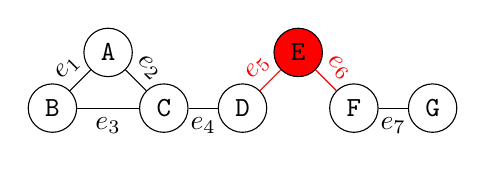
\begin{tikzpicture}[main/.style = {draw, circle}]
        % nodes
        \node[main] (1) {{\tt B}}; 
        \node[main] (2) [above right of=1] {{\tt A}};
        \node[main] (3) [below right of=2] {{\tt C}};
        \node[main] (4) [right of=3] {{\tt D}};
        \node[main, fill=red] (5) [above right of=4] {{\tt E}};
        \node[main] (6) [below right of=5] {{\tt F}};
        \node[main] (7) [right of=6] {{\tt G}};
        % edges
        \draw (1) -- node[midway, above, sloped]{$e_1$} (2);
        \draw (2) -- node[midway, above, sloped]{$e_2$} (3);
        \draw (1) -- node[midway, below, sloped]{$e_3$} (3);
        \draw (3) -- node[midway, below, sloped]{$e_4$}(4);
        \draw[red] (5) -- node[midway, above, sloped]{$e_6$}(6);
        \draw[red] (4) --  node[midway, above, sloped]{$e_5$}(5);
        \draw (6) -- node[midway, below, sloped]{$e_7$}(7);
    \end{tikzpicture} 
    }
\end{center}
\caption{Toy graph example $\mathcal{G}$ with seven nodes ({\tt A} to {\tt G}) and seven edges. Consider a neighboring graph $\mathcal{G}'$ with the differing node {\tt E} (red) and its two edges. }
\label{fig:examplegraph}
\end{figure}

\begin{example}
Let us consider a graph $\mathcal{G}$ with 7 vertices {\tt A} to {\tt G} and 7 edges $e_1$ to $e_7$ as shown in Figure~\ref{fig:examplegraph}. We can have a neighboring graph $\mathcal{G}'$ by considering the vertex {\tt E} as the differing vertex and two of its edges $e_5$ and $e_6$ as the differing edges. This example shows that according to the vanilla 2-approximate algorithm, the output for the graphs $\mathcal{G}$ and $\mathcal{G}'$ may vary drastically. For $\mathcal{G}$, if $e_2$ is selected followed by $e_7$, then the vertex cover size is 4. However, for graph $\mathcal{G}'$, if $e_1$ or $e_4$ is selected first and subsequently after the other one $e_6$ is selected, then the output is 6. Moreover, this difference may get significantly large if the above graph is stacked multiple times and the corresponding vertex that creates this difference is chosen every time. 
\label{example:naive_vertexcover}
\end{example}




\begin{algorithm}[t]
\caption{DP approximation of minimum vertex cover size for $\repair$}
\label{algo:dp_vertexcover}
    \KwData{Graph $\mathcal{G} (V,E)$, stable global ordering $\Lambda$, privacy parameter $\epsilon$}
    \KwResult{DP minimum vertex cover size for $\repair$}
    Initialize vertex cover set $C = \emptyset$ and size $c = 0$ \\
    Initialize edge list $E_0 = E$ \\
    \For{$i \in \{1 \dots |\Lambda|\}$}{
        pop edge $e_i = \{u, v\}$ in order from $\Lambda$\\
        add $u$ and $v$ to $C$ and $c = c + 2$\\
        $E_{i+1}$ = remove all edges incident to $u$ or $v$ from $E_i$\\    
    }
    {\bf Return} $c$\ + Lap($\epsilon$/2)
\end{algorithm}

% We note that the analysis of the algorithm gets complicated because of the random order of the selection of edges. 
% Therefore, inspired by Day et al.~\cite{day2016publishing}, we make a minor change in the algorithm by traversing the edges in a particular order. We use a similar stable ordering $\Lambda$ defined in Section~\ref{sec:prelim-dp}. The updated algorithm is shown in Algorithm~\ref{algo:dp_vertexcover}. We start by initializing an empty vertex cover set $C$ and its size $c$. We then start an iteration over all edges in the same ordering as the stable ordering $\Lambda$. For each edge $e_i = {u,v} \in E$ that is part of the graph, we add both $u$ and $v$ to $C$ and correspondingly increment the size $c$. We also remove all other edges including $e_i$ that are connected to $u$ or $v$ from $E$ and continue the iteration. The sensitivity of this algorithm is given by \cref{prop:vertexcover_sens}. 
To solve the sensitivity issue, we make a minor change in the algorithm by traversing the edges in a particular order (drawing on~\cite{day2016publishing}). We use a similar stable ordering $\Lambda$ defined in \Cref{sec:prelim-dp}. The new algorithm is shown in Algorithm~\ref{algo:dp_vertexcover}. We initialize an empty vertex cover set $C$, its size $c$, and an edge list (lines 1--2). We then start an iteration over all edges in the same ordering as the stable ordering $\Lambda$ (line 3). For each edge $e_i = \{u,v\} \in E$ that is part of the graph, we add both $u$ and $v$ to $C$ and correspondingly increment the size $c$ (lines 4--5). We remove all other edges, including $e_i$, connected to $u$ or $v$ from $E$ and continue the iteration (line 5). Finally, we return the noisy size of the vertex cover (line 6). The sensitivity of this algorithm is given by \cref{prop:vertexcover_sens}. 




\begin{proposition}\label{prop:vertexcover_sens}
Algorithm~\ref{algo:dp_vertexcover} obtains a vertex cover, and its size has a sensitivity of 2.
    % For any two neighboring graphs $\mathcal{G} \neighbor \mathcal{G}^\prime$ that differ by one node, we have
    % \begin{equation*}
    %     \|c - c' \| \leq 2 
    % \end{equation*},
    % where $c$ and $c'$ are the vertex cover sizes of $\mathcal{G}$ and $\mathcal{G}'$ obtained from Algorithm~\ref{algo:dp_vertexcover} respectively.
\end{proposition}



\ifpaper
\begin{proof} (sketch)
Consider two graphs that differ by one node $v^*$ and the edges connected to it. The stable ordering of edges $\Lambda$ in algorithm~\ref{algo:dp_vertexcover} restricts the order in which the edges occur in both graphs. As the algorithm removes all edges of a particular node once observed, we can delineate 3 cases depending on which of the two graphs has the differing node. This allows us to show proof by induction. The detailed proof is in the full version~\cite{full_paper}.
\end{proof}
%Due to space constraints, we defer this proof to the full paper \ag{Add citation when available}. 

\else
The proof can be found in ~\cref{app:vertext_cover_sensitivity}.
\eat{
\proof
Let's assume without loss of generality that
$\mathcal{G}^{\prime}=\left(V^{\prime}, E^{\prime}\right)$ has an additional node $v^{+}$compared to $\mathcal{G}=$ $(V, E)$, i.e., $V^{\prime}=V \cup\left\{v^{+}\right\}, E^{\prime}=E \cup E^{+}$, and $E^{+}$ is the set of all edges incident to $v^{+}$ in $\mathcal{G}^{\prime}$. We prove the theorem using a mathematical induction on $i$ that iterates over all edges of the global stable ordering $\Lambda$.

\underline{Base}: At step 0, the value of $c$ and $c'$ are both 0.

\underline{Hypothesis}: As the algorithm progresses at each step $i$ when the edge $e_i$ is chosen, either the edges of graph $\mathcal{G}'$ which is denoted by $E'_i$ has an extra vertex or the edge of graph $\mathcal{G}$ has an extra vertex. Thus, we can have two cases depending on some node $v^*$ and its edges $\{v^*\}$. Note that at the beginning of the algorithm, $v^*$ is the differing node $v^+$ and $\mathcal{G}'$ has the extra edges of $v^*/v^+$, but $v^*$ may change as the algorithm progresses. The cases are as illustrated below:
\begin{itemize}
    \item Case 1: $E_i$ does not contain any edges incident to $v^*$, $E'_i = E_i + \{ v^* \}$ and the vertex cover sizes at step $i$ could be $c_i = c'_i$ or $c_i = c'_i + 2$.
    \item Case 2: $E'_i$ does not contain any edges incident to $v^*$, $E_i = E'_i + \{ v^* \}$ and the vertex cover sizes at step $i$ could be $c_i = c'_i$ or $c'_i = c_i + 2$.
    \item Case 3: $E_i=E'_i$ and the vertex cover sizes at step $i$ is $c_i = c'_i$. This case occurs only when the additional node $v^+$ has no edges. 
\end{itemize}


\begin{figure*}
    \begin{subfigure}[b]{\textwidth}
    \centering
    \includegraphics[width=0.19\textwidth]{images/true_vs_private/truevsprivate_Stock_positive_degree_nodes_samegraph_10000_rnoise_eps_1.0.jpg}
    \hfill
    \includegraphics[width=0.19\textwidth]{images/true_vs_private/truevsprivate_Tax_positive_degree_nodes_samegraph_10000_rnoise_eps_1.0.jpg}
    \hfill
    \includegraphics[width=0.19\textwidth]{images/true_vs_private/truevsprivate_Hospital_positive_degree_nodes_samegraph_10000_rnoise_eps_1.0.jpg}
    \hfill
    \includegraphics[width=0.19\textwidth]{images/true_vs_private/truevsprivate_Flight_positive_degree_nodes_samegraph_10000_rnoise_eps_1.0.jpg}
    \hfill
    \includegraphics[width=0.19\textwidth]{images/true_vs_private/truevsprivate_Adult_positive_degree_nodes_samegraph_10000_rnoise_eps_1.0.jpg}
    \includegraphics[width=0.2\textwidth]{images/legend_2.png}
    \caption{$\problematic$ (Positive degree nodes)}
    \label{fig:tp_rnoise_pdedges}
    \end{subfigure}
    \begin{subfigure}[b]{\textwidth}
    \centering
    \includegraphics[width=0.19\textwidth]{images/true_vs_private/truevsprivate_Stock_no_of_edges_samegraph_10000_rnoise_eps_1.0_r2t.jpg}
    \hfill
    \includegraphics[width=0.19\textwidth]{images/true_vs_private/truevsprivate_Tax_no_of_edges_samegraph_10000_rnoise_eps_1.0_r2t.jpg}
    \hfill
    \includegraphics[width=0.19\textwidth]{images/true_vs_private/truevsprivate_Hospital_no_of_edges_samegraph_10000_rnoise_eps_1.0_r2t.jpg}
    \hfill
    \includegraphics[width=0.19\textwidth]{images/true_vs_private/truevsprivate_Flight_no_of_edges_samegraph_10000_rnoise_eps_1.0_r2t.jpg}
    \hfill
    \includegraphics[width=0.19\textwidth]{images/true_vs_private/truevsprivate_Adult_no_of_edges_samegraph_10000_rnoise_eps_1.0_r2t.jpg}
    \includegraphics[width=0.3\textwidth]{images/legend2_r2t.png}
    \caption{$\mininconsistency$ (Number of edges)}
    \label{fig:tp_rnoise_nedges}
    \end{subfigure}
      \begin{subfigure}[b]{\textwidth}
         \centering
         \includegraphics[width=0.19\textwidth]{images/true_vs_private/truevsprivate_Stock_vertex_cover_samegraph_10000_rnoise_eps_1.0.jpg}
         \hfill
         \includegraphics[width=0.19\textwidth]{images/true_vs_private/truevsprivate_Tax_vertex_cover_samegraph_10000_rnoise_eps_1.0.jpg}
         \hfill
         \includegraphics[width=0.19\textwidth]{images/true_vs_private/truevsprivate_Hospital_vertex_cover_samegraph_10000_rnoise_eps_1.0.jpg}
         \hfill
         \includegraphics[width=0.19\textwidth]{images/true_vs_private/truevsprivate_Flight_vertex_cover_samegraph_10000_rnoise_eps_1.0.jpg}
         \hfill
         \includegraphics[width=0.19\textwidth]{images/true_vs_private/truevsprivate_Adult_vertex_cover_samegraph_10000_rnoise_eps_1.0.jpg}
         \includegraphics[width=0.2\textwidth]{images/legend_2.png}
         \caption{$\repair$ (Size of vertex cover)}
         \label{fig:tp_rnoise_vcover}
     \end{subfigure}
     \caption{True vs Private estimates for all dataset with RNoise $\alpha = 0.01$ at $\epsilon=1$. The $\problematic$ measure (figure a) and $\mininconsistency$ measure (figure b) are computed using our graph projection approach, and $\repair$ measure using our private vertex cover size approach. }
     \label{fig:tp_RNoise}
\end{figure*}



\underline{Induction}: At step $i+1$, lets assume an edge $e_{i+1} = \{u, v\}$ is chosen. Depending on the $i^{th}$ step, we can have 2 cases as stated in the hypothesis.

\begin{itemize}
    \item Case 1 (When $E'_i$ has the extra edges of $v^*$): We can have the following subcases at step $i+1$ depending on $e_{i+1}$.
        \begin{enumerate}[label=\alph*),ref=\alph*]
            \item If the edge is part of $E'_{i}$ but not of $E_i$ ($e_{i+1} \in E'_{i} \setminus E_{i}$): Then $e_{i+1} = \{u, v\}$ should not exist in $E_i$ (according to the hypothesis at the $i$ step) and one of $u$ or $v$ must be $v^*$. Let's assume without loss of generality that $v$ is $v^*$. The algorithm will add $(u, v)$ to $C'$ and update $c'_{i+1} = c_i + 2$. Hence, we have either $c'_{i+1} = c_{i+1}$ or $c'_{i+1} = c + 2$.

            In addition, all edges of $u$ and $v/v^*$ will be removed from $E'_{i+1}$. Thus, we have $E_{i+1} = E'_{i+1} + \{u\}$, where $\{u\}$ represent edges of $u$. Now $u$ becomes the new $v^*$ and moves to Case 2 for the $i+1$ step.  
            
            \item If the edge is part of both $E'_i$ and $E_i$($e_{i+1} \in E'_i$ and $e_{i+1} \in E_i$): In this case $(u,v)$ will be added to both $C$ and $C'$ and the vertex sizes with be updated as $c_{i+1} = c_i + 2$ and $c'_{i+1} = c' + 2$. 

            Also, the edges adjacent to $u$ and $v$ will be removed from $E_i$ and $E'_i$. We still have $E'_i = E + {v^*}$ (the extra edges of $v^*$ and remain in case 1 for step i+1. 

            \item If the edge is part of neither $E'_i$ nor $E_i$ (If $e_{i+1} \in E'_i$ and $e_{i+1} \in E_i$): the algorithm makes no change. The previous state keep constant: $E'_{i+1} = E'_i, E_{i+1} = E_i$ and $c'_{i+1} = c'_i, c_{i+1} = c_i$. The extra edges of $v^*$ are still in $E'_{i+1}$.
        \end{enumerate}
        
    \item Case 2 (When $E_i$ has the extra edges of $v^*$) : This case is symmetrical to Case 1. There will be three subcases similar to Case 1 -- a) in which after the update, the state of the algorithm switches to Case 1, b) in which the state remains in Case 2, and c) where no update takes place.  

    \item Case 3 (When $E_i = E'_i$): In this case, the algorithm progresses similarly for both the graphs, and remains in case 3 with equal vertex covers, $c_{i+1} = c'_{i+1}$.
\end{itemize}

Our induction proves that our hypothesis is true. The algorithm starts with Case 1, either in the same case or oscillates between Case 1 and Case 2. Hence, as per our hypothesis statement, the difference between the vertex cover sizes is upper-bounded by 2.
\qed
}
\fi



\begin{example}
    Let us consider our running example in Figure~\ref{fig:examplegraph} as input to Algorithm~\ref{algo:dp_vertexcover} and use it to understand the proof. We have two graphs -- $\mathcal{G}$ which has $6$ vertices $V = [{\tt A, B, C, D, F, G}]$ and edges $E = [e_1, e_2, e_3, e_4, e_7]$ and $\mathcal{G}'$ has $7$ vertices $V' = [{\tt A, B, C, D, E, F, G}]$ and edges $E' = [e_1, e_2, \dots, e_7]$. The total possible number of edges is $\binom{7}{2} = 21$, and we can have a global stable ordering of the edges $\Lambda$ depending on the lexicographical ordering of the vertices as $e_1, e_2, e_3, \dots, e_{21}$. When the algorithm starts, both vertex cover sizes are initialized to $c=0, c'=0$, and the algorithm's state is in Case 1 with $v^* = {\tt E}$. We delineate the next steps of the algorithm below:
    \begin{itemize*}
        \item Iteration 1 (Subcase 1b) : $e_1 ({\tt A,B})$ is chosen. {\tt A} and {\tt B} are both in $E_0$ and $E'_0$. Hence $c = 2, c'= 2$.
        \item Iteration 2, 3 (Subcase 1c) : $e_2 ({\tt A,C})$ and $e_3 ({\tt B,C})$ are chosen. Both are removed in iteration 1. Hence $c = 2, c'= 2$.
        \item Iteration 4 (Subcase 1b) : $e_4 ({\tt C, D})$ is chosen. {\tt C} and {\tt D} are both in $E_3$ and $E'_3$. Hence $c = 4, c'= 4$.
        \item Iteration 5 (Subcase 1c) : $e_5 ({\tt D,E})$ is chosen, removed from $E'_4$ in Iteration 4, and was never present in $E$. Hence $c = 4, c'= 4$.
        \item Iteration 6 (Subcase 1a) : $e_6 ({\tt E, F})$ is chosen. It is in $E'_5$ but not in $E_5$. Hence, $c = 4, c'= 6$ and the new $v^* = {\tt E}$.
        \item Iteration 7 (Subcase 2a) : $e_7 ({\tt F,G})$ is chosen. It is in $E_6$ but removed from $E_6$ in Iteration 6. Hence, $c = 6, c'= 6$, and the algorithm is complete.
    \end{itemize*}
\end{example}





\paratitle{Privacy and utility analysis}
We now show the privacy and utility analysis of Algorithm~\ref{algo:dp_vertexcover} using Theorem~\ref{thm:vertex_cover_priv_util_analysis} below.

\begin{theorem}~\label{thm:vertex_cover_priv_util_analysis}
    % Algorithm~\ref{algo:dp_vertexcover} satisfies $\epsilon$-node DP and always outputs the size of a 2-approximate vertex cover of graph $\mathcal{G}$.
    \reva{Algorithm~\ref{algo:dp_vertexcover} satisfies $\epsilon$-node DP and, prior to adding noise in line 7, obtains a 2-approximation vertex cover size.} 
    % of the graph $\mathcal{G}$.}
\end{theorem}

\begin{proof}
The Algorithm~\ref{algo:dp_vertexcover} satisfies $\epsilon$-node DP as we calculate the private vertex cover using the Laplace mechanism with sensitivity $2$ according to Proposition~\ref{prop:vertexcover_sens}. It is also a 2-approximation as the stable ordering $\Lambda$ in Algorithm~\ref{algo:dp_vertexcover} can be perceived as one particular random order of the edges and hence has the same utility as the original 2-approximation algorithm. 
\end{proof}

\section{Experiments}
\label{sec:experiments}
The experiments are designed to address two key research questions.
First, \textbf{RQ1} evaluates whether the average $L_2$-norm of the counterfactual perturbation vectors ($\overline{||\perturb||}$) decreases as the model overfits the data, thereby providing further empirical validation for our hypothesis.
Second, \textbf{RQ2} evaluates the ability of the proposed counterfactual regularized loss, as defined in (\ref{eq:regularized_loss2}), to mitigate overfitting when compared to existing regularization techniques.

% The experiments are designed to address three key research questions. First, \textbf{RQ1} investigates whether the mean perturbation vector norm decreases as the model overfits the data, aiming to further validate our intuition. Second, \textbf{RQ2} explores whether the mean perturbation vector norm can be effectively leveraged as a regularization term during training, offering insights into its potential role in mitigating overfitting. Finally, \textbf{RQ3} examines whether our counterfactual regularizer enables the model to achieve superior performance compared to existing regularization methods, thus highlighting its practical advantage.

\subsection{Experimental Setup}
\textbf{\textit{Datasets, Models, and Tasks.}}
The experiments are conducted on three datasets: \textit{Water Potability}~\cite{kadiwal2020waterpotability}, \textit{Phomene}~\cite{phomene}, and \textit{CIFAR-10}~\cite{krizhevsky2009learning}. For \textit{Water Potability} and \textit{Phomene}, we randomly select $80\%$ of the samples for the training set, and the remaining $20\%$ for the test set, \textit{CIFAR-10} comes already split. Furthermore, we consider the following models: Logistic Regression, Multi-Layer Perceptron (MLP) with 100 and 30 neurons on each hidden layer, and PreactResNet-18~\cite{he2016cvecvv} as a Convolutional Neural Network (CNN) architecture.
We focus on binary classification tasks and leave the extension to multiclass scenarios for future work. However, for datasets that are inherently multiclass, we transform the problem into a binary classification task by selecting two classes, aligning with our assumption.

\smallskip
\noindent\textbf{\textit{Evaluation Measures.}} To characterize the degree of overfitting, we use the test loss, as it serves as a reliable indicator of the model's generalization capability to unseen data. Additionally, we evaluate the predictive performance of each model using the test accuracy.

\smallskip
\noindent\textbf{\textit{Baselines.}} We compare CF-Reg with the following regularization techniques: L1 (``Lasso''), L2 (``Ridge''), and Dropout.

\smallskip
\noindent\textbf{\textit{Configurations.}}
For each model, we adopt specific configurations as follows.
\begin{itemize}
\item \textit{Logistic Regression:} To induce overfitting in the model, we artificially increase the dimensionality of the data beyond the number of training samples by applying a polynomial feature expansion. This approach ensures that the model has enough capacity to overfit the training data, allowing us to analyze the impact of our counterfactual regularizer. The degree of the polynomial is chosen as the smallest degree that makes the number of features greater than the number of data.
\item \textit{Neural Networks (MLP and CNN):} To take advantage of the closed-form solution for computing the optimal perturbation vector as defined in (\ref{eq:opt-delta}), we use a local linear approximation of the neural network models. Hence, given an instance $\inst_i$, we consider the (optimal) counterfactual not with respect to $\model$ but with respect to:
\begin{equation}
\label{eq:taylor}
    \model^{lin}(\inst) = \model(\inst_i) + \nabla_{\inst}\model(\inst_i)(\inst - \inst_i),
\end{equation}
where $\model^{lin}$ represents the first-order Taylor approximation of $\model$ at $\inst_i$.
Note that this step is unnecessary for Logistic Regression, as it is inherently a linear model.
\end{itemize}

\smallskip
\noindent \textbf{\textit{Implementation Details.}} We run all experiments on a machine equipped with an AMD Ryzen 9 7900 12-Core Processor and an NVIDIA GeForce RTX 4090 GPU. Our implementation is based on the PyTorch Lightning framework. We use stochastic gradient descent as the optimizer with a learning rate of $\eta = 0.001$ and no weight decay. We use a batch size of $128$. The training and test steps are conducted for $6000$ epochs on the \textit{Water Potability} and \textit{Phoneme} datasets, while for the \textit{CIFAR-10} dataset, they are performed for $200$ epochs.
Finally, the contribution $w_i^{\varepsilon}$ of each training point $\inst_i$ is uniformly set as $w_i^{\varepsilon} = 1~\forall i\in \{1,\ldots,m\}$.

The source code implementation for our experiments is available at the following GitHub repository: \url{https://anonymous.4open.science/r/COCE-80B4/README.md} 

\subsection{RQ1: Counterfactual Perturbation vs. Overfitting}
To address \textbf{RQ1}, we analyze the relationship between the test loss and the average $L_2$-norm of the counterfactual perturbation vectors ($\overline{||\perturb||}$) over training epochs.

In particular, Figure~\ref{fig:delta_loss_epochs} depicts the evolution of $\overline{||\perturb||}$ alongside the test loss for an MLP trained \textit{without} regularization on the \textit{Water Potability} dataset. 
\begin{figure}[ht]
    \centering
    \includegraphics[width=0.85\linewidth]{img/delta_loss_epochs.png}
    \caption{The average counterfactual perturbation vector $\overline{||\perturb||}$ (left $y$-axis) and the cross-entropy test loss (right $y$-axis) over training epochs ($x$-axis) for an MLP trained on the \textit{Water Potability} dataset \textit{without} regularization.}
    \label{fig:delta_loss_epochs}
\end{figure}

The plot shows a clear trend as the model starts to overfit the data (evidenced by an increase in test loss). 
Notably, $\overline{||\perturb||}$ begins to decrease, which aligns with the hypothesis that the average distance to the optimal counterfactual example gets smaller as the model's decision boundary becomes increasingly adherent to the training data.

It is worth noting that this trend is heavily influenced by the choice of the counterfactual generator model. In particular, the relationship between $\overline{||\perturb||}$ and the degree of overfitting may become even more pronounced when leveraging more accurate counterfactual generators. However, these models often come at the cost of higher computational complexity, and their exploration is left to future work.

Nonetheless, we expect that $\overline{||\perturb||}$ will eventually stabilize at a plateau, as the average $L_2$-norm of the optimal counterfactual perturbations cannot vanish to zero.

% Additionally, the choice of employing the score-based counterfactual explanation framework to generate counterfactuals was driven to promote computational efficiency.

% Future enhancements to the framework may involve adopting models capable of generating more precise counterfactuals. While such approaches may yield to performance improvements, they are likely to come at the cost of increased computational complexity.


\subsection{RQ2: Counterfactual Regularization Performance}
To answer \textbf{RQ2}, we evaluate the effectiveness of the proposed counterfactual regularization (CF-Reg) by comparing its performance against existing baselines: unregularized training loss (No-Reg), L1 regularization (L1-Reg), L2 regularization (L2-Reg), and Dropout.
Specifically, for each model and dataset combination, Table~\ref{tab:regularization_comparison} presents the mean value and standard deviation of test accuracy achieved by each method across 5 random initialization. 

The table illustrates that our regularization technique consistently delivers better results than existing methods across all evaluated scenarios, except for one case -- i.e., Logistic Regression on the \textit{Phomene} dataset. 
However, this setting exhibits an unusual pattern, as the highest model accuracy is achieved without any regularization. Even in this case, CF-Reg still surpasses other regularization baselines.

From the results above, we derive the following key insights. First, CF-Reg proves to be effective across various model types, ranging from simple linear models (Logistic Regression) to deep architectures like MLPs and CNNs, and across diverse datasets, including both tabular and image data. 
Second, CF-Reg's strong performance on the \textit{Water} dataset with Logistic Regression suggests that its benefits may be more pronounced when applied to simpler models. However, the unexpected outcome on the \textit{Phoneme} dataset calls for further investigation into this phenomenon.


\begin{table*}[h!]
    \centering
    \caption{Mean value and standard deviation of test accuracy across 5 random initializations for different model, dataset, and regularization method. The best results are highlighted in \textbf{bold}.}
    \label{tab:regularization_comparison}
    \begin{tabular}{|c|c|c|c|c|c|c|}
        \hline
        \textbf{Model} & \textbf{Dataset} & \textbf{No-Reg} & \textbf{L1-Reg} & \textbf{L2-Reg} & \textbf{Dropout} & \textbf{CF-Reg (ours)} \\ \hline
        Logistic Regression   & \textit{Water}   & $0.6595 \pm 0.0038$   & $0.6729 \pm 0.0056$   & $0.6756 \pm 0.0046$  & N/A    & $\mathbf{0.6918 \pm 0.0036}$                     \\ \hline
        MLP   & \textit{Water}   & $0.6756 \pm 0.0042$   & $0.6790 \pm 0.0058$   & $0.6790 \pm 0.0023$  & $0.6750 \pm 0.0036$    & $\mathbf{0.6802 \pm 0.0046}$                    \\ \hline
%        MLP   & \textit{Adult}   & $0.8404 \pm 0.0010$   & $\mathbf{0.8495 \pm 0.0007}$   & $0.8489 \pm 0.0014$  & $\mathbf{0.8495 \pm 0.0016}$     & $0.8449 \pm 0.0019$                    \\ \hline
        Logistic Regression   & \textit{Phomene}   & $\mathbf{0.8148 \pm 0.0020}$   & $0.8041 \pm 0.0028$   & $0.7835 \pm 0.0176$  & N/A    & $0.8098 \pm 0.0055$                     \\ \hline
        MLP   & \textit{Phomene}   & $0.8677 \pm 0.0033$   & $0.8374 \pm 0.0080$   & $0.8673 \pm 0.0045$  & $0.8672 \pm 0.0042$     & $\mathbf{0.8718 \pm 0.0040}$                    \\ \hline
        CNN   & \textit{CIFAR-10} & $0.6670 \pm 0.0233$   & $0.6229 \pm 0.0850$   & $0.7348 \pm 0.0365$   & N/A    & $\mathbf{0.7427 \pm 0.0571}$                     \\ \hline
    \end{tabular}
\end{table*}

\begin{table*}[htb!]
    \centering
    \caption{Hyperparameter configurations utilized for the generation of Table \ref{tab:regularization_comparison}. For our regularization the hyperparameters are reported as $\mathbf{\alpha/\beta}$.}
    \label{tab:performance_parameters}
    \begin{tabular}{|c|c|c|c|c|c|c|}
        \hline
        \textbf{Model} & \textbf{Dataset} & \textbf{No-Reg} & \textbf{L1-Reg} & \textbf{L2-Reg} & \textbf{Dropout} & \textbf{CF-Reg (ours)} \\ \hline
        Logistic Regression   & \textit{Water}   & N/A   & $0.0093$   & $0.6927$  & N/A    & $0.3791/1.0355$                     \\ \hline
        MLP   & \textit{Water}   & N/A   & $0.0007$   & $0.0022$  & $0.0002$    & $0.2567/1.9775$                    \\ \hline
        Logistic Regression   &
        \textit{Phomene}   & N/A   & $0.0097$   & $0.7979$  & N/A    & $0.0571/1.8516$                     \\ \hline
        MLP   & \textit{Phomene}   & N/A   & $0.0007$   & $4.24\cdot10^{-5}$  & $0.0015$    & $0.0516/2.2700$                    \\ \hline
       % MLP   & \textit{Adult}   & N/A   & $0.0018$   & $0.0018$  & $0.0601$     & $0.0764/2.2068$                    \\ \hline
        CNN   & \textit{CIFAR-10} & N/A   & $0.0050$   & $0.0864$ & N/A    & $0.3018/
        2.1502$                     \\ \hline
    \end{tabular}
\end{table*}

\begin{table*}[htb!]
    \centering
    \caption{Mean value and standard deviation of training time across 5 different runs. The reported time (in seconds) corresponds to the generation of each entry in Table \ref{tab:regularization_comparison}. Times are }
    \label{tab:times}
    \begin{tabular}{|c|c|c|c|c|c|c|}
        \hline
        \textbf{Model} & \textbf{Dataset} & \textbf{No-Reg} & \textbf{L1-Reg} & \textbf{L2-Reg} & \textbf{Dropout} & \textbf{CF-Reg (ours)} \\ \hline
        Logistic Regression   & \textit{Water}   & $222.98 \pm 1.07$   & $239.94 \pm 2.59$   & $241.60 \pm 1.88$  & N/A    & $251.50 \pm 1.93$                     \\ \hline
        MLP   & \textit{Water}   & $225.71 \pm 3.85$   & $250.13 \pm 4.44$   & $255.78 \pm 2.38$  & $237.83 \pm 3.45$    & $266.48 \pm 3.46$                    \\ \hline
        Logistic Regression   & \textit{Phomene}   & $266.39 \pm 0.82$ & $367.52 \pm 6.85$   & $361.69 \pm 4.04$  & N/A   & $310.48 \pm 0.76$                    \\ \hline
        MLP   &
        \textit{Phomene} & $335.62 \pm 1.77$   & $390.86 \pm 2.11$   & $393.96 \pm 1.95$ & $363.51 \pm 5.07$    & $403.14 \pm 1.92$                     \\ \hline
       % MLP   & \textit{Adult}   & N/A   & $0.0018$   & $0.0018$  & $0.0601$     & $0.0764/2.2068$                    \\ \hline
        CNN   & \textit{CIFAR-10} & $370.09 \pm 0.18$   & $395.71 \pm 0.55$   & $401.38 \pm 0.16$ & N/A    & $1287.8 \pm 0.26$                     \\ \hline
    \end{tabular}
\end{table*}

\subsection{Feasibility of our Method}
A crucial requirement for any regularization technique is that it should impose minimal impact on the overall training process.
In this respect, CF-Reg introduces an overhead that depends on the time required to find the optimal counterfactual example for each training instance. 
As such, the more sophisticated the counterfactual generator model probed during training the higher would be the time required. However, a more advanced counterfactual generator might provide a more effective regularization. We discuss this trade-off in more details in Section~\ref{sec:discussion}.

Table~\ref{tab:times} presents the average training time ($\pm$ standard deviation) for each model and dataset combination listed in Table~\ref{tab:regularization_comparison}.
We can observe that the higher accuracy achieved by CF-Reg using the score-based counterfactual generator comes with only minimal overhead. However, when applied to deep neural networks with many hidden layers, such as \textit{PreactResNet-18}, the forward derivative computation required for the linearization of the network introduces a more noticeable computational cost, explaining the longer training times in the table.

\subsection{Hyperparameter Sensitivity Analysis}
The proposed counterfactual regularization technique relies on two key hyperparameters: $\alpha$ and $\beta$. The former is intrinsic to the loss formulation defined in (\ref{eq:cf-train}), while the latter is closely tied to the choice of the score-based counterfactual explanation method used.

Figure~\ref{fig:test_alpha_beta} illustrates how the test accuracy of an MLP trained on the \textit{Water Potability} dataset changes for different combinations of $\alpha$ and $\beta$.

\begin{figure}[ht]
    \centering
    \includegraphics[width=0.85\linewidth]{img/test_acc_alpha_beta.png}
    \caption{The test accuracy of an MLP trained on the \textit{Water Potability} dataset, evaluated while varying the weight of our counterfactual regularizer ($\alpha$) for different values of $\beta$.}
    \label{fig:test_alpha_beta}
\end{figure}

We observe that, for a fixed $\beta$, increasing the weight of our counterfactual regularizer ($\alpha$) can slightly improve test accuracy until a sudden drop is noticed for $\alpha > 0.1$.
This behavior was expected, as the impact of our penalty, like any regularization term, can be disruptive if not properly controlled.

Moreover, this finding further demonstrates that our regularization method, CF-Reg, is inherently data-driven. Therefore, it requires specific fine-tuning based on the combination of the model and dataset at hand.
\putsec{related}{Related Work}

\noindent \textbf{Efficient Radiance Field Rendering.}
%
The introduction of Neural Radiance Fields (NeRF)~\cite{mil:sri20} has
generated significant interest in efficient 3D scene representation and
rendering for radiance fields.
%
Over the past years, there has been a large amount of research aimed at
accelerating NeRFs through algorithmic or software
optimizations~\cite{mul:eva22,fri:yu22,che:fun23,sun:sun22}, and the
development of hardware
accelerators~\cite{lee:cho23,li:li23,son:wen23,mub:kan23,fen:liu24}.
%
The state-of-the-art method, 3D Gaussian splatting~\cite{ker:kop23}, has
further fueled interest in accelerating radiance field
rendering~\cite{rad:ste24,lee:lee24,nie:stu24,lee:rho24,ham:mel24} as it
employs rasterization primitives that can be rendered much faster than NeRFs.
%
However, previous research focused on software graphics rendering on
programmable cores or building dedicated hardware accelerators. In contrast,
\name{} investigates the potential of efficient radiance field rendering while
utilizing fixed-function units in graphics hardware.
%
To our knowledge, this is the first work that assesses the performance
implications of rendering Gaussian-based radiance fields on the hardware
graphics pipeline with software and hardware optimizations.

%%%%%%%%%%%%%%%%%%%%%%%%%%%%%%%%%%%%%%%%%%%%%%%%%%%%%%%%%%%%%%%%%%%%%%%%%%
\myparagraph{Enhancing Graphics Rendering Hardware.}
%
The performance advantage of executing graphics rendering on either
programmable shader cores or fixed-function units varies depending on the
rendering methods and hardware designs.
%
Previous studies have explored the performance implication of graphics hardware
design by developing simulation infrastructures for graphics
workloads~\cite{bar:gon06,gub:aam19,tin:sax23,arn:par13}.
%
Additionally, several studies have aimed to improve the performance of
special-purpose hardware such as ray tracing units in graphics
hardware~\cite{cho:now23,liu:cha21} and proposed hardware accelerators for
graphics applications~\cite{lu:hua17,ram:gri09}.
%
In contrast to these works, which primarily evaluate traditional graphics
workloads, our work focuses on improving the performance of volume rendering
workloads, such as Gaussian splatting, which require blending a huge number of
fragments per pixel.

%%%%%%%%%%%%%%%%%%%%%%%%%%%%%%%%%%%%%%%%%%%%%%%%%%%%%%%%%%%%%%%%%%%%%%%%%%
%
In the context of multi-sample anti-aliasing, prior work proposed reducing the
amount of redundant shading by merging fragments from adjacent triangles in a
mesh at the quad granularity~\cite{fat:bou10}.
%
While both our work and quad-fragment merging (QFM)~\cite{fat:bou10} aim to
reduce operations by merging quads, our proposed technique differs from QFM in
many aspects.
%
Our method aims to blend \emph{overlapping primitives} along the depth
direction and applies to quads from any primitive. In contrast, QFM merges quad
fragments from small (e.g., pixel-sized) triangles that \emph{share} an edge
(i.e., \emph{connected}, \emph{non-overlapping} triangles).
%
As such, QFM is not applicable to the scenes consisting of a number of
unconnected transparent triangles, such as those in 3D Gaussian splatting.
%
In addition, our method computes the \emph{exact} color for each pixel by
offloading blending operations from ROPs to shader units, whereas QFM
\emph{approximates} pixel colors by using the color from one triangle when
multiple triangles are merged into a single quad.


\vspace{-0.2cm}
\section{Impact: Why Free Scientific Knowledge?}
\vspace{-0.1cm}

Historically, making knowledge widely available has driven transformative progress. Gutenberg’s printing press broke medieval monopolies on information, increasing literacy and contributing to the Renaissance and Scientific Revolution. In today's world, open source projects such as GNU/Linux and Wikipedia show that freely accessible and modifiable knowledge fosters innovation while ensuring creators are credited through copyleft licenses. These examples highlight a key idea: \textit{access to essential knowledge supports overall advancement.} 

This aligns with the arguments made by Prabhakaran et al. \cite{humanrightsbasedapproachresponsible}, who specifically highlight the \textbf{ human right to participate in scientific advancement} as enshrined in the Universal Declaration of Human Rights. They emphasize that this right underscores the importance of \textit{ equal access to the benefits of scientific progress for all}, a principle directly supported by our proposal for Knowledge Units. The UN Special Rapporteur on Cultural Rights further reinforces this, advocating for the expansion of copyright exceptions to broaden access to scientific knowledge as a crucial component of the right to science and culture \cite{scienceright}. 

However, current intellectual property regimes often create ``patently unfair" barriers to this knowledge, preventing innovation and access, especially in areas critical to human rights, as Hale compellingly argues \cite{patentlyunfair}. Finding a solution requires carefully balancing the imperative of open access with the legitimate rights of authors. As Austin and Ginsburg remind us, authors' rights are also human rights, necessitating robust protection \cite{authorhumanrights}. Shareable knowledge entities like Knowledge Units offer a potential mechanism to achieve this delicate balance in the scientific domain, enabling wider dissemination of research findings while respecting authors' fundamental rights.

\vspace{-0.2cm}
\subsection{Impact Across Sectors}

\textbf{Researchers:} Collaboration across different fields becomes easier when knowledge is shared openly. For instance, combining machine learning with biology or applying quantum principles to cryptography can lead to important breakthroughs. Removing copyright restrictions allows researchers to freely use data and methods, speeding up discoveries while respecting original contributions.

\textbf{Practitioners:} Professionals, especially in healthcare, benefit from immediate access to the latest research. Quick access to newer insights on the effectiveness of drugs, and alternative treatments speeds up adoption and awareness, potentially saving lives. Additionally, open knowledge helps developing countries gain access to health innovations.

\textbf{Education:} Education becomes more accessible when teachers use the latest research to create up-to-date curricula without prohibitive costs. Students can access high-quality research materials and use LM assistance to better understand complex topics, enhancing their learning experience and making high-quality education more accessible.

\textbf{Public Trust:} When information is transparent and accessible, the public can better understand and trust decision-making processes. Open access to government policies and industry practices allows people to review and verify information, helping to reduce misinformation. This transparency encourages critical thinking and builds trust in scientific and governmental institutions.

Overall, making scientific knowledge accessible supports global fairness. By viewing knowledge as a common resource rather than a product to be sold, we can speed up innovation, encourage critical thinking, and empower communities to address important challenges.

\vspace{-0.2cm}
\section{Open Problems}
\vspace{-0.1cm}

Moving forward, we identify key research directions to further exploit the potential of converting original texts into shareable knowledge entities such as demonstrated by the conversion into Knowledge Units in this work:


\textbf{1. Enhancing Factual Accuracy and Reliability:}  Refining KUs through cross-referencing with source texts and incorporating community-driven correction mechanisms, similar to Wikipedia, can minimize hallucinations and ensure the long-term accuracy of knowledge-based datasets at scale.

\textbf{2. Developing Applications for Education and Research:}  Using KU-based conversion for datasets to be employed in practical tools, such as search interfaces and learning platforms, can ensure rapid dissemination of any new knowledge into shareable downstream resources, significantly improving the accessibility, spread, and impact of KUs.

\textbf{3. Establishing Standards for Knowledge Interoperability and Reuse:}  Future research should focus on defining standardized formats for entities like KU and knowledge graph layouts \citep{lenat1990cyc}. These standards are essential to unlock seamless interoperability, facilitate reuse across diverse platforms, and foster a vibrant ecosystem of open scientific knowledge. 

\textbf{4. Interconnecting Shareable Knowledge for Scientific Workflow Assistance and Automation:} There might be further potential in constructing a semantic web that interconnects publicly shared knowledge, together with mechanisms that continually update and validate all shareable knowledge units. This can be starting point for a platform that uses all collected knowledge to assist scientific workflows, for instance by feeding such a semantic web into recently developed reasoning models equipped with retrieval augmented generation. Such assistance could assemble knowledge across multiple scientific papers, guiding scientists more efficiently through vast research landscapes. Given further progress in model capabilities, validation, self-repair and evolving new knowledge from already existing vast collection in the semantic web can lead to automation of scientific discovery, assuming that knowledge data in the semantic web can be freely shared.

We open-source our code and encourage collaboration to improve extraction pipelines, enhance Knowledge Unit capabilities, and expand coverage to additional fields.

\vspace{-0.2cm}
\section{Conclusion}
\vspace{-0.1cm}

In this paper, we highlight the potential of systematically separating factual scientific knowledge from protected artistic or stylistic expression. By representing scientific insights as structured facts and relationships, prototypes like Knowledge Units (KUs) offer a pathway to broaden access to scientific knowledge without infringing copyright, aligning with legal principles like German \S 24(1) UrhG and U.S. fair use standards. Extensive testing across a range of domains and models shows evidence that Knowledge Units (KUs) can feasibly retain core information. These findings offer a promising way forward for openly disseminating scientific information while respecting copyright constraints.

\section*{Author Contributions}

Christoph conceived the project and led organization. Christoph and Gollam led all the experiments. Nick and Huu led the legal aspects. Tawsif led the data collection. Ameya and Andreas led the manuscript writing. Ludwig, Sören, Robert, Jenia and Matthias provided feedback. advice and scientific supervision throughout the project. 

\section*{Acknowledgements}

The authors would like to thank (in alphabetical order): Sebastian Dziadzio, Kristof Meding, Tea Mustać, Shantanu Prabhat for insightful feedback and suggestions. Special thanks to Andrej Radonjic for help in scaling up data collection. GR and SA acknowledge financial support by the German Research Foundation (DFG) for the NFDI4DataScience Initiative (project number 460234259). AP and MB acknowledge financial support by the Federal Ministry of Education and Research (BMBF), FKZ: 011524085B and Open Philanthropy Foundation funded by the Good Ventures Foundation. AH acknowledges financial support by the Federal Ministry of Education and Research (BMBF), FKZ: 01IS24079A and the Carl Zeiss Foundation through the project "Certification and Foundations of Safe ML Systems" as well as the support from the International Max Planck Research School for Intelligent Systems (IMPRS-IS). JJ acknowledges funding by the Federal Ministry of Education and Research of Germany (BMBF) under grant no. 01IS22094B (WestAI - AI Service Center West), under grant no. 01IS24085C (OPENHAFM) and under the grant DE002571 (MINERVA), as well as co-funding by EU from EuroHPC Joint Undertaking programm under grant no. 101182737 (MINERVA) and from Digital Europe Programme under grant no. 101195233 (openEuroLLM) 

%%
%% The acknowledgments section is defined using the "acks" environment
%% (and NOT an unnumbered section). This ensures the proper
%% identification of the section in the article metadata, and the
%% consistent spelling of the heading.
\begin{acks}
Shubhankar Mohapatra was supported by an Ontario graduate, vector graduate research, and David R. Cheriton scholarships. The work of Xi He was supported by NSERC through a Discovery Grant, an alliance grant, and the Canada CIFAR AI Chairs program. The work of Amir Gilad was funded by the Israel Science Foundation (ISF) under grant 1702/24, the Scharf-Ullman Endowment, and the Alon Scholarship. 
\end{acks}

%%
%% The next two lines define the bibliography style to be used, and
%% the bibliography file.

\newpage
\balance
\bibliographystyle{ACM-Reference-Format}
\bibliography{bibtex}


%%
%% If your work has an appendix, this is the place to put it.
\ifpaper

% \subsection{Lloyd-Max Algorithm}
\label{subsec:Lloyd-Max}
For a given quantization bitwidth $B$ and an operand $\bm{X}$, the Lloyd-Max algorithm finds $2^B$ quantization levels $\{\hat{x}_i\}_{i=1}^{2^B}$ such that quantizing $\bm{X}$ by rounding each scalar in $\bm{X}$ to the nearest quantization level minimizes the quantization MSE. 

The algorithm starts with an initial guess of quantization levels and then iteratively computes quantization thresholds $\{\tau_i\}_{i=1}^{2^B-1}$ and updates quantization levels $\{\hat{x}_i\}_{i=1}^{2^B}$. Specifically, at iteration $n$, thresholds are set to the midpoints of the previous iteration's levels:
\begin{align*}
    \tau_i^{(n)}=\frac{\hat{x}_i^{(n-1)}+\hat{x}_{i+1}^{(n-1)}}2 \text{ for } i=1\ldots 2^B-1
\end{align*}
Subsequently, the quantization levels are re-computed as conditional means of the data regions defined by the new thresholds:
\begin{align*}
    \hat{x}_i^{(n)}=\mathbb{E}\left[ \bm{X} \big| \bm{X}\in [\tau_{i-1}^{(n)},\tau_i^{(n)}] \right] \text{ for } i=1\ldots 2^B
\end{align*}
where to satisfy boundary conditions we have $\tau_0=-\infty$ and $\tau_{2^B}=\infty$. The algorithm iterates the above steps until convergence.

Figure \ref{fig:lm_quant} compares the quantization levels of a $7$-bit floating point (E3M3) quantizer (left) to a $7$-bit Lloyd-Max quantizer (right) when quantizing a layer of weights from the GPT3-126M model at a per-tensor granularity. As shown, the Lloyd-Max quantizer achieves substantially lower quantization MSE. Further, Table \ref{tab:FP7_vs_LM7} shows the superior perplexity achieved by Lloyd-Max quantizers for bitwidths of $7$, $6$ and $5$. The difference between the quantizers is clear at 5 bits, where per-tensor FP quantization incurs a drastic and unacceptable increase in perplexity, while Lloyd-Max quantization incurs a much smaller increase. Nevertheless, we note that even the optimal Lloyd-Max quantizer incurs a notable ($\sim 1.5$) increase in perplexity due to the coarse granularity of quantization. 

\begin{figure}[h]
  \centering
  \includegraphics[width=0.7\linewidth]{sections/figures/LM7_FP7.pdf}
  \caption{\small Quantization levels and the corresponding quantization MSE of Floating Point (left) vs Lloyd-Max (right) Quantizers for a layer of weights in the GPT3-126M model.}
  \label{fig:lm_quant}
\end{figure}

\begin{table}[h]\scriptsize
\begin{center}
\caption{\label{tab:FP7_vs_LM7} \small Comparing perplexity (lower is better) achieved by floating point quantizers and Lloyd-Max quantizers on a GPT3-126M model for the Wikitext-103 dataset.}
\begin{tabular}{c|cc|c}
\hline
 \multirow{2}{*}{\textbf{Bitwidth}} & \multicolumn{2}{|c|}{\textbf{Floating-Point Quantizer}} & \textbf{Lloyd-Max Quantizer} \\
 & Best Format & Wikitext-103 Perplexity & Wikitext-103 Perplexity \\
\hline
7 & E3M3 & 18.32 & 18.27 \\
6 & E3M2 & 19.07 & 18.51 \\
5 & E4M0 & 43.89 & 19.71 \\
\hline
\end{tabular}
\end{center}
\end{table}

\subsection{Proof of Local Optimality of LO-BCQ}
\label{subsec:lobcq_opt_proof}
For a given block $\bm{b}_j$, the quantization MSE during LO-BCQ can be empirically evaluated as $\frac{1}{L_b}\lVert \bm{b}_j- \bm{\hat{b}}_j\rVert^2_2$ where $\bm{\hat{b}}_j$ is computed from equation (\ref{eq:clustered_quantization_definition}) as $C_{f(\bm{b}_j)}(\bm{b}_j)$. Further, for a given block cluster $\mathcal{B}_i$, we compute the quantization MSE as $\frac{1}{|\mathcal{B}_{i}|}\sum_{\bm{b} \in \mathcal{B}_{i}} \frac{1}{L_b}\lVert \bm{b}- C_i^{(n)}(\bm{b})\rVert^2_2$. Therefore, at the end of iteration $n$, we evaluate the overall quantization MSE $J^{(n)}$ for a given operand $\bm{X}$ composed of $N_c$ block clusters as:
\begin{align*}
    \label{eq:mse_iter_n}
    J^{(n)} = \frac{1}{N_c} \sum_{i=1}^{N_c} \frac{1}{|\mathcal{B}_{i}^{(n)}|}\sum_{\bm{v} \in \mathcal{B}_{i}^{(n)}} \frac{1}{L_b}\lVert \bm{b}- B_i^{(n)}(\bm{b})\rVert^2_2
\end{align*}

At the end of iteration $n$, the codebooks are updated from $\mathcal{C}^{(n-1)}$ to $\mathcal{C}^{(n)}$. However, the mapping of a given vector $\bm{b}_j$ to quantizers $\mathcal{C}^{(n)}$ remains as  $f^{(n)}(\bm{b}_j)$. At the next iteration, during the vector clustering step, $f^{(n+1)}(\bm{b}_j)$ finds new mapping of $\bm{b}_j$ to updated codebooks $\mathcal{C}^{(n)}$ such that the quantization MSE over the candidate codebooks is minimized. Therefore, we obtain the following result for $\bm{b}_j$:
\begin{align*}
\frac{1}{L_b}\lVert \bm{b}_j - C_{f^{(n+1)}(\bm{b}_j)}^{(n)}(\bm{b}_j)\rVert^2_2 \le \frac{1}{L_b}\lVert \bm{b}_j - C_{f^{(n)}(\bm{b}_j)}^{(n)}(\bm{b}_j)\rVert^2_2
\end{align*}

That is, quantizing $\bm{b}_j$ at the end of the block clustering step of iteration $n+1$ results in lower quantization MSE compared to quantizing at the end of iteration $n$. Since this is true for all $\bm{b} \in \bm{X}$, we assert the following:
\begin{equation}
\begin{split}
\label{eq:mse_ineq_1}
    \tilde{J}^{(n+1)} &= \frac{1}{N_c} \sum_{i=1}^{N_c} \frac{1}{|\mathcal{B}_{i}^{(n+1)}|}\sum_{\bm{b} \in \mathcal{B}_{i}^{(n+1)}} \frac{1}{L_b}\lVert \bm{b} - C_i^{(n)}(b)\rVert^2_2 \le J^{(n)}
\end{split}
\end{equation}
where $\tilde{J}^{(n+1)}$ is the the quantization MSE after the vector clustering step at iteration $n+1$.

Next, during the codebook update step (\ref{eq:quantizers_update}) at iteration $n+1$, the per-cluster codebooks $\mathcal{C}^{(n)}$ are updated to $\mathcal{C}^{(n+1)}$ by invoking the Lloyd-Max algorithm \citep{Lloyd}. We know that for any given value distribution, the Lloyd-Max algorithm minimizes the quantization MSE. Therefore, for a given vector cluster $\mathcal{B}_i$ we obtain the following result:

\begin{equation}
    \frac{1}{|\mathcal{B}_{i}^{(n+1)}|}\sum_{\bm{b} \in \mathcal{B}_{i}^{(n+1)}} \frac{1}{L_b}\lVert \bm{b}- C_i^{(n+1)}(\bm{b})\rVert^2_2 \le \frac{1}{|\mathcal{B}_{i}^{(n+1)}|}\sum_{\bm{b} \in \mathcal{B}_{i}^{(n+1)}} \frac{1}{L_b}\lVert \bm{b}- C_i^{(n)}(\bm{b})\rVert^2_2
\end{equation}

The above equation states that quantizing the given block cluster $\mathcal{B}_i$ after updating the associated codebook from $C_i^{(n)}$ to $C_i^{(n+1)}$ results in lower quantization MSE. Since this is true for all the block clusters, we derive the following result: 
\begin{equation}
\begin{split}
\label{eq:mse_ineq_2}
     J^{(n+1)} &= \frac{1}{N_c} \sum_{i=1}^{N_c} \frac{1}{|\mathcal{B}_{i}^{(n+1)}|}\sum_{\bm{b} \in \mathcal{B}_{i}^{(n+1)}} \frac{1}{L_b}\lVert \bm{b}- C_i^{(n+1)}(\bm{b})\rVert^2_2  \le \tilde{J}^{(n+1)}   
\end{split}
\end{equation}

Following (\ref{eq:mse_ineq_1}) and (\ref{eq:mse_ineq_2}), we find that the quantization MSE is non-increasing for each iteration, that is, $J^{(1)} \ge J^{(2)} \ge J^{(3)} \ge \ldots \ge J^{(M)}$ where $M$ is the maximum number of iterations. 
%Therefore, we can say that if the algorithm converges, then it must be that it has converged to a local minimum. 
\hfill $\blacksquare$


\begin{figure}
    \begin{center}
    \includegraphics[width=0.5\textwidth]{sections//figures/mse_vs_iter.pdf}
    \end{center}
    \caption{\small NMSE vs iterations during LO-BCQ compared to other block quantization proposals}
    \label{fig:nmse_vs_iter}
\end{figure}

Figure \ref{fig:nmse_vs_iter} shows the empirical convergence of LO-BCQ across several block lengths and number of codebooks. Also, the MSE achieved by LO-BCQ is compared to baselines such as MXFP and VSQ. As shown, LO-BCQ converges to a lower MSE than the baselines. Further, we achieve better convergence for larger number of codebooks ($N_c$) and for a smaller block length ($L_b$), both of which increase the bitwidth of BCQ (see Eq \ref{eq:bitwidth_bcq}).


\subsection{Additional Accuracy Results}
%Table \ref{tab:lobcq_config} lists the various LOBCQ configurations and their corresponding bitwidths.
\begin{table}
\setlength{\tabcolsep}{4.75pt}
\begin{center}
\caption{\label{tab:lobcq_config} Various LO-BCQ configurations and their bitwidths.}
\begin{tabular}{|c||c|c|c|c||c|c||c|} 
\hline
 & \multicolumn{4}{|c||}{$L_b=8$} & \multicolumn{2}{|c||}{$L_b=4$} & $L_b=2$ \\
 \hline
 \backslashbox{$L_A$\kern-1em}{\kern-1em$N_c$} & 2 & 4 & 8 & 16 & 2 & 4 & 2 \\
 \hline
 64 & 4.25 & 4.375 & 4.5 & 4.625 & 4.375 & 4.625 & 4.625\\
 \hline
 32 & 4.375 & 4.5 & 4.625& 4.75 & 4.5 & 4.75 & 4.75 \\
 \hline
 16 & 4.625 & 4.75& 4.875 & 5 & 4.75 & 5 & 5 \\
 \hline
\end{tabular}
\end{center}
\end{table}

%\subsection{Perplexity achieved by various LO-BCQ configurations on Wikitext-103 dataset}

\begin{table} \centering
\begin{tabular}{|c||c|c|c|c||c|c||c|} 
\hline
 $L_b \rightarrow$& \multicolumn{4}{c||}{8} & \multicolumn{2}{c||}{4} & 2\\
 \hline
 \backslashbox{$L_A$\kern-1em}{\kern-1em$N_c$} & 2 & 4 & 8 & 16 & 2 & 4 & 2  \\
 %$N_c \rightarrow$ & 2 & 4 & 8 & 16 & 2 & 4 & 2 \\
 \hline
 \hline
 \multicolumn{8}{c}{GPT3-1.3B (FP32 PPL = 9.98)} \\ 
 \hline
 \hline
 64 & 10.40 & 10.23 & 10.17 & 10.15 &  10.28 & 10.18 & 10.19 \\
 \hline
 32 & 10.25 & 10.20 & 10.15 & 10.12 &  10.23 & 10.17 & 10.17 \\
 \hline
 16 & 10.22 & 10.16 & 10.10 & 10.09 &  10.21 & 10.14 & 10.16 \\
 \hline
  \hline
 \multicolumn{8}{c}{GPT3-8B (FP32 PPL = 7.38)} \\ 
 \hline
 \hline
 64 & 7.61 & 7.52 & 7.48 &  7.47 &  7.55 &  7.49 & 7.50 \\
 \hline
 32 & 7.52 & 7.50 & 7.46 &  7.45 &  7.52 &  7.48 & 7.48  \\
 \hline
 16 & 7.51 & 7.48 & 7.44 &  7.44 &  7.51 &  7.49 & 7.47  \\
 \hline
\end{tabular}
\caption{\label{tab:ppl_gpt3_abalation} Wikitext-103 perplexity across GPT3-1.3B and 8B models.}
\end{table}

\begin{table} \centering
\begin{tabular}{|c||c|c|c|c||} 
\hline
 $L_b \rightarrow$& \multicolumn{4}{c||}{8}\\
 \hline
 \backslashbox{$L_A$\kern-1em}{\kern-1em$N_c$} & 2 & 4 & 8 & 16 \\
 %$N_c \rightarrow$ & 2 & 4 & 8 & 16 & 2 & 4 & 2 \\
 \hline
 \hline
 \multicolumn{5}{|c|}{Llama2-7B (FP32 PPL = 5.06)} \\ 
 \hline
 \hline
 64 & 5.31 & 5.26 & 5.19 & 5.18  \\
 \hline
 32 & 5.23 & 5.25 & 5.18 & 5.15  \\
 \hline
 16 & 5.23 & 5.19 & 5.16 & 5.14  \\
 \hline
 \multicolumn{5}{|c|}{Nemotron4-15B (FP32 PPL = 5.87)} \\ 
 \hline
 \hline
 64  & 6.3 & 6.20 & 6.13 & 6.08  \\
 \hline
 32  & 6.24 & 6.12 & 6.07 & 6.03  \\
 \hline
 16  & 6.12 & 6.14 & 6.04 & 6.02  \\
 \hline
 \multicolumn{5}{|c|}{Nemotron4-340B (FP32 PPL = 3.48)} \\ 
 \hline
 \hline
 64 & 3.67 & 3.62 & 3.60 & 3.59 \\
 \hline
 32 & 3.63 & 3.61 & 3.59 & 3.56 \\
 \hline
 16 & 3.61 & 3.58 & 3.57 & 3.55 \\
 \hline
\end{tabular}
\caption{\label{tab:ppl_llama7B_nemo15B} Wikitext-103 perplexity compared to FP32 baseline in Llama2-7B and Nemotron4-15B, 340B models}
\end{table}

%\subsection{Perplexity achieved by various LO-BCQ configurations on MMLU dataset}


\begin{table} \centering
\begin{tabular}{|c||c|c|c|c||c|c|c|c|} 
\hline
 $L_b \rightarrow$& \multicolumn{4}{c||}{8} & \multicolumn{4}{c||}{8}\\
 \hline
 \backslashbox{$L_A$\kern-1em}{\kern-1em$N_c$} & 2 & 4 & 8 & 16 & 2 & 4 & 8 & 16  \\
 %$N_c \rightarrow$ & 2 & 4 & 8 & 16 & 2 & 4 & 2 \\
 \hline
 \hline
 \multicolumn{5}{|c|}{Llama2-7B (FP32 Accuracy = 45.8\%)} & \multicolumn{4}{|c|}{Llama2-70B (FP32 Accuracy = 69.12\%)} \\ 
 \hline
 \hline
 64 & 43.9 & 43.4 & 43.9 & 44.9 & 68.07 & 68.27 & 68.17 & 68.75 \\
 \hline
 32 & 44.5 & 43.8 & 44.9 & 44.5 & 68.37 & 68.51 & 68.35 & 68.27  \\
 \hline
 16 & 43.9 & 42.7 & 44.9 & 45 & 68.12 & 68.77 & 68.31 & 68.59  \\
 \hline
 \hline
 \multicolumn{5}{|c|}{GPT3-22B (FP32 Accuracy = 38.75\%)} & \multicolumn{4}{|c|}{Nemotron4-15B (FP32 Accuracy = 64.3\%)} \\ 
 \hline
 \hline
 64 & 36.71 & 38.85 & 38.13 & 38.92 & 63.17 & 62.36 & 63.72 & 64.09 \\
 \hline
 32 & 37.95 & 38.69 & 39.45 & 38.34 & 64.05 & 62.30 & 63.8 & 64.33  \\
 \hline
 16 & 38.88 & 38.80 & 38.31 & 38.92 & 63.22 & 63.51 & 63.93 & 64.43  \\
 \hline
\end{tabular}
\caption{\label{tab:mmlu_abalation} Accuracy on MMLU dataset across GPT3-22B, Llama2-7B, 70B and Nemotron4-15B models.}
\end{table}


%\subsection{Perplexity achieved by various LO-BCQ configurations on LM evaluation harness}

\begin{table} \centering
\begin{tabular}{|c||c|c|c|c||c|c|c|c|} 
\hline
 $L_b \rightarrow$& \multicolumn{4}{c||}{8} & \multicolumn{4}{c||}{8}\\
 \hline
 \backslashbox{$L_A$\kern-1em}{\kern-1em$N_c$} & 2 & 4 & 8 & 16 & 2 & 4 & 8 & 16  \\
 %$N_c \rightarrow$ & 2 & 4 & 8 & 16 & 2 & 4 & 2 \\
 \hline
 \hline
 \multicolumn{5}{|c|}{Race (FP32 Accuracy = 37.51\%)} & \multicolumn{4}{|c|}{Boolq (FP32 Accuracy = 64.62\%)} \\ 
 \hline
 \hline
 64 & 36.94 & 37.13 & 36.27 & 37.13 & 63.73 & 62.26 & 63.49 & 63.36 \\
 \hline
 32 & 37.03 & 36.36 & 36.08 & 37.03 & 62.54 & 63.51 & 63.49 & 63.55  \\
 \hline
 16 & 37.03 & 37.03 & 36.46 & 37.03 & 61.1 & 63.79 & 63.58 & 63.33  \\
 \hline
 \hline
 \multicolumn{5}{|c|}{Winogrande (FP32 Accuracy = 58.01\%)} & \multicolumn{4}{|c|}{Piqa (FP32 Accuracy = 74.21\%)} \\ 
 \hline
 \hline
 64 & 58.17 & 57.22 & 57.85 & 58.33 & 73.01 & 73.07 & 73.07 & 72.80 \\
 \hline
 32 & 59.12 & 58.09 & 57.85 & 58.41 & 73.01 & 73.94 & 72.74 & 73.18  \\
 \hline
 16 & 57.93 & 58.88 & 57.93 & 58.56 & 73.94 & 72.80 & 73.01 & 73.94  \\
 \hline
\end{tabular}
\caption{\label{tab:mmlu_abalation} Accuracy on LM evaluation harness tasks on GPT3-1.3B model.}
\end{table}

\begin{table} \centering
\begin{tabular}{|c||c|c|c|c||c|c|c|c|} 
\hline
 $L_b \rightarrow$& \multicolumn{4}{c||}{8} & \multicolumn{4}{c||}{8}\\
 \hline
 \backslashbox{$L_A$\kern-1em}{\kern-1em$N_c$} & 2 & 4 & 8 & 16 & 2 & 4 & 8 & 16  \\
 %$N_c \rightarrow$ & 2 & 4 & 8 & 16 & 2 & 4 & 2 \\
 \hline
 \hline
 \multicolumn{5}{|c|}{Race (FP32 Accuracy = 41.34\%)} & \multicolumn{4}{|c|}{Boolq (FP32 Accuracy = 68.32\%)} \\ 
 \hline
 \hline
 64 & 40.48 & 40.10 & 39.43 & 39.90 & 69.20 & 68.41 & 69.45 & 68.56 \\
 \hline
 32 & 39.52 & 39.52 & 40.77 & 39.62 & 68.32 & 67.43 & 68.17 & 69.30  \\
 \hline
 16 & 39.81 & 39.71 & 39.90 & 40.38 & 68.10 & 66.33 & 69.51 & 69.42  \\
 \hline
 \hline
 \multicolumn{5}{|c|}{Winogrande (FP32 Accuracy = 67.88\%)} & \multicolumn{4}{|c|}{Piqa (FP32 Accuracy = 78.78\%)} \\ 
 \hline
 \hline
 64 & 66.85 & 66.61 & 67.72 & 67.88 & 77.31 & 77.42 & 77.75 & 77.64 \\
 \hline
 32 & 67.25 & 67.72 & 67.72 & 67.00 & 77.31 & 77.04 & 77.80 & 77.37  \\
 \hline
 16 & 68.11 & 68.90 & 67.88 & 67.48 & 77.37 & 78.13 & 78.13 & 77.69  \\
 \hline
\end{tabular}
\caption{\label{tab:mmlu_abalation} Accuracy on LM evaluation harness tasks on GPT3-8B model.}
\end{table}

\begin{table} \centering
\begin{tabular}{|c||c|c|c|c||c|c|c|c|} 
\hline
 $L_b \rightarrow$& \multicolumn{4}{c||}{8} & \multicolumn{4}{c||}{8}\\
 \hline
 \backslashbox{$L_A$\kern-1em}{\kern-1em$N_c$} & 2 & 4 & 8 & 16 & 2 & 4 & 8 & 16  \\
 %$N_c \rightarrow$ & 2 & 4 & 8 & 16 & 2 & 4 & 2 \\
 \hline
 \hline
 \multicolumn{5}{|c|}{Race (FP32 Accuracy = 40.67\%)} & \multicolumn{4}{|c|}{Boolq (FP32 Accuracy = 76.54\%)} \\ 
 \hline
 \hline
 64 & 40.48 & 40.10 & 39.43 & 39.90 & 75.41 & 75.11 & 77.09 & 75.66 \\
 \hline
 32 & 39.52 & 39.52 & 40.77 & 39.62 & 76.02 & 76.02 & 75.96 & 75.35  \\
 \hline
 16 & 39.81 & 39.71 & 39.90 & 40.38 & 75.05 & 73.82 & 75.72 & 76.09  \\
 \hline
 \hline
 \multicolumn{5}{|c|}{Winogrande (FP32 Accuracy = 70.64\%)} & \multicolumn{4}{|c|}{Piqa (FP32 Accuracy = 79.16\%)} \\ 
 \hline
 \hline
 64 & 69.14 & 70.17 & 70.17 & 70.56 & 78.24 & 79.00 & 78.62 & 78.73 \\
 \hline
 32 & 70.96 & 69.69 & 71.27 & 69.30 & 78.56 & 79.49 & 79.16 & 78.89  \\
 \hline
 16 & 71.03 & 69.53 & 69.69 & 70.40 & 78.13 & 79.16 & 79.00 & 79.00  \\
 \hline
\end{tabular}
\caption{\label{tab:mmlu_abalation} Accuracy on LM evaluation harness tasks on GPT3-22B model.}
\end{table}

\begin{table} \centering
\begin{tabular}{|c||c|c|c|c||c|c|c|c|} 
\hline
 $L_b \rightarrow$& \multicolumn{4}{c||}{8} & \multicolumn{4}{c||}{8}\\
 \hline
 \backslashbox{$L_A$\kern-1em}{\kern-1em$N_c$} & 2 & 4 & 8 & 16 & 2 & 4 & 8 & 16  \\
 %$N_c \rightarrow$ & 2 & 4 & 8 & 16 & 2 & 4 & 2 \\
 \hline
 \hline
 \multicolumn{5}{|c|}{Race (FP32 Accuracy = 44.4\%)} & \multicolumn{4}{|c|}{Boolq (FP32 Accuracy = 79.29\%)} \\ 
 \hline
 \hline
 64 & 42.49 & 42.51 & 42.58 & 43.45 & 77.58 & 77.37 & 77.43 & 78.1 \\
 \hline
 32 & 43.35 & 42.49 & 43.64 & 43.73 & 77.86 & 75.32 & 77.28 & 77.86  \\
 \hline
 16 & 44.21 & 44.21 & 43.64 & 42.97 & 78.65 & 77 & 76.94 & 77.98  \\
 \hline
 \hline
 \multicolumn{5}{|c|}{Winogrande (FP32 Accuracy = 69.38\%)} & \multicolumn{4}{|c|}{Piqa (FP32 Accuracy = 78.07\%)} \\ 
 \hline
 \hline
 64 & 68.9 & 68.43 & 69.77 & 68.19 & 77.09 & 76.82 & 77.09 & 77.86 \\
 \hline
 32 & 69.38 & 68.51 & 68.82 & 68.90 & 78.07 & 76.71 & 78.07 & 77.86  \\
 \hline
 16 & 69.53 & 67.09 & 69.38 & 68.90 & 77.37 & 77.8 & 77.91 & 77.69  \\
 \hline
\end{tabular}
\caption{\label{tab:mmlu_abalation} Accuracy on LM evaluation harness tasks on Llama2-7B model.}
\end{table}

\begin{table} \centering
\begin{tabular}{|c||c|c|c|c||c|c|c|c|} 
\hline
 $L_b \rightarrow$& \multicolumn{4}{c||}{8} & \multicolumn{4}{c||}{8}\\
 \hline
 \backslashbox{$L_A$\kern-1em}{\kern-1em$N_c$} & 2 & 4 & 8 & 16 & 2 & 4 & 8 & 16  \\
 %$N_c \rightarrow$ & 2 & 4 & 8 & 16 & 2 & 4 & 2 \\
 \hline
 \hline
 \multicolumn{5}{|c|}{Race (FP32 Accuracy = 48.8\%)} & \multicolumn{4}{|c|}{Boolq (FP32 Accuracy = 85.23\%)} \\ 
 \hline
 \hline
 64 & 49.00 & 49.00 & 49.28 & 48.71 & 82.82 & 84.28 & 84.03 & 84.25 \\
 \hline
 32 & 49.57 & 48.52 & 48.33 & 49.28 & 83.85 & 84.46 & 84.31 & 84.93  \\
 \hline
 16 & 49.85 & 49.09 & 49.28 & 48.99 & 85.11 & 84.46 & 84.61 & 83.94  \\
 \hline
 \hline
 \multicolumn{5}{|c|}{Winogrande (FP32 Accuracy = 79.95\%)} & \multicolumn{4}{|c|}{Piqa (FP32 Accuracy = 81.56\%)} \\ 
 \hline
 \hline
 64 & 78.77 & 78.45 & 78.37 & 79.16 & 81.45 & 80.69 & 81.45 & 81.5 \\
 \hline
 32 & 78.45 & 79.01 & 78.69 & 80.66 & 81.56 & 80.58 & 81.18 & 81.34  \\
 \hline
 16 & 79.95 & 79.56 & 79.79 & 79.72 & 81.28 & 81.66 & 81.28 & 80.96  \\
 \hline
\end{tabular}
\caption{\label{tab:mmlu_abalation} Accuracy on LM evaluation harness tasks on Llama2-70B model.}
\end{table}

%\section{MSE Studies}
%\textcolor{red}{TODO}


\subsection{Number Formats and Quantization Method}
\label{subsec:numFormats_quantMethod}
\subsubsection{Integer Format}
An $n$-bit signed integer (INT) is typically represented with a 2s-complement format \citep{yao2022zeroquant,xiao2023smoothquant,dai2021vsq}, where the most significant bit denotes the sign.

\subsubsection{Floating Point Format}
An $n$-bit signed floating point (FP) number $x$ comprises of a 1-bit sign ($x_{\mathrm{sign}}$), $B_m$-bit mantissa ($x_{\mathrm{mant}}$) and $B_e$-bit exponent ($x_{\mathrm{exp}}$) such that $B_m+B_e=n-1$. The associated constant exponent bias ($E_{\mathrm{bias}}$) is computed as $(2^{{B_e}-1}-1)$. We denote this format as $E_{B_e}M_{B_m}$.  

\subsubsection{Quantization Scheme}
\label{subsec:quant_method}
A quantization scheme dictates how a given unquantized tensor is converted to its quantized representation. We consider FP formats for the purpose of illustration. Given an unquantized tensor $\bm{X}$ and an FP format $E_{B_e}M_{B_m}$, we first, we compute the quantization scale factor $s_X$ that maps the maximum absolute value of $\bm{X}$ to the maximum quantization level of the $E_{B_e}M_{B_m}$ format as follows:
\begin{align}
\label{eq:sf}
    s_X = \frac{\mathrm{max}(|\bm{X}|)}{\mathrm{max}(E_{B_e}M_{B_m})}
\end{align}
In the above equation, $|\cdot|$ denotes the absolute value function.

Next, we scale $\bm{X}$ by $s_X$ and quantize it to $\hat{\bm{X}}$ by rounding it to the nearest quantization level of $E_{B_e}M_{B_m}$ as:

\begin{align}
\label{eq:tensor_quant}
    \hat{\bm{X}} = \text{round-to-nearest}\left(\frac{\bm{X}}{s_X}, E_{B_e}M_{B_m}\right)
\end{align}

We perform dynamic max-scaled quantization \citep{wu2020integer}, where the scale factor $s$ for activations is dynamically computed during runtime.

\subsection{Vector Scaled Quantization}
\begin{wrapfigure}{r}{0.35\linewidth}
  \centering
  \includegraphics[width=\linewidth]{sections/figures/vsquant.jpg}
  \caption{\small Vectorwise decomposition for per-vector scaled quantization (VSQ \citep{dai2021vsq}).}
  \label{fig:vsquant}
\end{wrapfigure}
During VSQ \citep{dai2021vsq}, the operand tensors are decomposed into 1D vectors in a hardware friendly manner as shown in Figure \ref{fig:vsquant}. Since the decomposed tensors are used as operands in matrix multiplications during inference, it is beneficial to perform this decomposition along the reduction dimension of the multiplication. The vectorwise quantization is performed similar to tensorwise quantization described in Equations \ref{eq:sf} and \ref{eq:tensor_quant}, where a scale factor $s_v$ is required for each vector $\bm{v}$ that maps the maximum absolute value of that vector to the maximum quantization level. While smaller vector lengths can lead to larger accuracy gains, the associated memory and computational overheads due to the per-vector scale factors increases. To alleviate these overheads, VSQ \citep{dai2021vsq} proposed a second level quantization of the per-vector scale factors to unsigned integers, while MX \citep{rouhani2023shared} quantizes them to integer powers of 2 (denoted as $2^{INT}$).

\subsubsection{MX Format}
The MX format proposed in \citep{rouhani2023microscaling} introduces the concept of sub-block shifting. For every two scalar elements of $b$-bits each, there is a shared exponent bit. The value of this exponent bit is determined through an empirical analysis that targets minimizing quantization MSE. We note that the FP format $E_{1}M_{b}$ is strictly better than MX from an accuracy perspective since it allocates a dedicated exponent bit to each scalar as opposed to sharing it across two scalars. Therefore, we conservatively bound the accuracy of a $b+2$-bit signed MX format with that of a $E_{1}M_{b}$ format in our comparisons. For instance, we use E1M2 format as a proxy for MX4.

\begin{figure}
    \centering
    \includegraphics[width=1\linewidth]{sections//figures/BlockFormats.pdf}
    \caption{\small Comparing LO-BCQ to MX format.}
    \label{fig:block_formats}
\end{figure}

Figure \ref{fig:block_formats} compares our $4$-bit LO-BCQ block format to MX \citep{rouhani2023microscaling}. As shown, both LO-BCQ and MX decompose a given operand tensor into block arrays and each block array into blocks. Similar to MX, we find that per-block quantization ($L_b < L_A$) leads to better accuracy due to increased flexibility. While MX achieves this through per-block $1$-bit micro-scales, we associate a dedicated codebook to each block through a per-block codebook selector. Further, MX quantizes the per-block array scale-factor to E8M0 format without per-tensor scaling. In contrast during LO-BCQ, we find that per-tensor scaling combined with quantization of per-block array scale-factor to E4M3 format results in superior inference accuracy across models. 
  %%comment it out when for submission 
\else
\newpage 
\subsection{Lloyd-Max Algorithm}
\label{subsec:Lloyd-Max}
For a given quantization bitwidth $B$ and an operand $\bm{X}$, the Lloyd-Max algorithm finds $2^B$ quantization levels $\{\hat{x}_i\}_{i=1}^{2^B}$ such that quantizing $\bm{X}$ by rounding each scalar in $\bm{X}$ to the nearest quantization level minimizes the quantization MSE. 

The algorithm starts with an initial guess of quantization levels and then iteratively computes quantization thresholds $\{\tau_i\}_{i=1}^{2^B-1}$ and updates quantization levels $\{\hat{x}_i\}_{i=1}^{2^B}$. Specifically, at iteration $n$, thresholds are set to the midpoints of the previous iteration's levels:
\begin{align*}
    \tau_i^{(n)}=\frac{\hat{x}_i^{(n-1)}+\hat{x}_{i+1}^{(n-1)}}2 \text{ for } i=1\ldots 2^B-1
\end{align*}
Subsequently, the quantization levels are re-computed as conditional means of the data regions defined by the new thresholds:
\begin{align*}
    \hat{x}_i^{(n)}=\mathbb{E}\left[ \bm{X} \big| \bm{X}\in [\tau_{i-1}^{(n)},\tau_i^{(n)}] \right] \text{ for } i=1\ldots 2^B
\end{align*}
where to satisfy boundary conditions we have $\tau_0=-\infty$ and $\tau_{2^B}=\infty$. The algorithm iterates the above steps until convergence.

Figure \ref{fig:lm_quant} compares the quantization levels of a $7$-bit floating point (E3M3) quantizer (left) to a $7$-bit Lloyd-Max quantizer (right) when quantizing a layer of weights from the GPT3-126M model at a per-tensor granularity. As shown, the Lloyd-Max quantizer achieves substantially lower quantization MSE. Further, Table \ref{tab:FP7_vs_LM7} shows the superior perplexity achieved by Lloyd-Max quantizers for bitwidths of $7$, $6$ and $5$. The difference between the quantizers is clear at 5 bits, where per-tensor FP quantization incurs a drastic and unacceptable increase in perplexity, while Lloyd-Max quantization incurs a much smaller increase. Nevertheless, we note that even the optimal Lloyd-Max quantizer incurs a notable ($\sim 1.5$) increase in perplexity due to the coarse granularity of quantization. 

\begin{figure}[h]
  \centering
  \includegraphics[width=0.7\linewidth]{sections/figures/LM7_FP7.pdf}
  \caption{\small Quantization levels and the corresponding quantization MSE of Floating Point (left) vs Lloyd-Max (right) Quantizers for a layer of weights in the GPT3-126M model.}
  \label{fig:lm_quant}
\end{figure}

\begin{table}[h]\scriptsize
\begin{center}
\caption{\label{tab:FP7_vs_LM7} \small Comparing perplexity (lower is better) achieved by floating point quantizers and Lloyd-Max quantizers on a GPT3-126M model for the Wikitext-103 dataset.}
\begin{tabular}{c|cc|c}
\hline
 \multirow{2}{*}{\textbf{Bitwidth}} & \multicolumn{2}{|c|}{\textbf{Floating-Point Quantizer}} & \textbf{Lloyd-Max Quantizer} \\
 & Best Format & Wikitext-103 Perplexity & Wikitext-103 Perplexity \\
\hline
7 & E3M3 & 18.32 & 18.27 \\
6 & E3M2 & 19.07 & 18.51 \\
5 & E4M0 & 43.89 & 19.71 \\
\hline
\end{tabular}
\end{center}
\end{table}

\subsection{Proof of Local Optimality of LO-BCQ}
\label{subsec:lobcq_opt_proof}
For a given block $\bm{b}_j$, the quantization MSE during LO-BCQ can be empirically evaluated as $\frac{1}{L_b}\lVert \bm{b}_j- \bm{\hat{b}}_j\rVert^2_2$ where $\bm{\hat{b}}_j$ is computed from equation (\ref{eq:clustered_quantization_definition}) as $C_{f(\bm{b}_j)}(\bm{b}_j)$. Further, for a given block cluster $\mathcal{B}_i$, we compute the quantization MSE as $\frac{1}{|\mathcal{B}_{i}|}\sum_{\bm{b} \in \mathcal{B}_{i}} \frac{1}{L_b}\lVert \bm{b}- C_i^{(n)}(\bm{b})\rVert^2_2$. Therefore, at the end of iteration $n$, we evaluate the overall quantization MSE $J^{(n)}$ for a given operand $\bm{X}$ composed of $N_c$ block clusters as:
\begin{align*}
    \label{eq:mse_iter_n}
    J^{(n)} = \frac{1}{N_c} \sum_{i=1}^{N_c} \frac{1}{|\mathcal{B}_{i}^{(n)}|}\sum_{\bm{v} \in \mathcal{B}_{i}^{(n)}} \frac{1}{L_b}\lVert \bm{b}- B_i^{(n)}(\bm{b})\rVert^2_2
\end{align*}

At the end of iteration $n$, the codebooks are updated from $\mathcal{C}^{(n-1)}$ to $\mathcal{C}^{(n)}$. However, the mapping of a given vector $\bm{b}_j$ to quantizers $\mathcal{C}^{(n)}$ remains as  $f^{(n)}(\bm{b}_j)$. At the next iteration, during the vector clustering step, $f^{(n+1)}(\bm{b}_j)$ finds new mapping of $\bm{b}_j$ to updated codebooks $\mathcal{C}^{(n)}$ such that the quantization MSE over the candidate codebooks is minimized. Therefore, we obtain the following result for $\bm{b}_j$:
\begin{align*}
\frac{1}{L_b}\lVert \bm{b}_j - C_{f^{(n+1)}(\bm{b}_j)}^{(n)}(\bm{b}_j)\rVert^2_2 \le \frac{1}{L_b}\lVert \bm{b}_j - C_{f^{(n)}(\bm{b}_j)}^{(n)}(\bm{b}_j)\rVert^2_2
\end{align*}

That is, quantizing $\bm{b}_j$ at the end of the block clustering step of iteration $n+1$ results in lower quantization MSE compared to quantizing at the end of iteration $n$. Since this is true for all $\bm{b} \in \bm{X}$, we assert the following:
\begin{equation}
\begin{split}
\label{eq:mse_ineq_1}
    \tilde{J}^{(n+1)} &= \frac{1}{N_c} \sum_{i=1}^{N_c} \frac{1}{|\mathcal{B}_{i}^{(n+1)}|}\sum_{\bm{b} \in \mathcal{B}_{i}^{(n+1)}} \frac{1}{L_b}\lVert \bm{b} - C_i^{(n)}(b)\rVert^2_2 \le J^{(n)}
\end{split}
\end{equation}
where $\tilde{J}^{(n+1)}$ is the the quantization MSE after the vector clustering step at iteration $n+1$.

Next, during the codebook update step (\ref{eq:quantizers_update}) at iteration $n+1$, the per-cluster codebooks $\mathcal{C}^{(n)}$ are updated to $\mathcal{C}^{(n+1)}$ by invoking the Lloyd-Max algorithm \citep{Lloyd}. We know that for any given value distribution, the Lloyd-Max algorithm minimizes the quantization MSE. Therefore, for a given vector cluster $\mathcal{B}_i$ we obtain the following result:

\begin{equation}
    \frac{1}{|\mathcal{B}_{i}^{(n+1)}|}\sum_{\bm{b} \in \mathcal{B}_{i}^{(n+1)}} \frac{1}{L_b}\lVert \bm{b}- C_i^{(n+1)}(\bm{b})\rVert^2_2 \le \frac{1}{|\mathcal{B}_{i}^{(n+1)}|}\sum_{\bm{b} \in \mathcal{B}_{i}^{(n+1)}} \frac{1}{L_b}\lVert \bm{b}- C_i^{(n)}(\bm{b})\rVert^2_2
\end{equation}

The above equation states that quantizing the given block cluster $\mathcal{B}_i$ after updating the associated codebook from $C_i^{(n)}$ to $C_i^{(n+1)}$ results in lower quantization MSE. Since this is true for all the block clusters, we derive the following result: 
\begin{equation}
\begin{split}
\label{eq:mse_ineq_2}
     J^{(n+1)} &= \frac{1}{N_c} \sum_{i=1}^{N_c} \frac{1}{|\mathcal{B}_{i}^{(n+1)}|}\sum_{\bm{b} \in \mathcal{B}_{i}^{(n+1)}} \frac{1}{L_b}\lVert \bm{b}- C_i^{(n+1)}(\bm{b})\rVert^2_2  \le \tilde{J}^{(n+1)}   
\end{split}
\end{equation}

Following (\ref{eq:mse_ineq_1}) and (\ref{eq:mse_ineq_2}), we find that the quantization MSE is non-increasing for each iteration, that is, $J^{(1)} \ge J^{(2)} \ge J^{(3)} \ge \ldots \ge J^{(M)}$ where $M$ is the maximum number of iterations. 
%Therefore, we can say that if the algorithm converges, then it must be that it has converged to a local minimum. 
\hfill $\blacksquare$


\begin{figure}
    \begin{center}
    \includegraphics[width=0.5\textwidth]{sections//figures/mse_vs_iter.pdf}
    \end{center}
    \caption{\small NMSE vs iterations during LO-BCQ compared to other block quantization proposals}
    \label{fig:nmse_vs_iter}
\end{figure}

Figure \ref{fig:nmse_vs_iter} shows the empirical convergence of LO-BCQ across several block lengths and number of codebooks. Also, the MSE achieved by LO-BCQ is compared to baselines such as MXFP and VSQ. As shown, LO-BCQ converges to a lower MSE than the baselines. Further, we achieve better convergence for larger number of codebooks ($N_c$) and for a smaller block length ($L_b$), both of which increase the bitwidth of BCQ (see Eq \ref{eq:bitwidth_bcq}).


\subsection{Additional Accuracy Results}
%Table \ref{tab:lobcq_config} lists the various LOBCQ configurations and their corresponding bitwidths.
\begin{table}
\setlength{\tabcolsep}{4.75pt}
\begin{center}
\caption{\label{tab:lobcq_config} Various LO-BCQ configurations and their bitwidths.}
\begin{tabular}{|c||c|c|c|c||c|c||c|} 
\hline
 & \multicolumn{4}{|c||}{$L_b=8$} & \multicolumn{2}{|c||}{$L_b=4$} & $L_b=2$ \\
 \hline
 \backslashbox{$L_A$\kern-1em}{\kern-1em$N_c$} & 2 & 4 & 8 & 16 & 2 & 4 & 2 \\
 \hline
 64 & 4.25 & 4.375 & 4.5 & 4.625 & 4.375 & 4.625 & 4.625\\
 \hline
 32 & 4.375 & 4.5 & 4.625& 4.75 & 4.5 & 4.75 & 4.75 \\
 \hline
 16 & 4.625 & 4.75& 4.875 & 5 & 4.75 & 5 & 5 \\
 \hline
\end{tabular}
\end{center}
\end{table}

%\subsection{Perplexity achieved by various LO-BCQ configurations on Wikitext-103 dataset}

\begin{table} \centering
\begin{tabular}{|c||c|c|c|c||c|c||c|} 
\hline
 $L_b \rightarrow$& \multicolumn{4}{c||}{8} & \multicolumn{2}{c||}{4} & 2\\
 \hline
 \backslashbox{$L_A$\kern-1em}{\kern-1em$N_c$} & 2 & 4 & 8 & 16 & 2 & 4 & 2  \\
 %$N_c \rightarrow$ & 2 & 4 & 8 & 16 & 2 & 4 & 2 \\
 \hline
 \hline
 \multicolumn{8}{c}{GPT3-1.3B (FP32 PPL = 9.98)} \\ 
 \hline
 \hline
 64 & 10.40 & 10.23 & 10.17 & 10.15 &  10.28 & 10.18 & 10.19 \\
 \hline
 32 & 10.25 & 10.20 & 10.15 & 10.12 &  10.23 & 10.17 & 10.17 \\
 \hline
 16 & 10.22 & 10.16 & 10.10 & 10.09 &  10.21 & 10.14 & 10.16 \\
 \hline
  \hline
 \multicolumn{8}{c}{GPT3-8B (FP32 PPL = 7.38)} \\ 
 \hline
 \hline
 64 & 7.61 & 7.52 & 7.48 &  7.47 &  7.55 &  7.49 & 7.50 \\
 \hline
 32 & 7.52 & 7.50 & 7.46 &  7.45 &  7.52 &  7.48 & 7.48  \\
 \hline
 16 & 7.51 & 7.48 & 7.44 &  7.44 &  7.51 &  7.49 & 7.47  \\
 \hline
\end{tabular}
\caption{\label{tab:ppl_gpt3_abalation} Wikitext-103 perplexity across GPT3-1.3B and 8B models.}
\end{table}

\begin{table} \centering
\begin{tabular}{|c||c|c|c|c||} 
\hline
 $L_b \rightarrow$& \multicolumn{4}{c||}{8}\\
 \hline
 \backslashbox{$L_A$\kern-1em}{\kern-1em$N_c$} & 2 & 4 & 8 & 16 \\
 %$N_c \rightarrow$ & 2 & 4 & 8 & 16 & 2 & 4 & 2 \\
 \hline
 \hline
 \multicolumn{5}{|c|}{Llama2-7B (FP32 PPL = 5.06)} \\ 
 \hline
 \hline
 64 & 5.31 & 5.26 & 5.19 & 5.18  \\
 \hline
 32 & 5.23 & 5.25 & 5.18 & 5.15  \\
 \hline
 16 & 5.23 & 5.19 & 5.16 & 5.14  \\
 \hline
 \multicolumn{5}{|c|}{Nemotron4-15B (FP32 PPL = 5.87)} \\ 
 \hline
 \hline
 64  & 6.3 & 6.20 & 6.13 & 6.08  \\
 \hline
 32  & 6.24 & 6.12 & 6.07 & 6.03  \\
 \hline
 16  & 6.12 & 6.14 & 6.04 & 6.02  \\
 \hline
 \multicolumn{5}{|c|}{Nemotron4-340B (FP32 PPL = 3.48)} \\ 
 \hline
 \hline
 64 & 3.67 & 3.62 & 3.60 & 3.59 \\
 \hline
 32 & 3.63 & 3.61 & 3.59 & 3.56 \\
 \hline
 16 & 3.61 & 3.58 & 3.57 & 3.55 \\
 \hline
\end{tabular}
\caption{\label{tab:ppl_llama7B_nemo15B} Wikitext-103 perplexity compared to FP32 baseline in Llama2-7B and Nemotron4-15B, 340B models}
\end{table}

%\subsection{Perplexity achieved by various LO-BCQ configurations on MMLU dataset}


\begin{table} \centering
\begin{tabular}{|c||c|c|c|c||c|c|c|c|} 
\hline
 $L_b \rightarrow$& \multicolumn{4}{c||}{8} & \multicolumn{4}{c||}{8}\\
 \hline
 \backslashbox{$L_A$\kern-1em}{\kern-1em$N_c$} & 2 & 4 & 8 & 16 & 2 & 4 & 8 & 16  \\
 %$N_c \rightarrow$ & 2 & 4 & 8 & 16 & 2 & 4 & 2 \\
 \hline
 \hline
 \multicolumn{5}{|c|}{Llama2-7B (FP32 Accuracy = 45.8\%)} & \multicolumn{4}{|c|}{Llama2-70B (FP32 Accuracy = 69.12\%)} \\ 
 \hline
 \hline
 64 & 43.9 & 43.4 & 43.9 & 44.9 & 68.07 & 68.27 & 68.17 & 68.75 \\
 \hline
 32 & 44.5 & 43.8 & 44.9 & 44.5 & 68.37 & 68.51 & 68.35 & 68.27  \\
 \hline
 16 & 43.9 & 42.7 & 44.9 & 45 & 68.12 & 68.77 & 68.31 & 68.59  \\
 \hline
 \hline
 \multicolumn{5}{|c|}{GPT3-22B (FP32 Accuracy = 38.75\%)} & \multicolumn{4}{|c|}{Nemotron4-15B (FP32 Accuracy = 64.3\%)} \\ 
 \hline
 \hline
 64 & 36.71 & 38.85 & 38.13 & 38.92 & 63.17 & 62.36 & 63.72 & 64.09 \\
 \hline
 32 & 37.95 & 38.69 & 39.45 & 38.34 & 64.05 & 62.30 & 63.8 & 64.33  \\
 \hline
 16 & 38.88 & 38.80 & 38.31 & 38.92 & 63.22 & 63.51 & 63.93 & 64.43  \\
 \hline
\end{tabular}
\caption{\label{tab:mmlu_abalation} Accuracy on MMLU dataset across GPT3-22B, Llama2-7B, 70B and Nemotron4-15B models.}
\end{table}


%\subsection{Perplexity achieved by various LO-BCQ configurations on LM evaluation harness}

\begin{table} \centering
\begin{tabular}{|c||c|c|c|c||c|c|c|c|} 
\hline
 $L_b \rightarrow$& \multicolumn{4}{c||}{8} & \multicolumn{4}{c||}{8}\\
 \hline
 \backslashbox{$L_A$\kern-1em}{\kern-1em$N_c$} & 2 & 4 & 8 & 16 & 2 & 4 & 8 & 16  \\
 %$N_c \rightarrow$ & 2 & 4 & 8 & 16 & 2 & 4 & 2 \\
 \hline
 \hline
 \multicolumn{5}{|c|}{Race (FP32 Accuracy = 37.51\%)} & \multicolumn{4}{|c|}{Boolq (FP32 Accuracy = 64.62\%)} \\ 
 \hline
 \hline
 64 & 36.94 & 37.13 & 36.27 & 37.13 & 63.73 & 62.26 & 63.49 & 63.36 \\
 \hline
 32 & 37.03 & 36.36 & 36.08 & 37.03 & 62.54 & 63.51 & 63.49 & 63.55  \\
 \hline
 16 & 37.03 & 37.03 & 36.46 & 37.03 & 61.1 & 63.79 & 63.58 & 63.33  \\
 \hline
 \hline
 \multicolumn{5}{|c|}{Winogrande (FP32 Accuracy = 58.01\%)} & \multicolumn{4}{|c|}{Piqa (FP32 Accuracy = 74.21\%)} \\ 
 \hline
 \hline
 64 & 58.17 & 57.22 & 57.85 & 58.33 & 73.01 & 73.07 & 73.07 & 72.80 \\
 \hline
 32 & 59.12 & 58.09 & 57.85 & 58.41 & 73.01 & 73.94 & 72.74 & 73.18  \\
 \hline
 16 & 57.93 & 58.88 & 57.93 & 58.56 & 73.94 & 72.80 & 73.01 & 73.94  \\
 \hline
\end{tabular}
\caption{\label{tab:mmlu_abalation} Accuracy on LM evaluation harness tasks on GPT3-1.3B model.}
\end{table}

\begin{table} \centering
\begin{tabular}{|c||c|c|c|c||c|c|c|c|} 
\hline
 $L_b \rightarrow$& \multicolumn{4}{c||}{8} & \multicolumn{4}{c||}{8}\\
 \hline
 \backslashbox{$L_A$\kern-1em}{\kern-1em$N_c$} & 2 & 4 & 8 & 16 & 2 & 4 & 8 & 16  \\
 %$N_c \rightarrow$ & 2 & 4 & 8 & 16 & 2 & 4 & 2 \\
 \hline
 \hline
 \multicolumn{5}{|c|}{Race (FP32 Accuracy = 41.34\%)} & \multicolumn{4}{|c|}{Boolq (FP32 Accuracy = 68.32\%)} \\ 
 \hline
 \hline
 64 & 40.48 & 40.10 & 39.43 & 39.90 & 69.20 & 68.41 & 69.45 & 68.56 \\
 \hline
 32 & 39.52 & 39.52 & 40.77 & 39.62 & 68.32 & 67.43 & 68.17 & 69.30  \\
 \hline
 16 & 39.81 & 39.71 & 39.90 & 40.38 & 68.10 & 66.33 & 69.51 & 69.42  \\
 \hline
 \hline
 \multicolumn{5}{|c|}{Winogrande (FP32 Accuracy = 67.88\%)} & \multicolumn{4}{|c|}{Piqa (FP32 Accuracy = 78.78\%)} \\ 
 \hline
 \hline
 64 & 66.85 & 66.61 & 67.72 & 67.88 & 77.31 & 77.42 & 77.75 & 77.64 \\
 \hline
 32 & 67.25 & 67.72 & 67.72 & 67.00 & 77.31 & 77.04 & 77.80 & 77.37  \\
 \hline
 16 & 68.11 & 68.90 & 67.88 & 67.48 & 77.37 & 78.13 & 78.13 & 77.69  \\
 \hline
\end{tabular}
\caption{\label{tab:mmlu_abalation} Accuracy on LM evaluation harness tasks on GPT3-8B model.}
\end{table}

\begin{table} \centering
\begin{tabular}{|c||c|c|c|c||c|c|c|c|} 
\hline
 $L_b \rightarrow$& \multicolumn{4}{c||}{8} & \multicolumn{4}{c||}{8}\\
 \hline
 \backslashbox{$L_A$\kern-1em}{\kern-1em$N_c$} & 2 & 4 & 8 & 16 & 2 & 4 & 8 & 16  \\
 %$N_c \rightarrow$ & 2 & 4 & 8 & 16 & 2 & 4 & 2 \\
 \hline
 \hline
 \multicolumn{5}{|c|}{Race (FP32 Accuracy = 40.67\%)} & \multicolumn{4}{|c|}{Boolq (FP32 Accuracy = 76.54\%)} \\ 
 \hline
 \hline
 64 & 40.48 & 40.10 & 39.43 & 39.90 & 75.41 & 75.11 & 77.09 & 75.66 \\
 \hline
 32 & 39.52 & 39.52 & 40.77 & 39.62 & 76.02 & 76.02 & 75.96 & 75.35  \\
 \hline
 16 & 39.81 & 39.71 & 39.90 & 40.38 & 75.05 & 73.82 & 75.72 & 76.09  \\
 \hline
 \hline
 \multicolumn{5}{|c|}{Winogrande (FP32 Accuracy = 70.64\%)} & \multicolumn{4}{|c|}{Piqa (FP32 Accuracy = 79.16\%)} \\ 
 \hline
 \hline
 64 & 69.14 & 70.17 & 70.17 & 70.56 & 78.24 & 79.00 & 78.62 & 78.73 \\
 \hline
 32 & 70.96 & 69.69 & 71.27 & 69.30 & 78.56 & 79.49 & 79.16 & 78.89  \\
 \hline
 16 & 71.03 & 69.53 & 69.69 & 70.40 & 78.13 & 79.16 & 79.00 & 79.00  \\
 \hline
\end{tabular}
\caption{\label{tab:mmlu_abalation} Accuracy on LM evaluation harness tasks on GPT3-22B model.}
\end{table}

\begin{table} \centering
\begin{tabular}{|c||c|c|c|c||c|c|c|c|} 
\hline
 $L_b \rightarrow$& \multicolumn{4}{c||}{8} & \multicolumn{4}{c||}{8}\\
 \hline
 \backslashbox{$L_A$\kern-1em}{\kern-1em$N_c$} & 2 & 4 & 8 & 16 & 2 & 4 & 8 & 16  \\
 %$N_c \rightarrow$ & 2 & 4 & 8 & 16 & 2 & 4 & 2 \\
 \hline
 \hline
 \multicolumn{5}{|c|}{Race (FP32 Accuracy = 44.4\%)} & \multicolumn{4}{|c|}{Boolq (FP32 Accuracy = 79.29\%)} \\ 
 \hline
 \hline
 64 & 42.49 & 42.51 & 42.58 & 43.45 & 77.58 & 77.37 & 77.43 & 78.1 \\
 \hline
 32 & 43.35 & 42.49 & 43.64 & 43.73 & 77.86 & 75.32 & 77.28 & 77.86  \\
 \hline
 16 & 44.21 & 44.21 & 43.64 & 42.97 & 78.65 & 77 & 76.94 & 77.98  \\
 \hline
 \hline
 \multicolumn{5}{|c|}{Winogrande (FP32 Accuracy = 69.38\%)} & \multicolumn{4}{|c|}{Piqa (FP32 Accuracy = 78.07\%)} \\ 
 \hline
 \hline
 64 & 68.9 & 68.43 & 69.77 & 68.19 & 77.09 & 76.82 & 77.09 & 77.86 \\
 \hline
 32 & 69.38 & 68.51 & 68.82 & 68.90 & 78.07 & 76.71 & 78.07 & 77.86  \\
 \hline
 16 & 69.53 & 67.09 & 69.38 & 68.90 & 77.37 & 77.8 & 77.91 & 77.69  \\
 \hline
\end{tabular}
\caption{\label{tab:mmlu_abalation} Accuracy on LM evaluation harness tasks on Llama2-7B model.}
\end{table}

\begin{table} \centering
\begin{tabular}{|c||c|c|c|c||c|c|c|c|} 
\hline
 $L_b \rightarrow$& \multicolumn{4}{c||}{8} & \multicolumn{4}{c||}{8}\\
 \hline
 \backslashbox{$L_A$\kern-1em}{\kern-1em$N_c$} & 2 & 4 & 8 & 16 & 2 & 4 & 8 & 16  \\
 %$N_c \rightarrow$ & 2 & 4 & 8 & 16 & 2 & 4 & 2 \\
 \hline
 \hline
 \multicolumn{5}{|c|}{Race (FP32 Accuracy = 48.8\%)} & \multicolumn{4}{|c|}{Boolq (FP32 Accuracy = 85.23\%)} \\ 
 \hline
 \hline
 64 & 49.00 & 49.00 & 49.28 & 48.71 & 82.82 & 84.28 & 84.03 & 84.25 \\
 \hline
 32 & 49.57 & 48.52 & 48.33 & 49.28 & 83.85 & 84.46 & 84.31 & 84.93  \\
 \hline
 16 & 49.85 & 49.09 & 49.28 & 48.99 & 85.11 & 84.46 & 84.61 & 83.94  \\
 \hline
 \hline
 \multicolumn{5}{|c|}{Winogrande (FP32 Accuracy = 79.95\%)} & \multicolumn{4}{|c|}{Piqa (FP32 Accuracy = 81.56\%)} \\ 
 \hline
 \hline
 64 & 78.77 & 78.45 & 78.37 & 79.16 & 81.45 & 80.69 & 81.45 & 81.5 \\
 \hline
 32 & 78.45 & 79.01 & 78.69 & 80.66 & 81.56 & 80.58 & 81.18 & 81.34  \\
 \hline
 16 & 79.95 & 79.56 & 79.79 & 79.72 & 81.28 & 81.66 & 81.28 & 80.96  \\
 \hline
\end{tabular}
\caption{\label{tab:mmlu_abalation} Accuracy on LM evaluation harness tasks on Llama2-70B model.}
\end{table}

%\section{MSE Studies}
%\textcolor{red}{TODO}


\subsection{Number Formats and Quantization Method}
\label{subsec:numFormats_quantMethod}
\subsubsection{Integer Format}
An $n$-bit signed integer (INT) is typically represented with a 2s-complement format \citep{yao2022zeroquant,xiao2023smoothquant,dai2021vsq}, where the most significant bit denotes the sign.

\subsubsection{Floating Point Format}
An $n$-bit signed floating point (FP) number $x$ comprises of a 1-bit sign ($x_{\mathrm{sign}}$), $B_m$-bit mantissa ($x_{\mathrm{mant}}$) and $B_e$-bit exponent ($x_{\mathrm{exp}}$) such that $B_m+B_e=n-1$. The associated constant exponent bias ($E_{\mathrm{bias}}$) is computed as $(2^{{B_e}-1}-1)$. We denote this format as $E_{B_e}M_{B_m}$.  

\subsubsection{Quantization Scheme}
\label{subsec:quant_method}
A quantization scheme dictates how a given unquantized tensor is converted to its quantized representation. We consider FP formats for the purpose of illustration. Given an unquantized tensor $\bm{X}$ and an FP format $E_{B_e}M_{B_m}$, we first, we compute the quantization scale factor $s_X$ that maps the maximum absolute value of $\bm{X}$ to the maximum quantization level of the $E_{B_e}M_{B_m}$ format as follows:
\begin{align}
\label{eq:sf}
    s_X = \frac{\mathrm{max}(|\bm{X}|)}{\mathrm{max}(E_{B_e}M_{B_m})}
\end{align}
In the above equation, $|\cdot|$ denotes the absolute value function.

Next, we scale $\bm{X}$ by $s_X$ and quantize it to $\hat{\bm{X}}$ by rounding it to the nearest quantization level of $E_{B_e}M_{B_m}$ as:

\begin{align}
\label{eq:tensor_quant}
    \hat{\bm{X}} = \text{round-to-nearest}\left(\frac{\bm{X}}{s_X}, E_{B_e}M_{B_m}\right)
\end{align}

We perform dynamic max-scaled quantization \citep{wu2020integer}, where the scale factor $s$ for activations is dynamically computed during runtime.

\subsection{Vector Scaled Quantization}
\begin{wrapfigure}{r}{0.35\linewidth}
  \centering
  \includegraphics[width=\linewidth]{sections/figures/vsquant.jpg}
  \caption{\small Vectorwise decomposition for per-vector scaled quantization (VSQ \citep{dai2021vsq}).}
  \label{fig:vsquant}
\end{wrapfigure}
During VSQ \citep{dai2021vsq}, the operand tensors are decomposed into 1D vectors in a hardware friendly manner as shown in Figure \ref{fig:vsquant}. Since the decomposed tensors are used as operands in matrix multiplications during inference, it is beneficial to perform this decomposition along the reduction dimension of the multiplication. The vectorwise quantization is performed similar to tensorwise quantization described in Equations \ref{eq:sf} and \ref{eq:tensor_quant}, where a scale factor $s_v$ is required for each vector $\bm{v}$ that maps the maximum absolute value of that vector to the maximum quantization level. While smaller vector lengths can lead to larger accuracy gains, the associated memory and computational overheads due to the per-vector scale factors increases. To alleviate these overheads, VSQ \citep{dai2021vsq} proposed a second level quantization of the per-vector scale factors to unsigned integers, while MX \citep{rouhani2023shared} quantizes them to integer powers of 2 (denoted as $2^{INT}$).

\subsubsection{MX Format}
The MX format proposed in \citep{rouhani2023microscaling} introduces the concept of sub-block shifting. For every two scalar elements of $b$-bits each, there is a shared exponent bit. The value of this exponent bit is determined through an empirical analysis that targets minimizing quantization MSE. We note that the FP format $E_{1}M_{b}$ is strictly better than MX from an accuracy perspective since it allocates a dedicated exponent bit to each scalar as opposed to sharing it across two scalars. Therefore, we conservatively bound the accuracy of a $b+2$-bit signed MX format with that of a $E_{1}M_{b}$ format in our comparisons. For instance, we use E1M2 format as a proxy for MX4.

\begin{figure}
    \centering
    \includegraphics[width=1\linewidth]{sections//figures/BlockFormats.pdf}
    \caption{\small Comparing LO-BCQ to MX format.}
    \label{fig:block_formats}
\end{figure}

Figure \ref{fig:block_formats} compares our $4$-bit LO-BCQ block format to MX \citep{rouhani2023microscaling}. As shown, both LO-BCQ and MX decompose a given operand tensor into block arrays and each block array into blocks. Similar to MX, we find that per-block quantization ($L_b < L_A$) leads to better accuracy due to increased flexibility. While MX achieves this through per-block $1$-bit micro-scales, we associate a dedicated codebook to each block through a per-block codebook selector. Further, MX quantizes the per-block array scale-factor to E8M0 format without per-tensor scaling. In contrast during LO-BCQ, we find that per-tensor scaling combined with quantization of per-block array scale-factor to E4M3 format results in superior inference accuracy across models. 

\fi 

\end{document}
\endinput
%%
%% End of file `sample-sigconf.tex'.
